% mnras_template.tex 
%
% LaTeX template for creating an MNRAS paper
%
% v3.0 released 14 May 2015
% (version numbers match those of mnras.cls)
%
% Copyright (C) Royal Astronomical Society 2015
% Authors:
% Keith T. Smith (Royal Astronomical Society)

% Change log
%
% v3.0 May 2015
%    Renamed to match the new package name
%    Version number matches mnras.cls
%    A few minor tweaks to wording
% v1.0 September 2013
%    Beta testing only - never publicly released
%    First version: a simple (ish) template for creating an MNRAS paper

%%%%%%%%%%%%%%%%%%%%%%%%%%%%%%%%%%%%%%%%%%%%%%%%%%
% Basic setup. Most papers should leave these options alone.
\documentclass[fleqn,usenatbib]{mnras}

% MNRAS is set in Times font. If you do not have this installed (most LaTeX
% installations will be fine) or prefer the old Computer Modern fonts, comment
% out the following line
\usepackage{newtxtext,newtxmath}
% Depending on your LaTeX fonts installation, you might get better results with one of these:
%\usepackage{mathptmx}
%\usepackage{txfonts}

% Use vector fonts, so it zooms properly in on-screen viewing software
% Don't change these lines unless you know what you are doing
\usepackage[T1]{fontenc}
\usepackage{ae,aecompl}


%%%%% AUTHORS - PLACE YOUR OWN PACKAGES HERE %%%%%

% Only include extra packages if you really need them. Common packages are:
\usepackage{graphicx}	% Including figure files
\usepackage{amsmath}	% Advanced maths commands
\usepackage{amssymb}	% Extra maths symbols
\usepackage{nccmath}
\usepackage{isotope}
\usepackage{float}
\usepackage{caption}
\usepackage{subcaption}
\usepackage{multicol}
%\usepackage[firstpage]{draftwatermark}
%\SetWatermarkText{DRAFT}

%%%%%%%%%%%%%%%%%%%%%%%%%%%%%%%%%%%%%%%%%%%%%%%%%%
\raggedbottom
\setlength{\parskip}{1em}
%%%%% AUTHORS - PLACE YOUR OWN COMMANDS HERE %%%%%

% Please keep new commands to a minimum, and use \newcommand not \def to avoid
% overwriting existing commands. Example:
%\newcommand{\pcm}{\,cm$^{-2}$}	% per cm-squared

\input definitions.tex
%%%%%%%%%%%%%%%%%%%%%%%%%%%%%%%%%%%%%%%%%%%%%%%%%%

%\setlength{\parskip}{1em}
%%%%%%%%%%%%%%%%%%% TITLE PAGE %%%%%%%%%%%%%%%%%%%

% Title of the paper, and the short title which is used in the headers.
% Keep the title short and informative.
\title[Rotation, magnetic braking \& Li abundances]{Study of the effects of magnetic braking on the lithium abundances of the Sun and solar-type stars}

% The list of authors, and the short list which is used in the headers.
% If you need two or more lines of authors, add an extra line using \newauthor
\author[R. Caballero Navarro et al.]{
R. Caballero Navarro,$^{1}$\thanks{E-mail: rcaballeron@correo.ugr.es}
A. Garc\'ia Hern\'andez,$^{1,2}$\thanks{E-mail: agh@ugr.es}
A. Ayala$^{2},$\thanks{E-mail: aayala@ugr.es}
J.~C. Su\'arez$^{1,2}$\thanks{E-mail: jcsuarez@ugr.es}
\\
% List of institutions
% Affiliations should be in the format ‘Department, Institution, Street
% Address, City and Postal Code, Country’.
$^{1}$Dept. Theoretical Physics and Cosmology, University of Granada (UGR), 18071, Granada, Spain\\
$^{2}$Instituto de Astrof\'isica de Andaluc\'ia (CSIC), Glorieta de la Astronom\'ia S/N, 18008, Granada, Spain\\
}

% These dates will be filled out by the publisher
\date{Accepted XXX. Received YYY; in original form ZZZ}

% Enter the current year, for the copyright statements etc.
\pubyear{2019}

% Don't change these lines
\begin{document}
\label{firstpage}
\pagerange{\pageref{firstpage}--\pageref{lastpage}}
\maketitle

% Abstract of the paper
\begin{abstract}
\textit{Goals.} The study of lithium (Li) surface abundance in the Sun and young stellar globular clusters which are seemingly anomalous in present-day scenarios, as well as the influence of rotation and magnetic braking (MB) on its depletion during pre-main sequence (PMS) and main sequence (MS).
\newline\textit{Methods.} The effects of rotational mixing and of the rotational hydrostatic effects on Li abundances are studied by simulating several grids of PMS \& MS rotating and non-rotating models. The previous effects are combined with the additional impact of the MB (with magnetic field intensities ranging between 3.0 and 5.0 G) and the data obtained from the two sets of simulations are confronted by comparing a number of parameters: Li abundances, angular velocity, effective temperature and size of convective zone.
\newline\textit{Results.} The surface Li abundance for the Sun like models at the end of the PMS and throughout the MS is decreased when rotational effects are included, i.e. the Li depletion rate for rotating models is higher than for non-rotating ones. However, this effect is attenuated when the braking effect produced by a magnetic field is present. This physical phenomena, generally neglected in stellar evolutionary models, impacts also the effective temperature ($\teff$) of the star and therefore its location in the HR diagram. The impact of MB in Li depletion is sensitive to the magnetic field intensity: the higher it is, the lower the Li destruction. A direct link between the magnetic fields and the convective zone (CZ) size is observed: stronger magnetic fields produce shallower CZ's. Another important result of this study is that MB effect must be taken into consideration during PMS if we aim to reproduce Li abundances in young clusters.
\end{abstract}

% Select between one and six entries from the list of approved keywords.
% Don't make up new ones.
\begin{keywords}
rotation -- magnetic fields -- abundances
\end{keywords}

%%%%%%%%%%%%%%%%%%%%%%%%%%%%%%%%%%%%%%%%%%%%%%%%%%

%%%%%%%%%%%%%%%%% BODY OF PAPER %%%%%%%%%%%%%%%%%%

\section{Introduction} \label{sec_1}
Despite decades of theoretical efforts, a coherent explanation derived from models cannot be found for the Li abundance discrepancies detected in stars belonging to clusters of different ages and which are in the same evolutionary state, either in the PMS or in the MS. Additionally, these theoretical models are not able to explain the abundances detected in the late stages of the MS \citep{Tschape2001}.\par

The denominated standard models, models that include convection only as a mixing process and do not consider other transport options like diffusion or angular momentum loss (AML), have been mainly involved in the elaboration of these predictions \citep{Sestito2005}. Li is destroyed at a temperature $\tli \approx 2.5 x 10^6\; K$ when a Li atom collides with a proton producing two He atoms, something that takes place during proton-proton type II reactions (P-P II), and is therefore directly destroyed in stellar envelopes when the temperature at the base of the convection zone (BCZ) reaches that value. The Sun in particular and the solar-type stars in general are characterized by having a CZ that covers much of the stellar radius during the PMS which causes that their lower limit to exceed $\tli$ \citep{Iben1965}. This depletion stops during the approach to the zero-age MS (ZAMS) when the convection zone retreats and the temperature at BCZ is cooler than $\tli$. In the standard stellar models only the mass and the initial chemical composition determine at what distance from the stellar surface $\tli$ temperature is reached, therefore stars within clusters with similar mass are expected to reach the ZAMS with equal surface Li abundances. Furthermore, they should also show a very similar Li evolution until their approach to the terminal-age MS (TAMS). During this same period the convection mechanisms unleash a mixing process that homogenizes the chemical composition of the convective envelope, from its lower limit till the star surface. However, different abundances of Li have been observed for different star populations \citep[][and references therein]{Somers2014}.\par

Theoretical models of stars do not inform about the initial amount of Li that a star has, they only describe how it is exhausted. Therefore, in order to make an accurate estimate of the initial abundance of Li, it is a prerequisite to be able to compare observations and models beforehand. Our Sun represents a unique exception, since it allows us to know the current abundance of this element in its photosphere, $A(\isotope[7]{Li}) = 1.1 \pm 0.1 \, dex$ \citep{Jeffries2004}, where $A(\isotope[7]{Li})$ is defined according to Eq.~\ref{eq:A_Li}\par


\begin{ceqn}
\begin{align}
    A(\isotope[7]{Li}) &= log(N_{\isotope[7]{Li}} / N_{\isotope[1]{H}}) + 12
    \label{eq:A_Li}
\end{align}
\end{ceqn}

On the other hand, the initial abundance of $A(\isotope[7]{Li}) = 3.34 \, dex$ is obtained from meteorite measurements \citep{Randich2006}. According to the theory for newly born stars, we have that the initial abundance of Li can be estimated fairly accurately from photospheric measurements on T-Tauri type stars, or from the hottest F stars forming part of slightly older clusters. For the latter, the current theory of stellar evolution suggests that Li must not yet be exhausted. The results obtained from the measurements on both types of stars allow us to fix the initial abundance of Li in the interval $3.0 \, dex < A(\isotope[7]{Li}) < 3.4 \, dex$ \citep{Randich2006}.\par

The impact of rotation both on PMS and Li depletion for solar-type stars has already extensively debated in the past \citep{Pinsonneault1997,Jeffries2004,Somers2014} and revised more recently on the basis of the availability of more accurate measures \citep{Bouvier2016}. However, these previous studies focused mainly on the hydrostatic effects and did not consider the influence of a coupling between the star magnetic field and its possible spin-down effect. It is thought that AML has a direct influence in the mixing processes and that transport of the momentum could be produced by a number of relevant mechanisms: mass loss, magnetic fields and gravity waves (g-modes). Concerning the two latter, gravity waves \citep{Charbonnel2005} and magnetic fields \citep{Eggenberger2009} have the property of transmitting angular momentum (AM) much more effectively than inducing mixing \citep{Denissenkov2007}. As a consequence of this increment in the AM transport efficiency, the amount of differential rotation between the radiative and the convective zones of the star is reduced (a solid-body rotation is fostered), as are the induced rotational instabilities. Additionally, magnetic fields would also originate in the limits between these zones, in the so-called tachoclines \citep{Aschwanden2014, Guerrero2016}, which interact with the solar wind particles that are forced to rotate in sync with it and therefore slow down the star, i.e. the magnetic braking (MB) effect. \par

Today, standard models are not able to replicate in a satisfactory way the observed values of Li abundance on star surfaces with the predictions that these models yield. This lack of agreement makes us think that certain physical mechanisms that influence the destruction of Li are either being modelled improperly or simply not being taken into account, e.g. the magnetic braking. In view of these findings, it seems evident that there are still open questions to be resolved on the subject of the processes that participate, directly or indirectly, in the mixing mechanisms that are not incorporated in the standard stellar models. Therefore, it is essential a proper consideration of the interactions between rotation and magnetic fields when it comes to study the AM distribution. \par

\subsection{Effects of magnetic fields}
The origin of magnetic fields in the stars is still unknown. The organized magnetic fields detected in some O stars \citep{Wade2010} might be fossil fields \citep[see][for details ]{Dudorov2014}, or fields produced through a dynamo mechanism \citep{Cantiello2009}. Besides that, the presence of magnetic fields with intensities of the order of kG \citep{Hussain2014} has been a sine qua non condition for dealing with certain data observed in T Tauri type stars in young, accreting PMS systems \citep{Johns-Krull2007}.\par

The mass of stars plays a determining role in the existence or not of an external convective envelope. In turn, the presence of this convective region conditions the evolution of magnetic fields. Massive stars do not have external convective zones although they can expose a convective core. On the other hand the less massive stars, such as the Sun, have convective covers and a radiative core. In both types of stars strong magnetic fields can be generated in the tachocline but with notable differences \citep[e.g.][for details]{Chabrier2006,Charbonneau2010}.\par

\subsubsection{Internal Magnetic Fields}
Our Sun is an active star as far as the magnetic field is concerned. According to the theoretical models this magnetic field is generated by a dynamo in the tachocline and with an intensity about $B\approx10^{5}\,\Gauss$ \citep{Maeder2003a,Dudorov2014}. At the moment of their generation, the lines of that magnetic field will have a poloidal orientation and will be affected by the differential rotation and forced to adopt a toroidal typology (the $\omega$-effect). On the other hand, the opposite case can also occur, starting from a toroidal magnetic field to obtain a poloidal configuration. This would be possible thanks to the convective movements of material that are produced in the CZ of the star and to assume that this material behaves as a perfect conductor. This second condition allows to assume that the magnetic field lines are "frozen" in the conductive fluid and therefore must move in solidarity with it ($\alpha$-effect).\par

\subsubsection{Surface Magnetic Fields} \label{surf_mf}
The intensity of the magnetic field measured on the Sun's surface is about $B\approx1\,\Gauss$ \citep{Weber1967,DAntona2000,Morin2012}, twice the value of the Earth's one. Additionally its topology is varied and complex. The dynamo model establishes that the magnetic field produced inside the star reaches the surface with the help of convective processes taken place in the CZ and gives rise to magnetically active regions on the solar surface. Besides, rotating stars that expose a significant outer CZ can produce surface magnetic fields through a dynamo mechanism \citep[e.g.][]{Brandenburg2004,Charbonneau2010,Brun2017}. Whatever the origins of surface magnetic fields are, it is expected to couple to the wind mass-loss and, if this is strong enough, to produce MB \citep[e.g.][]{UdDoula2002,Ud-Doula2007,Ud-Doula2008,Meynet2010}.\par

\subsection{Effects of magnetic braking}
In its most widely accepted approach, the MB is linked to Skumanich's work \citep{Skumanich1972} in which he develops an empirical law of its evolution in parallel to the age of the star. To calibrate this law, Skumanich relied on data obtained from type G stars found in the MS. The influence of the MB on the evolution of the star is closely related to the transport of the AM. According to \citet{Meynet2010}, two main mechanisms are distinguished attending to how the transport of the AM is produced:

\begin{enumerate}
    \item Differential rotation: the AM transport is pushed by southern currents and shear instabilities.
    \item Solid body rotation: when the transport of AM is very efficient, solid body rotation is 
    maintained throughout the entire MS phase.
\end{enumerate}

The AML caused by MB depends directly on the amount of mass lost by the star due to the stellar winds. The estimated mass loss ratio for a solar-type star, approximately $10^{-14}\msun \; yr^{-1}$ \citep{Noerdlinger2008}, and the resulting AML derived from that value can be considered relatively modest as to decisively influence the evolution of the star. Furthermore, the combined effect of convective movements and differential rotation lead to the generation of magnetic fields. Those magnetic fields end up reaching the surface of the star, so that the AML can be increased in several orders of magnitude \citep{Langer2012}. That increment is a consequence of the magnetic field that forces the stellar wind ionized particles to turn with the same angular speed, winds which extends a distance several times the radius of the star \citep[see][for more details]{UdDoula2002,Ud-Doula2007,Ud-Doula2008}.


\section{Method} \label{sec_2}

In the remainder of this paper, we describe a physically sound yet computationally simple model which will be used as an extension to Modules for Experiments in Stellar Astrophysics stellar evolution code (MESA; \citeauthor{Paxton2011} \citeyear{Paxton2011}, \citeyear{Paxton2013}, \citeyear{Paxton2015}, \citeyear{Paxton2018}, \citeyear{Paxton2019}) for the calculation of the AML as a result of the torque applied by a magnetically-coupled stellar winds. 

\subsection{Modelling magnetic braking} \label{mod_mb}
We'll start enumerating the most relevant aspects and assumptions made in modelling the evolution of rotation, magnetic braking and angular momentum in MESA for the calculation of the AML as a result of the torque applied by a magnetically-coupled stellar winds.\par 

In the presence of mass-loss, AM is removed by the material in the stellar wind, resulting in a spin-down effect. This is quite important for example in massive stars, that are known to be rapidly rotating and have strong stellar winds. It has been also observed that strongly magnetic intermediate-mass stars typically have rotation rates much slower than other stars in their parent population \citep{Mathys2006}. In those stars, the presence of such magnetic field will interact with the mass loss and the Alfv\'{e}n radius ($R_{A}$) plays an important role in this interaction.\par

A relevant parameter to characterize the influence of a given magnetic field on the stellar wind is the denominated wind confinement magnetic parameter ($\eta_*$). It represents a energy ratio (Eq.~\ref{eq:wind_conf}) and defines a characteristic parameter for the relative effectiveness of the magnetic fields in circumscribing and/or channeling the wind outflow \citep{UdDoula2002}.\par

\begin{ceqn}
\begin{equation}
    \eta_* = \frac{B^{2}/8\upi}{\rho\nu^2/2} \label{eq:wind_conf}
\end{equation}
\end{ceqn}

Making use of $\eta_*$, the $R_{A}$ is defined as the point in which the magnetic field energy density $B^{2}/8\upi$, marked by magnetic field strength ($B$), and the kinetic energy density $\frac{1}{2}\rho\nu^{2}$, defined by the mass density ($\rho$) and velocity of the stellar wind $(\nu)$, are balanced. That is, where the coefficient between both is equal to 1. In case that $R_{A}$ is greater than the star radius, then the wind flow will have to follow the magnetic field. As a consequence, the material will leave the stellar surface with a higher specific AM, as the co-rotation radius has increased and it will roughly correspond to the $R_{A}$. This effect is known as MB.\par


Each of these factors has a decisive influence on the future of the star and therefore in our routine implementation. On the one hand, stars with similar initial masses but different mass loss ($\Dot{M}$) ratios will end up evolving very differently. On the other hand, the ionized particles carried by the solar wind not only contribute to the mass loss but also to the loss of kinetic ($K_e$) energy that is deposited in the interstellar medium. Given a star with a spherically symmetric wind, $\Dot{M}$ and $K_e$ are characterized and related by the following expressions:

\begin{ceqn}
\begin{align}
    \Dot{M} &= 4\upi r^2\rho\nu \label{eq:mass_loss}\\
    K_e &= 0.5\Dot{M}\nu_{esc}
\end{align}
\end{ceqn}

Using (\ref{eq:wind_conf}) and (\ref{eq:mass_loss}), $\eta_*$ can be approximated by: 
\begin{ceqn}
\begin{equation}
    \eta_* = \frac{B^{2}r^{2}}{\Dot{M}\nu} \label{eq:wind_conf2}
\end{equation}
\end{ceqn}

In turn, of the observable characteristics of the solar wind, we especially care about the parameters related to the amount of mass that is able to pull out of the outer layers of the star in a given time interval, and the speed that reaches the wind itself measured at a great distance from the star, the terminal velocity ($\nu_\infty$). In general, a magnetically channeled outflow will have a complex stream geometry but for convenience, the Eq.~\ref{eq:mass_loss} simply characterizes the wind strength in terms of a spherically symmetric mass-loss rate. $\nu$ can be characterized by the radial variation of outflow velocity in terms of the velocity law (Eq.~\ref{eq:vel_law}), where $r$ represents the distance from the center of the star to the point where the velocity is to be measured, and $R_*$ is the radius of the star:
\begin{ceqn}
\begin{equation}
    \nu(r) = \nu_\infty (1-R_*/r) \label{eq:vel_law}
\end{equation}
\end{ceqn}
where $\nu_\infty$ is the terminal wind velocity defined as the velocity that the wind, the outflowing matter, reaches at large distance from the central star, where it is not accelerated anymore by the wind driving force but its deceleration due to interaction with the interstellar medium (ISM) is negligible \citep{Niedzielski2002}.\par

The line-driven winds of massive OB stars have terminal velocities that scale with the photospheric escape velocity \citep{Lamers2000} according to:
\begin{ceqn}
\begin{align}
\nu_{esc} &= \sqrt{\frac{2GM_*}{R_*}} \label{eq:vesc} \\
\nu_\infty &\simeq 1.92 \;\nu_{esc}\\
\nu_\infty &\simeq 1.92 \; x \; 618 \; \Bigg(\sqrt{\frac{R_{\sun}}{R_*}\frac{M_*}{\msun}} \;\Bigg) \label{eq:vinf}
\end{align}
\end{ceqn}
where Eq.~\ref{eq:vesc} describes the Newtonian escape velocity from the stellar surface, $G$ is the gravitational constant and Eq.~\ref{eq:vinf} represents the terminal velocity in terms of escape velocity, radius and mass of the Sun.\par

Given that the version of MESA used in this work does include neither the treatment of surface magnetic fields (it does account for transport by internal magnetic fields of AM and chemical elements) and therefore, nor for magnetic braking effects, it is necessary to extend the simulator to include this phenomenon. In the present work we have followed the theoretical work on MB in the Sun carried out by \citet{Weber1967}, making use of Eq.~ \ref{eq:j_dot} for the calculation of the AML.
\begin{ceqn}
\begin{equation}
 \Dot{J} = \frac{2}{3} \Dot{M}\Omega R^{2}_{A} \label{eq:j_dot}
\end{equation}
\end{ceqn}
where $\Dot{M}$ is the mass loss rate, $\Omega$ the angular velocity at star surface and $R_A$ the Alfv\'{e}n radius. \par

The above expression can be rewritten so that it depends on the $\eta_*$ instead of the $R_A$ as follows:
\begin{ceqn}
\begin{equation}
 \Dot{J} = \frac{2}{3} \Dot{M}\Omega R^{2}_{*}\eta_* \label{eq:j_dot_mesa}
\end{equation}
\end{ceqn}
which is a more convenient expression to be implemented in MESA because is based on values directly exposed during the simulations and suitable for the approach described in \citet{Ud-Doula2007}.

\section{Results} \label{sec_3}

\subsection{Mesh Models} \label{sec_mesh}

In its simplest form the implementation of the model requires the specification of both the surface magnetic field strength ($B$) and the initial rotation rate ($\Omega$) at star surface. The numerical simulations trace the rotational history and A(Li) of a $1\, \msun$ star for a variety of initial values for $B$ and $\Omega$. Although stars have a three-dimensional structure and the equations that model their evolution must take this fact into account, it has been proven sufficient to solve the equations in only one dimension, extrapolating the results to the other two \citep[shellular approximation,][]{Meynet1997}. MESA uses this simplification to accelerate computational calculations \citep{Paxton2013}.\par

\begin{table}
	\centering
	\caption{Summary of adopted physics in MESA \citep[based on][]{Choi2016}.}
	\label{tab:phy_mesa}
	\begin{tabular}{ll} 
		\hline
		Parameter & Adopted prescriptions and values\\
		\hline
		Solar Abundance & $X_{\odot}=0.7154, Y_{\odot}=0.2703, Z_{\odot}=0.0142$\\
		Equation of State & OPAL+SCVH+MacDonald+HELM+PC\\
		Opacity & OPAL Type I for log T $\geq$ 4 \\ & Ferguson for logT $\leq$ 4\\
		Reaction Rates & JINA REACLIB\\
		Boundary Conditions & ATLAS12; $\tau$=100 tables + photosphere\\
		Difussion & Track \isotope[1]{H}, \isotope[2]{He}, \isotope[7]{Li}, \isotope[7]{Be}\\
		Rotation & Differential rotation at PMS \& MS\\
		Convection & MLT + Ledoux, $\alpha_{MLT}$ = 1.82\\
		Overshoot & time-dependent, diffusive, \\ & $f_{ov,core}=0.0160$,\\ 
		& $f_{ov,sh}=0.0174$\\
		Semiconvection & $\alpha_{sc}=0.1$\\
		Thermohaline & $\alpha_{th}=666$\\
		Rotational Mixing & Include SH, ES, GSF, SSI \& DSI\\
		Magnetic Effects & Magnetic braking based on idealized \\ & monopole field\\
		Magnetic Field & B(G) variable between [3.0 - 5.0]\\
		Mass Loss & activated, $\Dot{M}_{max} = 10^{-3} \: \msun \: yr^{-1}$\\
		Angular Moment Loss & activated, $\Dot{J} = \frac{2}{3} \Dot{M}\Omega R^{2}_{A}$\\
		\hline
	\end{tabular}
\end{table}


We define here also additional conventions and assumptions adopted in the simulations. For the models presented in this paper we adopt solar-scaled abundances and assumes the \citet{Asplund2009} protosolar birth cloud metallicity ($Z = Z_{\odot, \mathrm{pr} = 0.0142}$) not the current photospheric metallicity ($Z = Z_{\odot, \mathrm{ph} = 0.0134}$) as the reference value. We also adopt the following nominal values to express stellar properties values in SI units $\rsun = 6.957x10^{10}\, cm$ and $\msun = 1.988x10^{33}\, g$ which are consistent with IAU resolutions \citep{Mamajek2015}. For a detailed description of the physics adopted in this paper, refer to \citet{Choi2016}. That work, in particular its section 4.1, has been used as a starting point for ours regarding the parameterization of the MESA project which is calibrated to reproduce the measured element abundances on the solar surface.\par


The models include already rotation during the PMS as there evidences that advocate for a strong established relationship between Li destruction and rotation on that phase (\citeauthor{Bouvier2016} \citeyear{Bouvier2016}, \citeyear{Bouvier2018}), and by activating it in the MESA models, the evolutionary computational code takes into account the following effects: 

\begin{enumerate}
    \item AM transport from the radiative interior to the convective envelope in response to the rotational deceleration of the star surface layers\label{itm:1}.
    \item AM redistribution associated with changes in internal structure during the process of contraction to the MS\label{itm:2}.
    \item AML as a result of the torque applied to the convection zone by a magnetically coupled wind\label{itm:3}.
\end{enumerate}

The enumerated effects \ref{itm:1} and \ref{itm:2} are standard features offered by MESA. On the contrary, the effect \ref{itm:3} is not available as an out-of-the-box feature during the elaboration of this paper and represents our extension to MESA. Additionally, we do not take into account either the influence of internal magnetic fields or their existence during the T-Tauri phase. We adopt a simple and pragmatic theoretical approach to establish their occurrence when the star is reaching the ZAMS phase. The adopted criterion is based on the simultaneous existence of an extensive convective layer and a radiative core. From this moment on, the MB routine will be activated, acting as an additional mechanism to those existing in the MESA evolutionary code that participates in the star AML. Additionally, we assume that the magnetic field does not vary its intensity throughout the evolution of the star until it reaches the TAMS.\par

In this study we do not only focus on investigating the effects of rotation on the Li content during PMS and MS but also on the indirect role played by the MB on the Li destruction as a result of its influence on the rotational history of solar-type stars. Keeping in mind this approach, our major objective is aimed to check the degree of validity of the resulting model after including the MB effect as a complementary mechanism of AML that can contribute to explain the evolution of Li in the Sun and other solar-type stars. A set of different simulation scenarios with magnetic field strengths ranging between 3.0 and 5.0 G have been exercised. We would like to stress that the magnetic field remains constant during the PMS \& MS phases. We compute the evolution of $1\msun$ stellar models at solar metallicity with $\oomegac$ varying between $0.0084$ and $0.0336$. More advanced models for more complex arrangements of the magnetic field as well as the evolution of its intensity throughout the life of the star are left for later work.\par


As expressed by Eq.~\ref{eq:j_dot_mesa}, the amount of AML is directly influenced by the $R_A$ (or alternatively by the $\eta_*$), $\Omega$ and $\Dot{M}$. If the value of $\eta_*$ is large, the obtained AML will be also large and the star undergoes a considerable deceleration. In our proposal, the value of $\eta_*$ can be directly influenced by establishing in the different simulations the value of the magnetic field ($B$) on the surface or the rotation speed of the star ($\Omega$). With regards to $\Dot{M}$ and as reported in table (\ref{tab:phy_mesa}), for the set of simulations performed by MESA the empirical formula developed by Reimers \citep{Reimers1975} for stars in the asymptotic giant branch (AGB) is used for calculating its value. For a solar-type star the $\Dot{M}$ during MS is relatively small, about  $10^{-14}\msun \, yr^{-1}$ \citep{Noerdlinger2008}. Finally, $\Omega$ can be influenced in our models specifying the ratio $\oomegac$ as another free parameter, where  $\omegac$ represents the star surface velocity at which the centrifugal force balances  the gravitational force. Beyond this point, the star would begin to expels matter along the equator.\par

MESA assigns an $\Omega$ value for each cell $k$ ($\Omega_k$) which is adjusted so that the resulting angular momentum is retained after adjusting the new mass of the cell $k$ ($m_k$) and its distance to the center of the star ($r_k$). After that, an AM value is assigned to each cell $k$ ($J_k$). It is in this point when our MB routine plugs in and influences the internally calculated value by providing an additional contribution ($\Dot{J}_{k}$) which is the result of the external torque exerted by the magnetic field once it has been distributed among the different layers that make up the CZ as dictated by Eq.~\ref{eq:k_jdot}:\par
 
\begin{ceqn}
\begin{align}
    \Dot{J}_{k} &= \Dot{J}_*\;\frac{m^{}_{k} r^2_{k}}{m^{}_* r_*^2} \label{eq:k_jdot}
\end{align}
\end{ceqn}


\subsection{Li evolution without MB}

\begin{figure}
	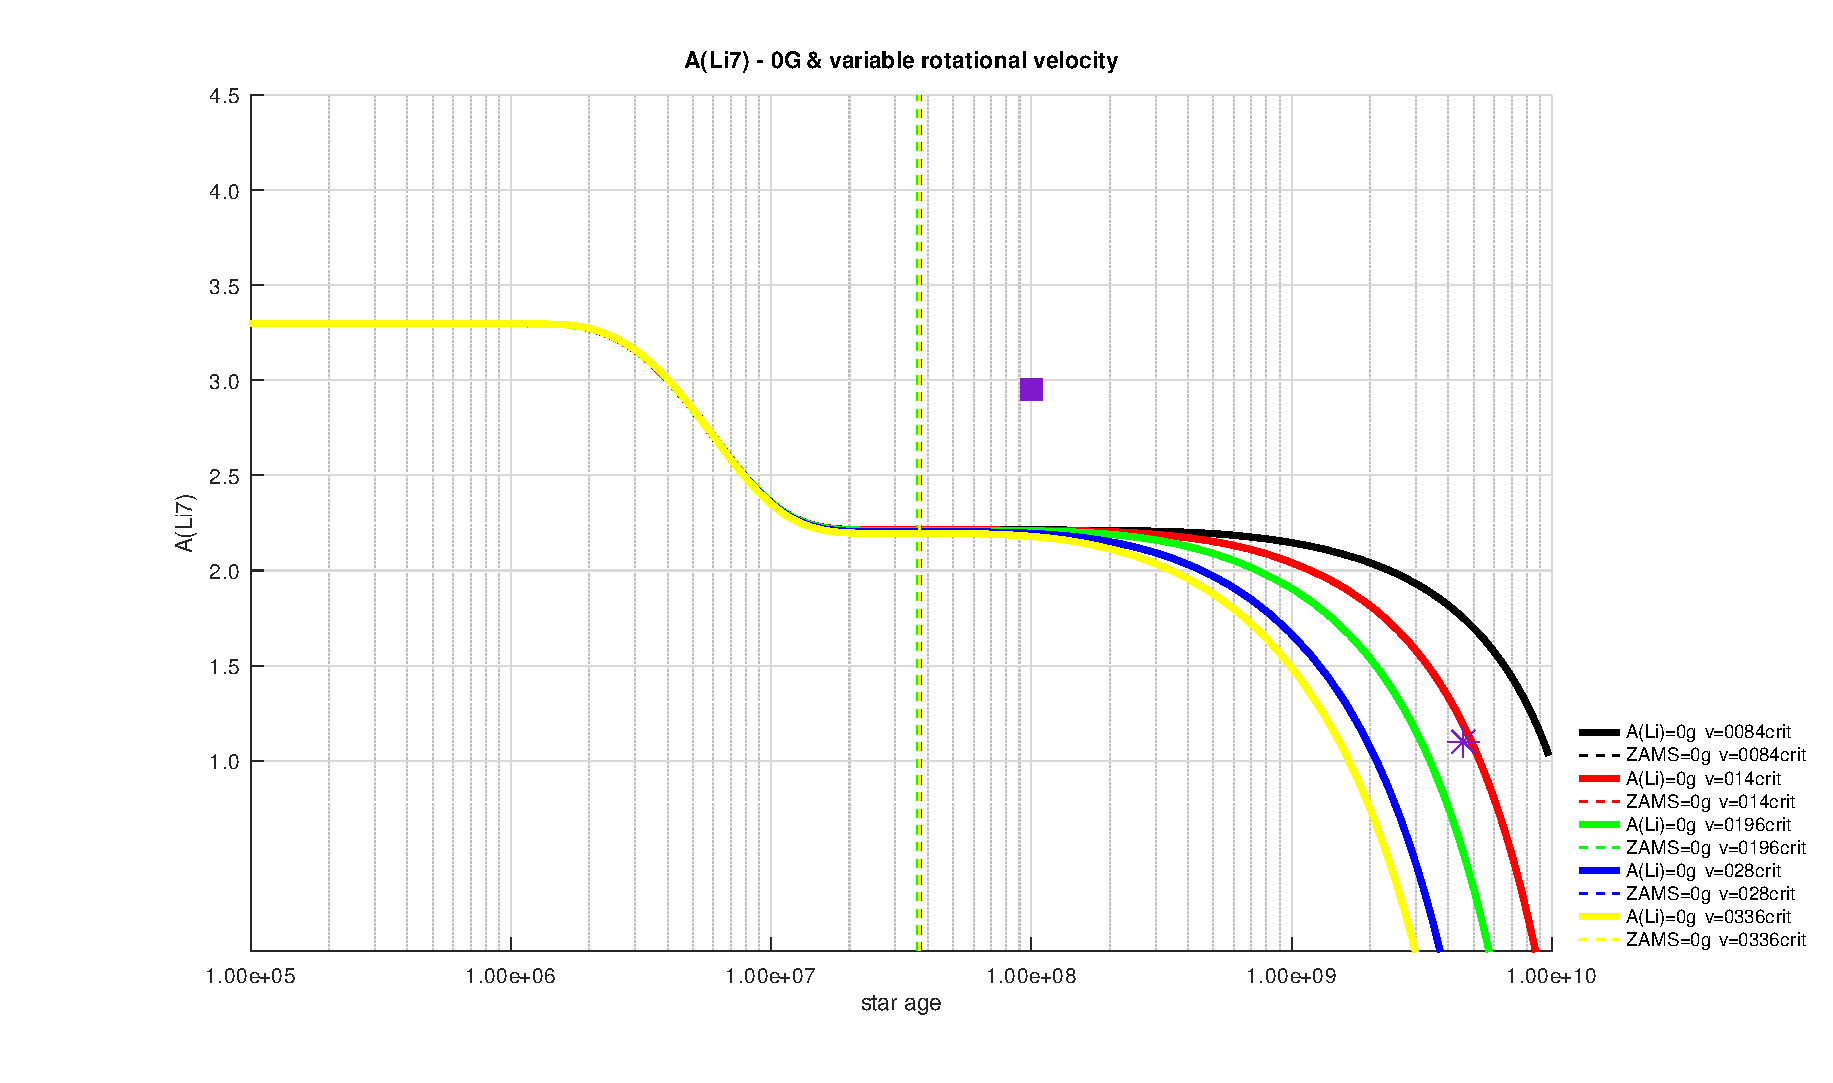
\includegraphics[trim = 35mm 15mm 20mm 15mm, clip, width=\columnwidth]{figures/li_var_vel_0_0g.eps}
    \caption{The evolution of surface \isotope[7]{Li} abundance relative to \isotope[1]{H}, as a function of time for several 1 $\msun$ models. The solid black line represents the reference model according to \citet{Choi2016}. The rest of lines are models which include PMS rotation with $\oomegac$ between 0.0084 and 0.0336, respectively. The purple star and square are surface Li abundances for the present-day Sun \citep{Asplund2009} and the average for the Pleiades cluster \citep{Sestito2005} respectively. The dashed lines make reference to the ZAMS.}
    \label{fig:li_var_vel_0g}
\end{figure}

Figure \ref{fig:li_var_vel_0g} shows the evolution of surface Li abundance relative to H as a function of time and for several $1\msun$ models initialized with different rotational velocities. The simulations take into account the effects of rotation and AML caused by stellar winds but not those of MB. The purple star and square are the surface Li abundances for the present-day Sun \citep{Asplund2009} and for the Pleiades, respectively.  \citep{Sestito2005}.\par

Additionally, notice how the Li abundance in the star surface decreases over time for all simulated models. The solid black line represents the reference model that adopts the solar-calibrated envelope overshooting parameters as documented in \citet{Choi2016}. All models burn too much Li before the ZAMS and therefore do not match with the Pleiades average surface Li abundance. Also remarkable is the fact that there are barely any differences between the different models in terms of the abundance of Li for much of the PMS. Only after one million years is Li destroyed to an accentuated degree, since the necessary temperature is not reached at BCZ before. Afterwards the different models destroy the Li in a very similar way due to two main reasons. On the one hand, the convective zones that the models develop have very similar sizes, so that the temperature at the BCZ is practically the same. On the other hand, the differential rotation between the core and the convective zone does not begin to develop until it reaches $ \approx 10^6$ years, achieving its maximum difference in the ZAMS about $ \approx 10^7$ years. It is at this moment that the combined effects of turbulence and rotational difference should increase, leading to notable differences in the evolution of A(Li) (see Figure \ref{fig:li_var_vel_0g_z1}). Later, the reference model does not deplete Li efficiently on the MS and fail (again) to match the current solar surface Li abundance. On the other hand, the other models which include rotation during the PMS with values of $\oomegac$ between 0.0084 and 0.0336 are able to burn Li in a more realistic way although only one of them (green line) is close to match the present-day Li abundance of the Sun but its rotational velocity is much higher (see Figure \ref{fig:rot_vel_0g}) than the $2\,\kms$ of the Sun \citep{Gill2012}. \par

For much of the PMS the star rotates as a solid body (see Figure \ref{fig:rot_vel_0g}) and this is because the star has a completely convective interior. It is not until the end of Hayashi track that the star begins to develop a radiative core due to the increase in temperature that occurs inside the star during the contraction process. It is in this stage of evolution of the star when a difference in angular velocity appears between the upper and lower limits of the radiative and convective zones respectively. The degree of differential rotation is directly influenced by the initial $\Omega$. As the models are initialized with a higher angular velocity, the difference in velocity between the BCZ and the star surface is accentuated in a directly proportional mode; the higher the initial velocity, the bigger the velocity gradient between the bottom and top limits of the CZ. As a consequence, the turbulence strength located at the BCZ increases so that Li can reach regions with temperatures about $\tli$ where it is finally burned and destroyed (see Figure  \ref{fig:li_var_vel_0g}). Other investigations \citep{Bouvier2018, Baraffe2017}  point to a tendency diametrically opposed to the one exposed here, i.e. the faster the rotation speed, the greater the abundance of Li on the surface of the star. \par

\begin{figure}
	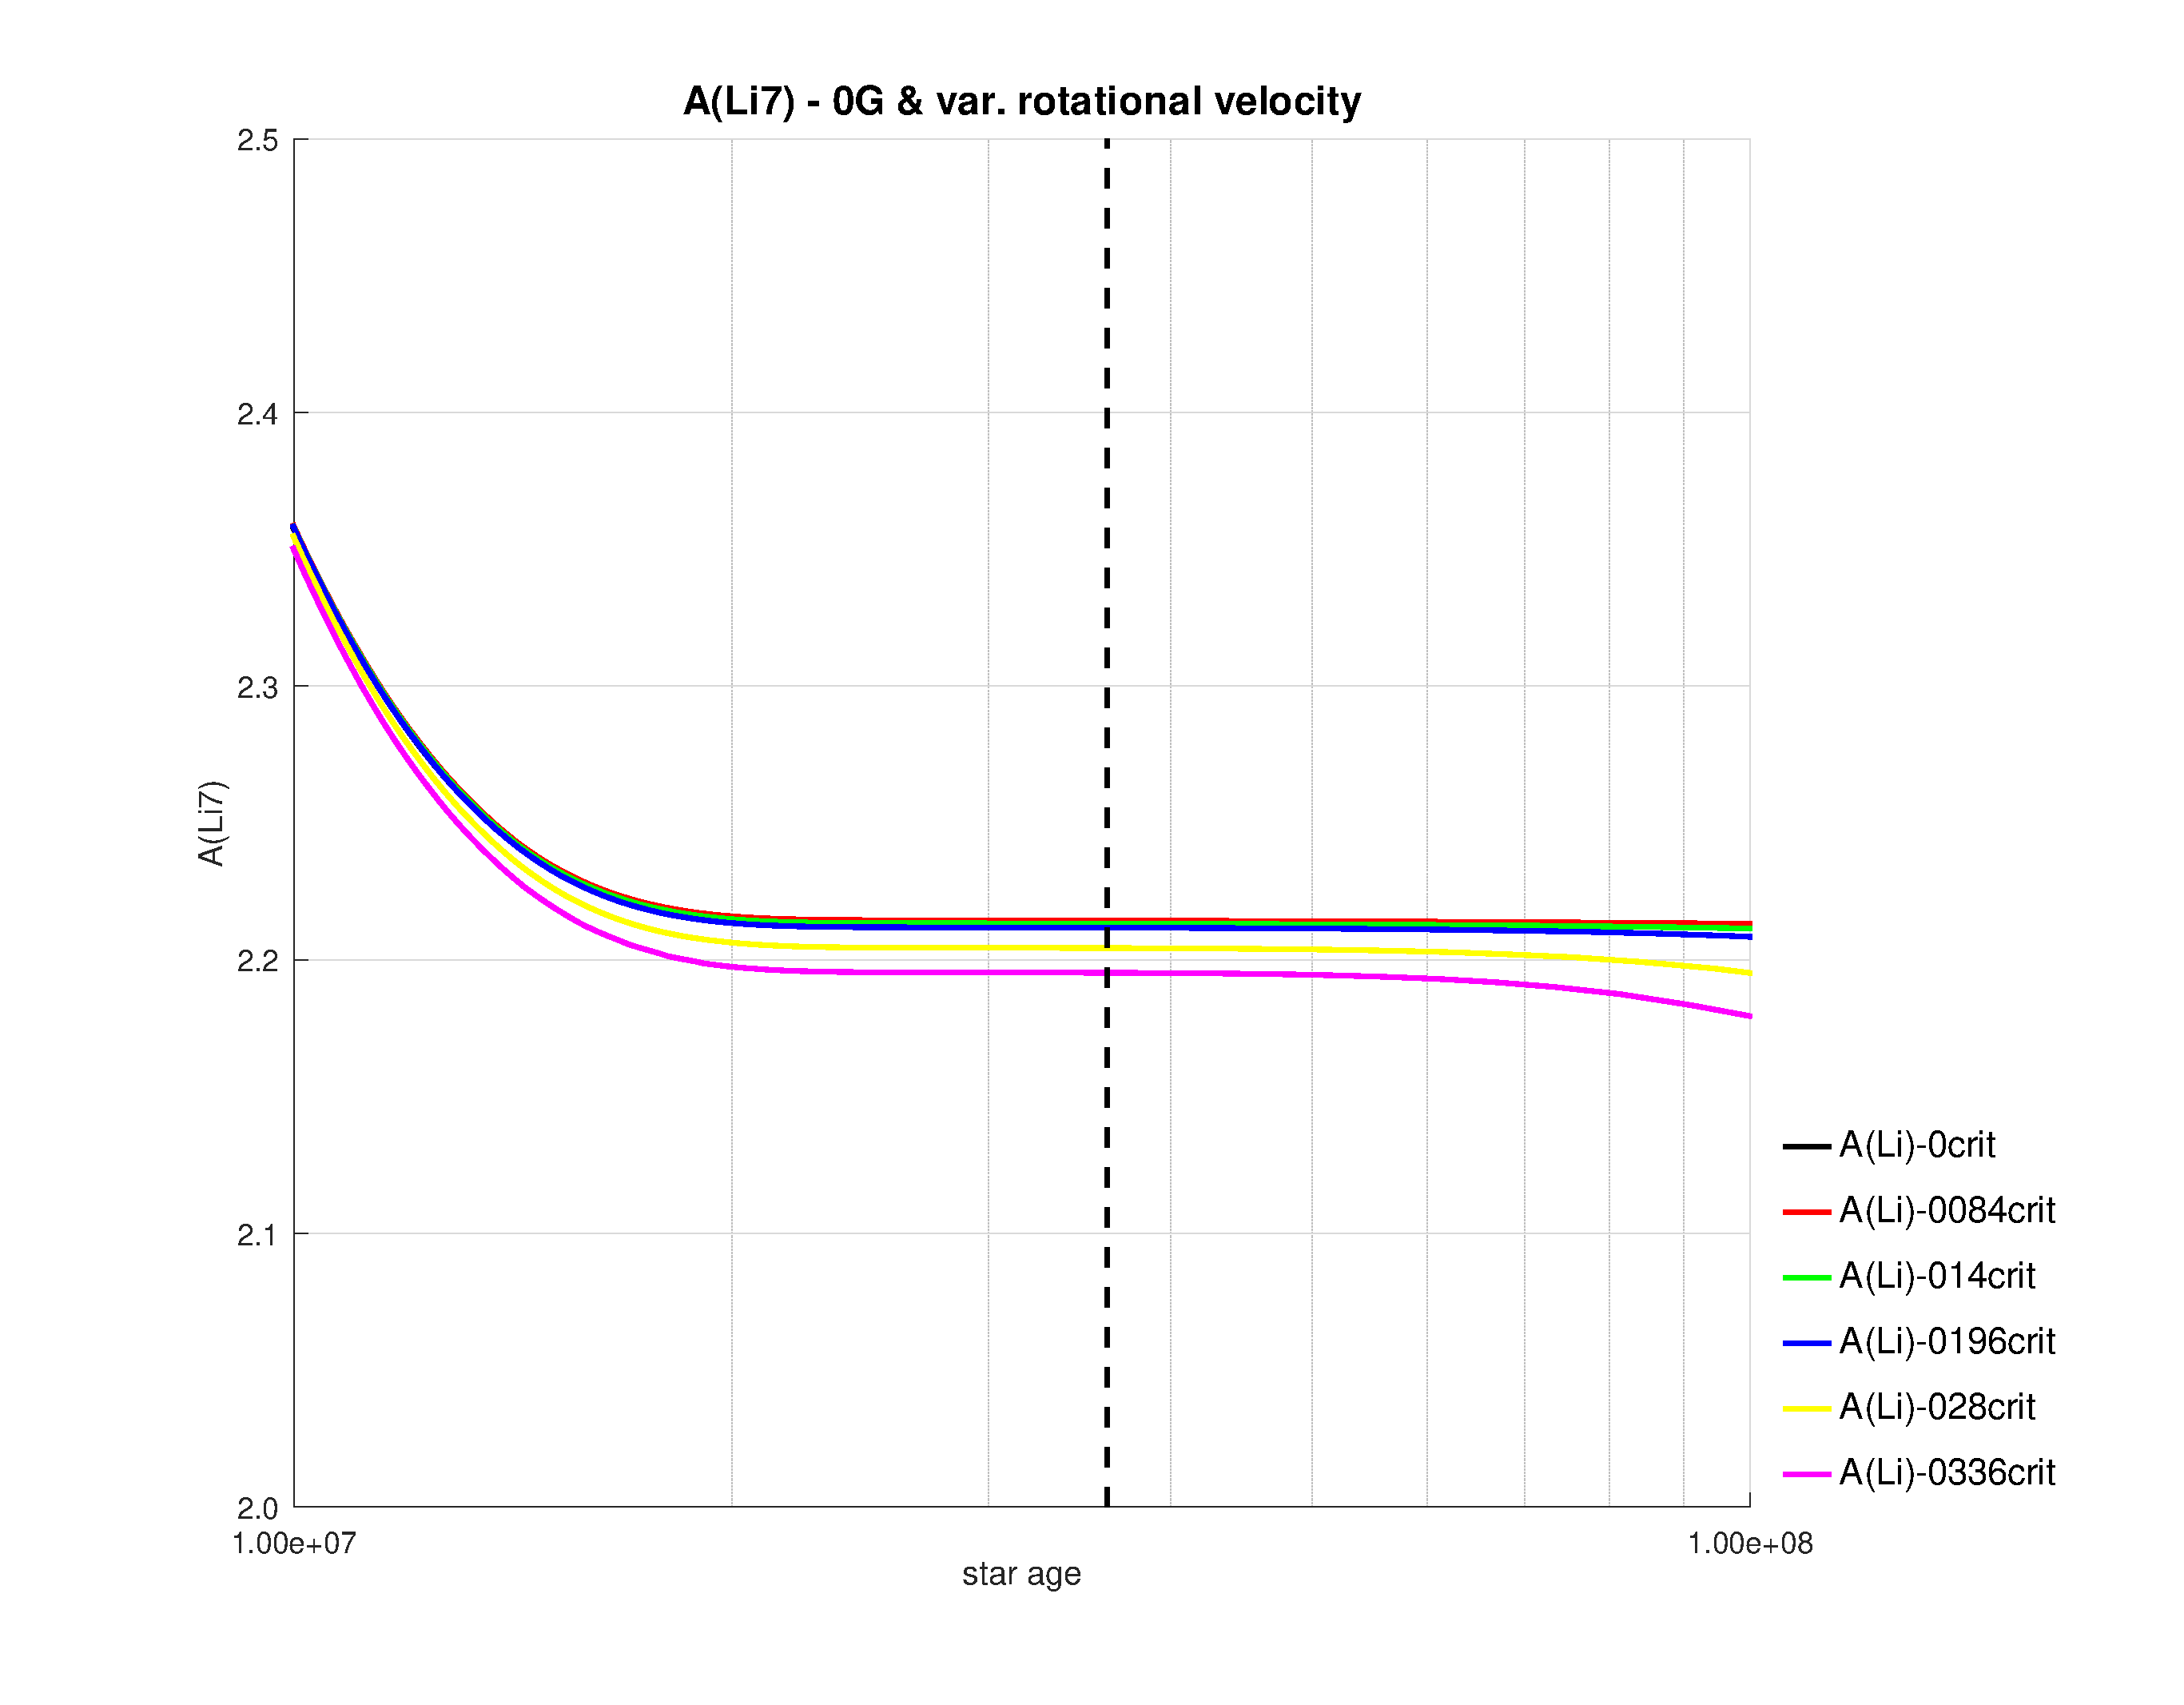
\includegraphics[trim = 35mm 15mm 20mm 15mm, clip,width=\columnwidth]{figures/li_var_vel_0_0g_z1.eps}
    \caption {Similar to Figure \ref{fig:li_var_vel_0g} but zooming in on the ZAMS. The models with a higher initial rotational velocity reach already the ZAMS with a lower amount of Li measure on the star surface.}
    \label{fig:li_var_vel_0g_z1}
\end{figure}

\begin{figure}
	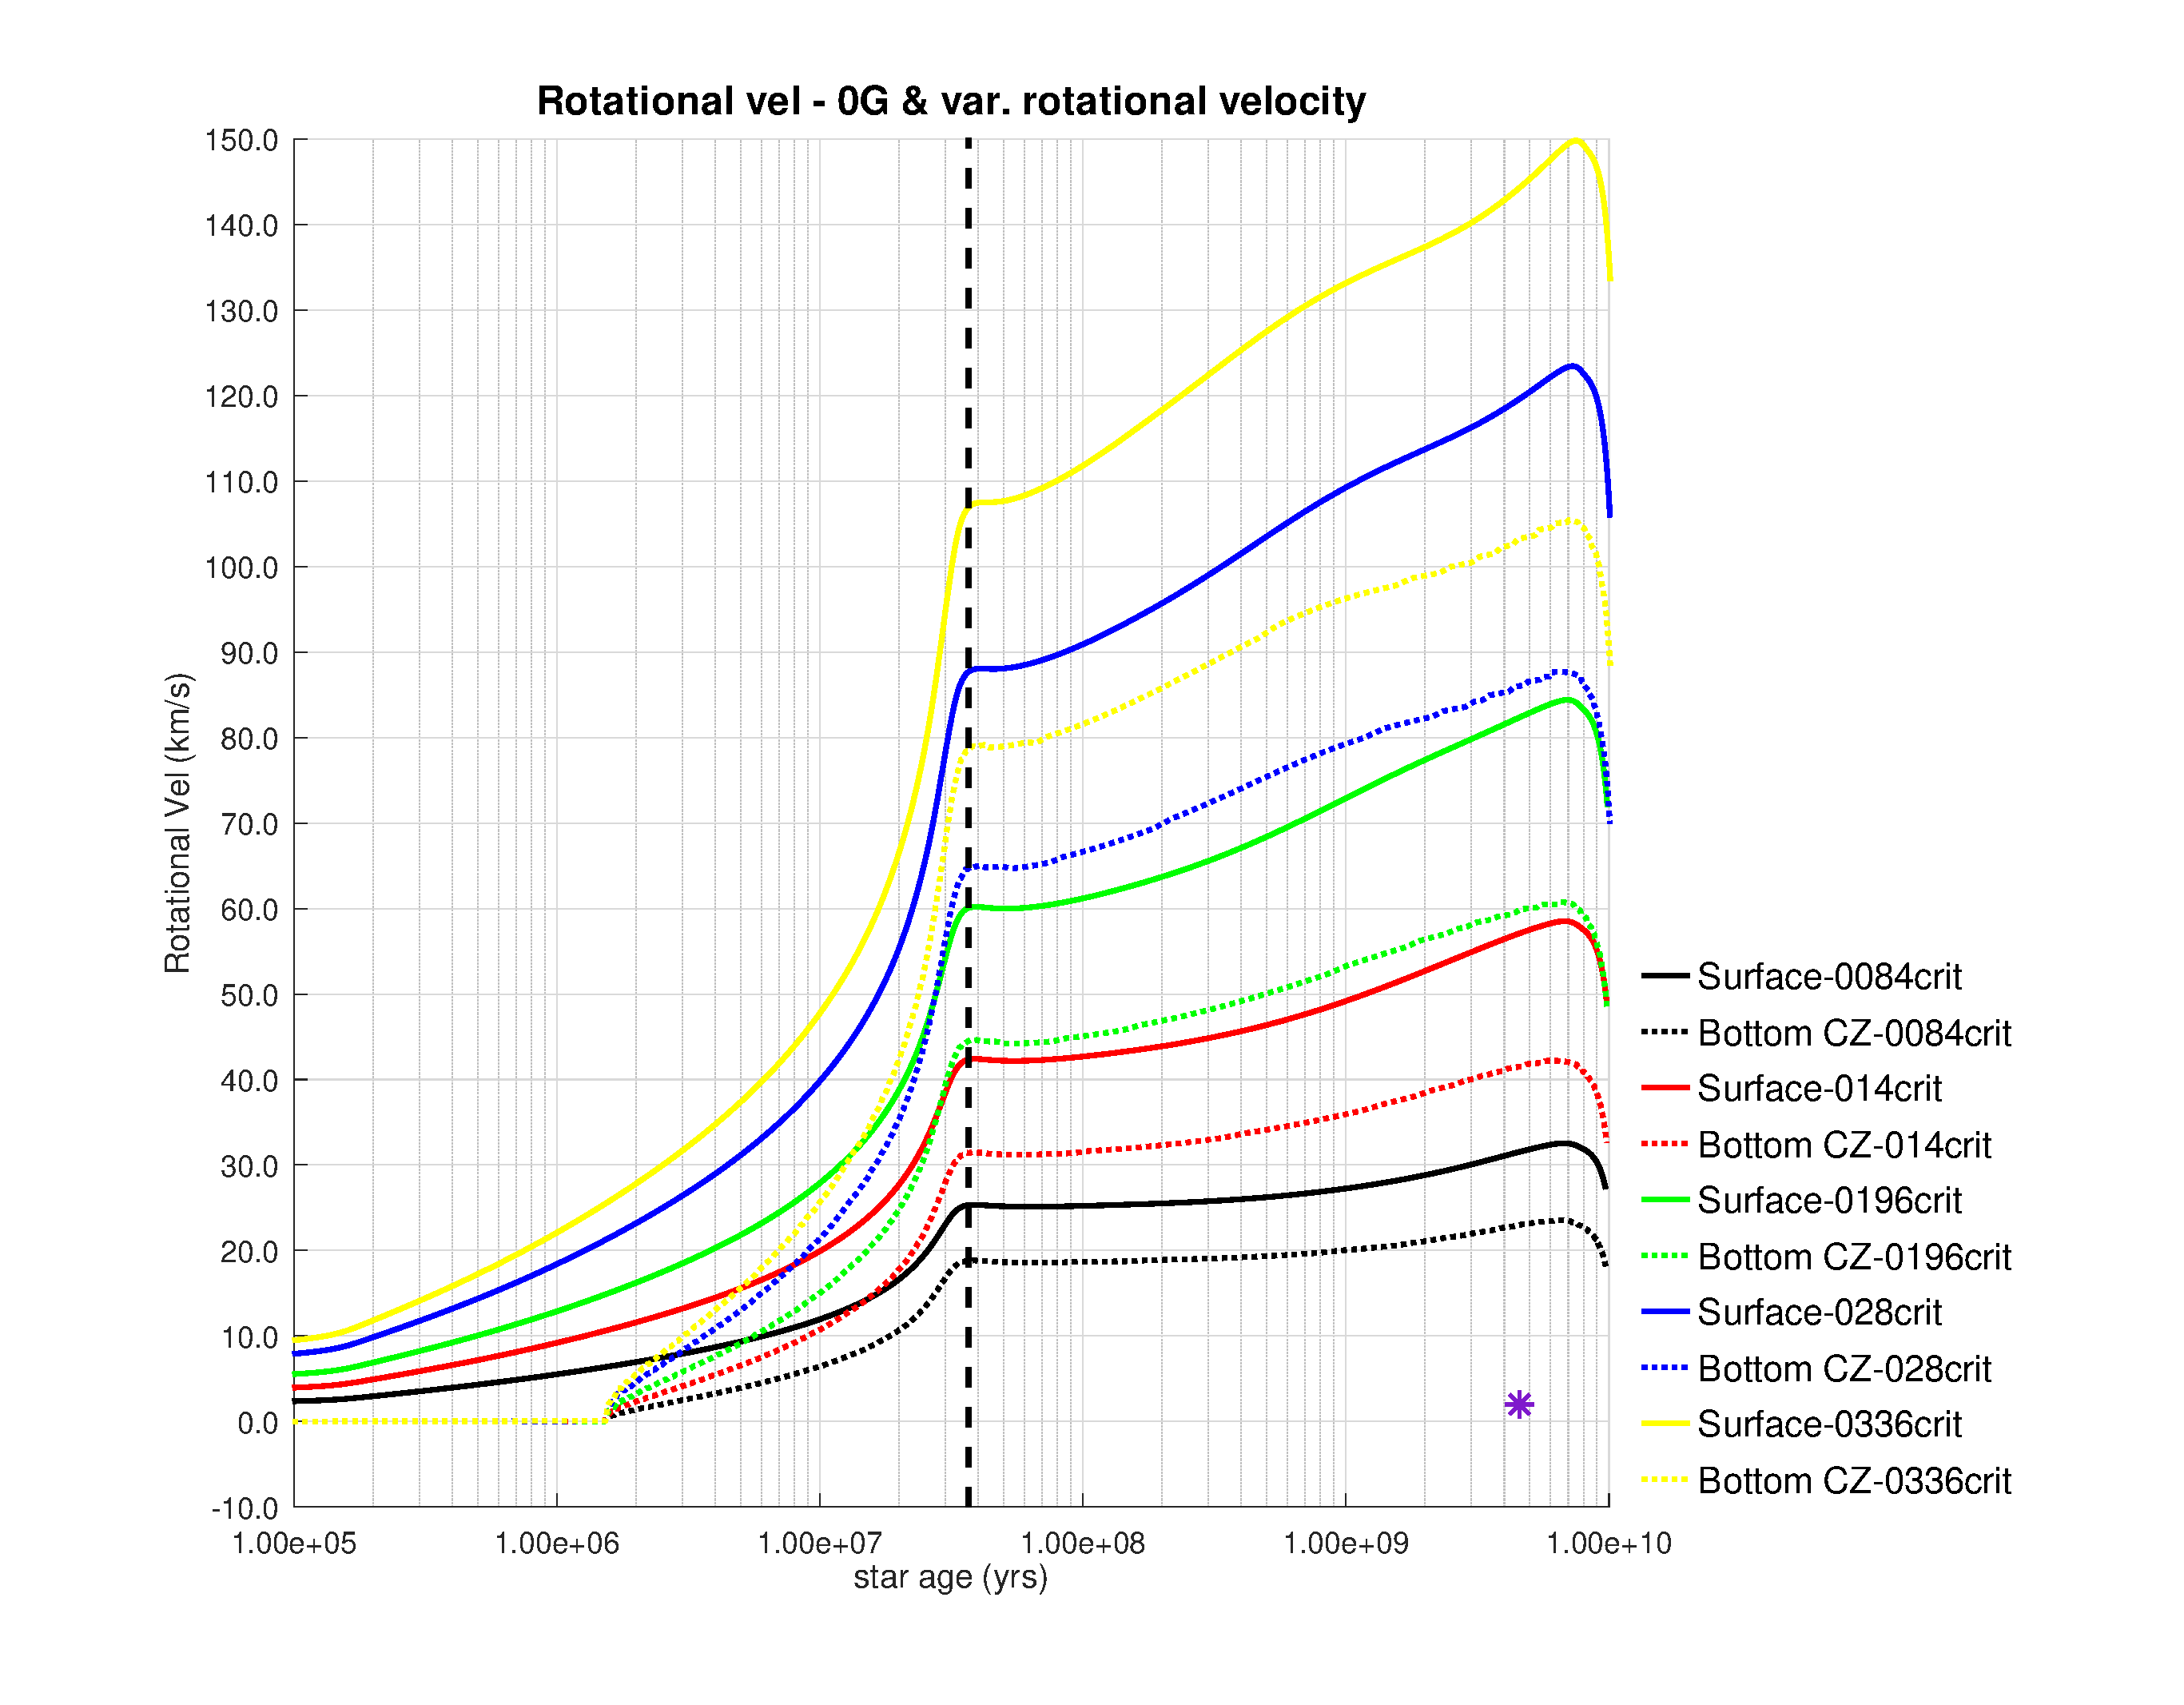
\includegraphics[trim = 30mm 15mm 20mm 15mm, clip,width=\columnwidth]{figures/rot_vel_var_vel_0_0g.eps}
    \caption{The evolution of angular velocity at surface (solid line) and at the bottom (dotted line) limit of the uppermost convective zone, as a function of time for several 1 $\msun$ models. The models includes PMS rotation with $\oomegac$ values between 0.0084 and 0.0336. The purple star is the surface angular velocity for the present-day Sun \citep{Gill2012}. The dashed vertical lines make reference to the ZAMS.}
    \label{fig:rot_vel_0g}
\end{figure}

Another well known structural effect of rotation is the decrease of the effective temperature ($\teff$) and to a less extent of stellar luminosity ($L$). Both effects can be observed graphically in the HR diagram of Figure \ref{fig:hr_var_vel_0g} which shows a zoomed-in view of evolutionary tracks from the ZAMS until the TAMS for several $1\msun$ models initialized with different rotational velocities. If we compare the non-rotating model (black solid line on the left side) with the rotating ones we can recognize that at the end of the PMS, the latter reach before the ZAMS and exhibit a lower $\teff$ than the former. These results are in line with those of previous studies \citep[see e.g. ][]{Eggenberger2012,Piau2001,Pinsonneault1989}.\par
%(see e.g. \citet{Eggenberger2012}, \citet{Piau2001}, \citet{Pinsonneault1989}).\par


\begin{figure}
	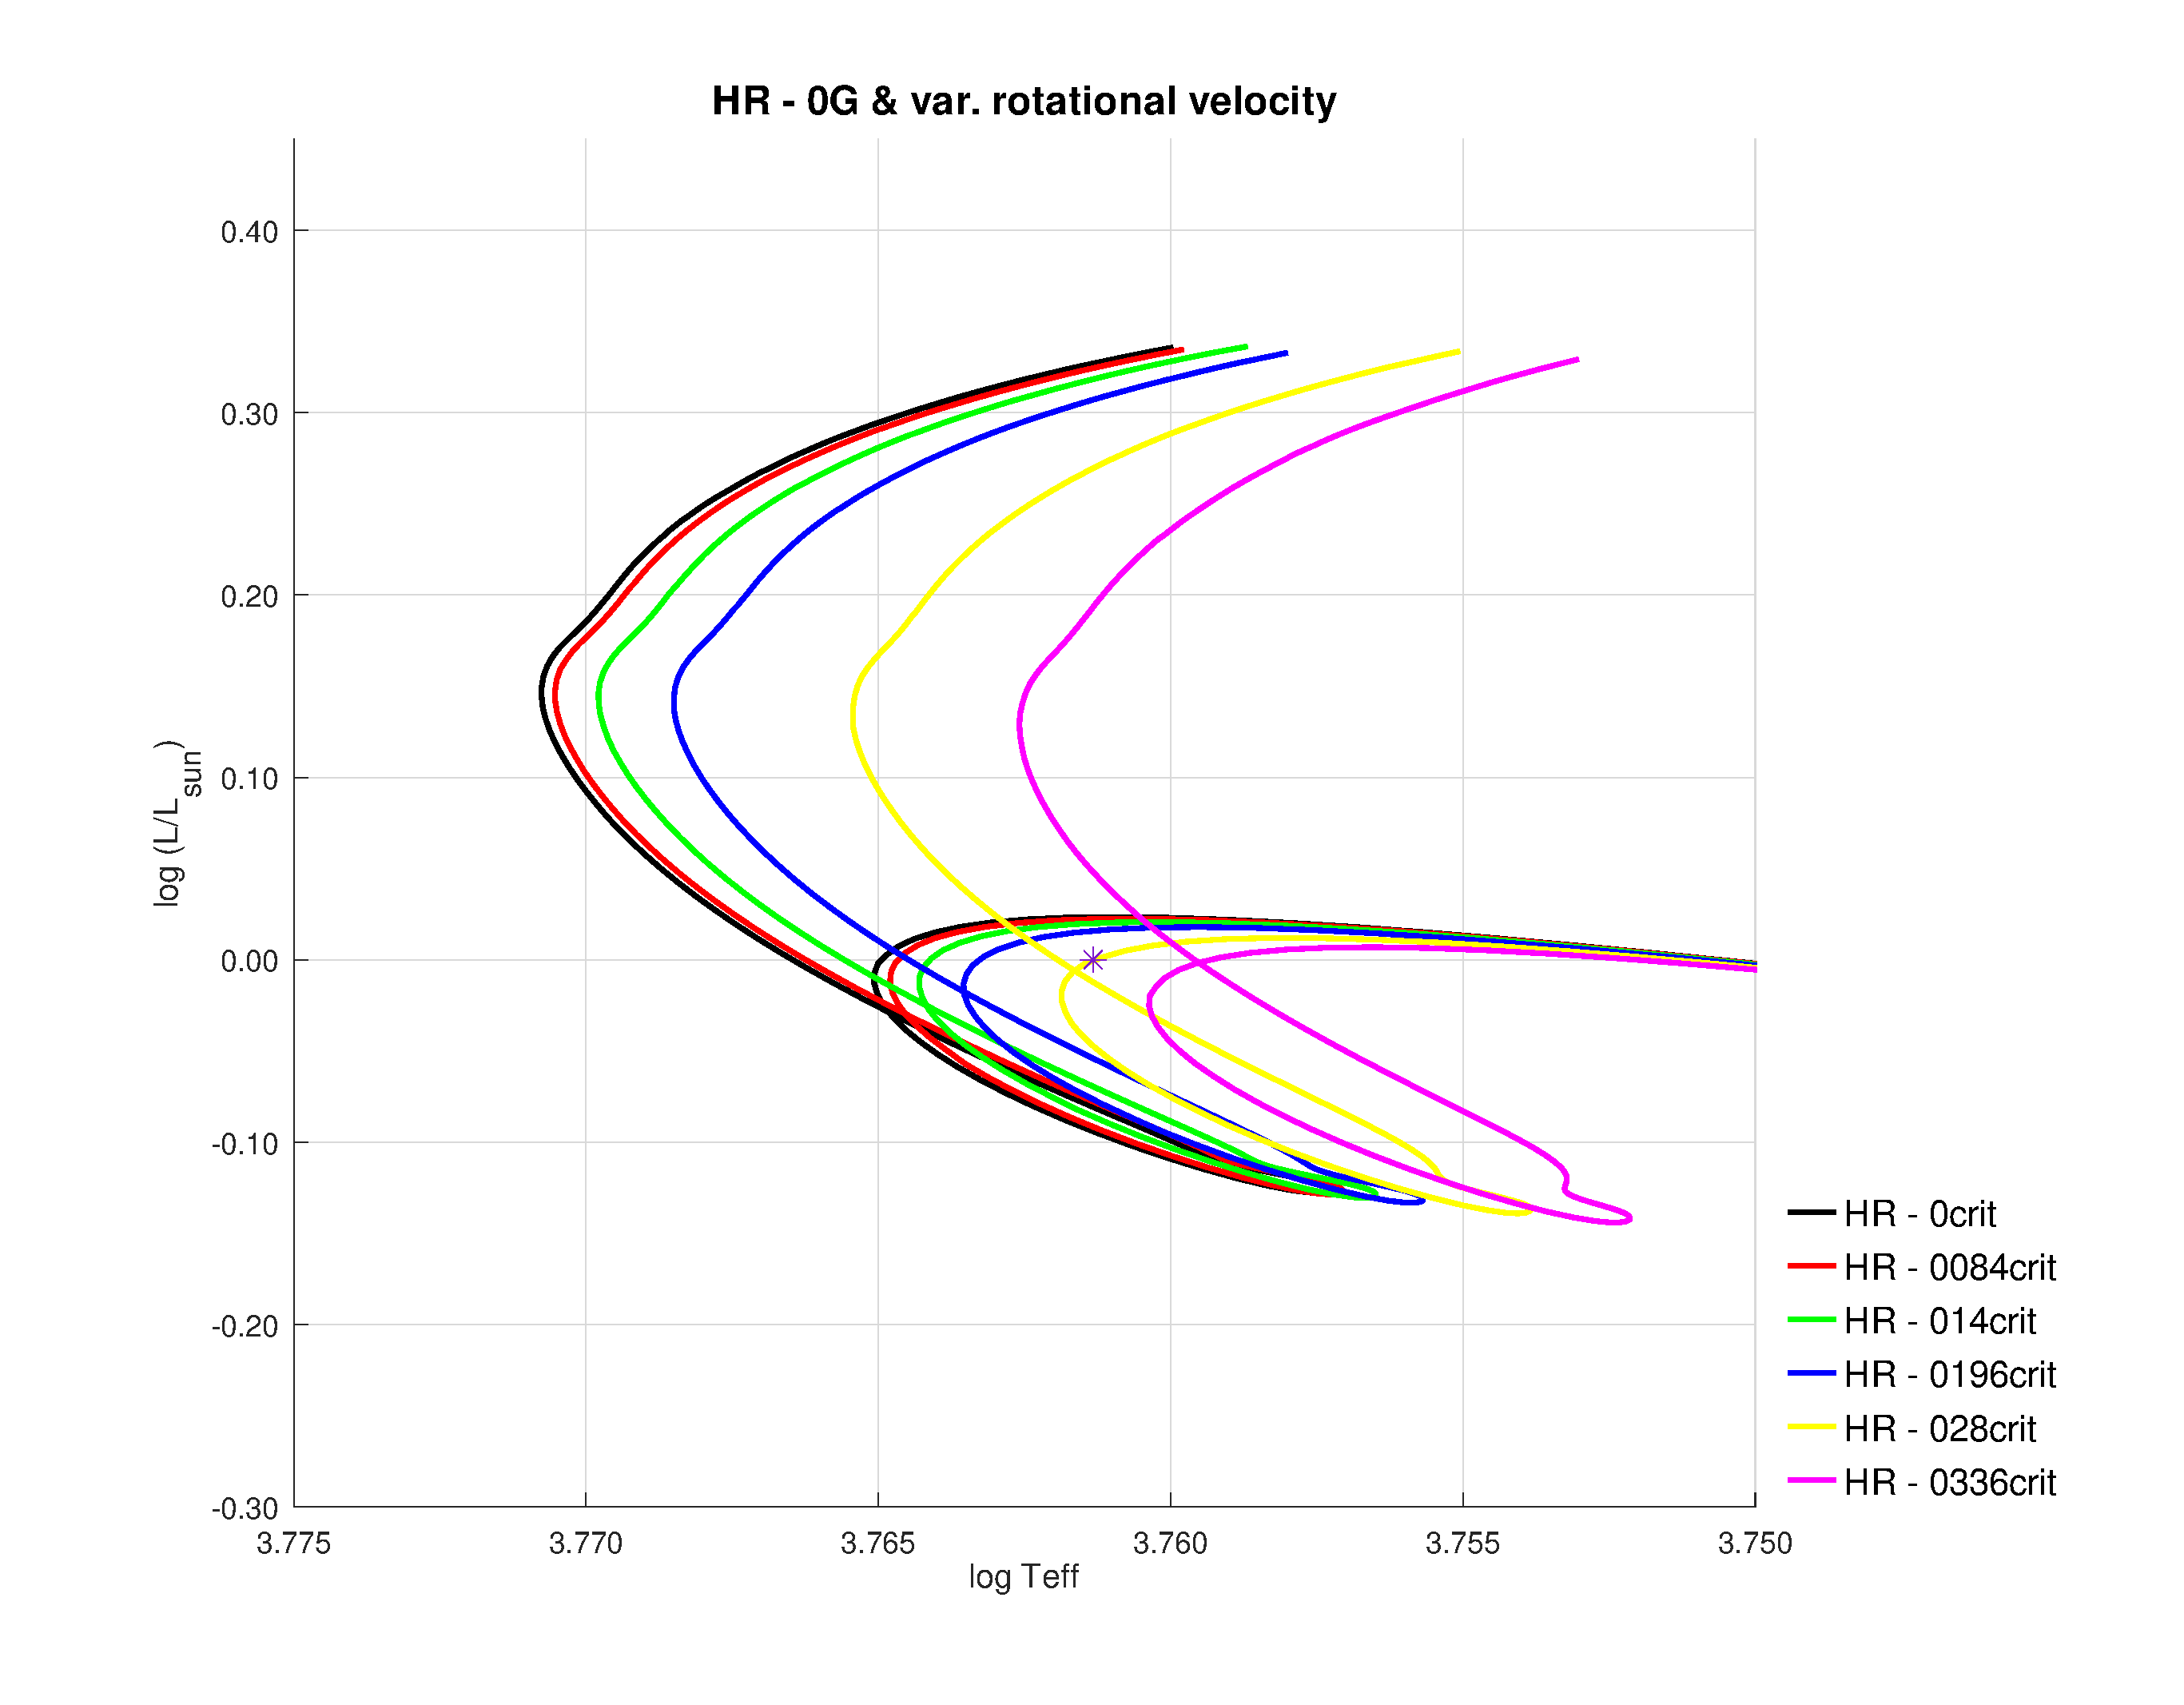
\includegraphics[trim = 30mm 15mm 20mm 15mm, clip,width=\columnwidth]{figures/hr_var_vel_0_0g_z1.eps}
    \caption{An example solar 1$\msun$ grid of stellar evolutionary track from PMS till TAMS covering a wide range of angular velocities. The rotation is activated in the models in the PMS and those models reach before the ZAMS and at a lower $\teff$ than the non-rotating one (solid black line). The luminosity is expressed in terms of $\lsun$.}
    \label{fig:hr_var_vel_0g}
\end{figure}

\subsection{Li evolution with MB}
In the rest of this document we are going to focus, unless otherwise indicated, on models that include rotation from the PMS since they are the ones that can offer a greater approximation to the observations.\par

Figure \ref{fig:li_var_vel_4_0g} shows the evolution of surface \isotope[7]{Li} abundance relative to \isotope[1]{H}, as a function of time for several 1 $\msun$ models. Those models were initialized with different rotational velocities and took into consideration both the effects of AML and the MB caused by a magnetic field of intensity 4G. If we compare it with Figure \ref{fig:li_var_vel_0g} in which the effects of MB are neglected, we notice how the profiles of Li abundance are altered during PMS and MS. In the first phase we can describe the effect as modest, somewhat expected and in line with the fact that the AML caused by MB (see Eq.~\ref{eq:j_dot}) depends directly on the mass loss rate. If we take into account that for solar-type stars the models predict a modest total mass loss rate, that value is even much lower during PMS. On the contrary, during the MS it is observed that the AML is much more significant, causing the star to rotate more slowly and as a result a smaller amount of Li to be destroyed.\par

\begin{figure}
	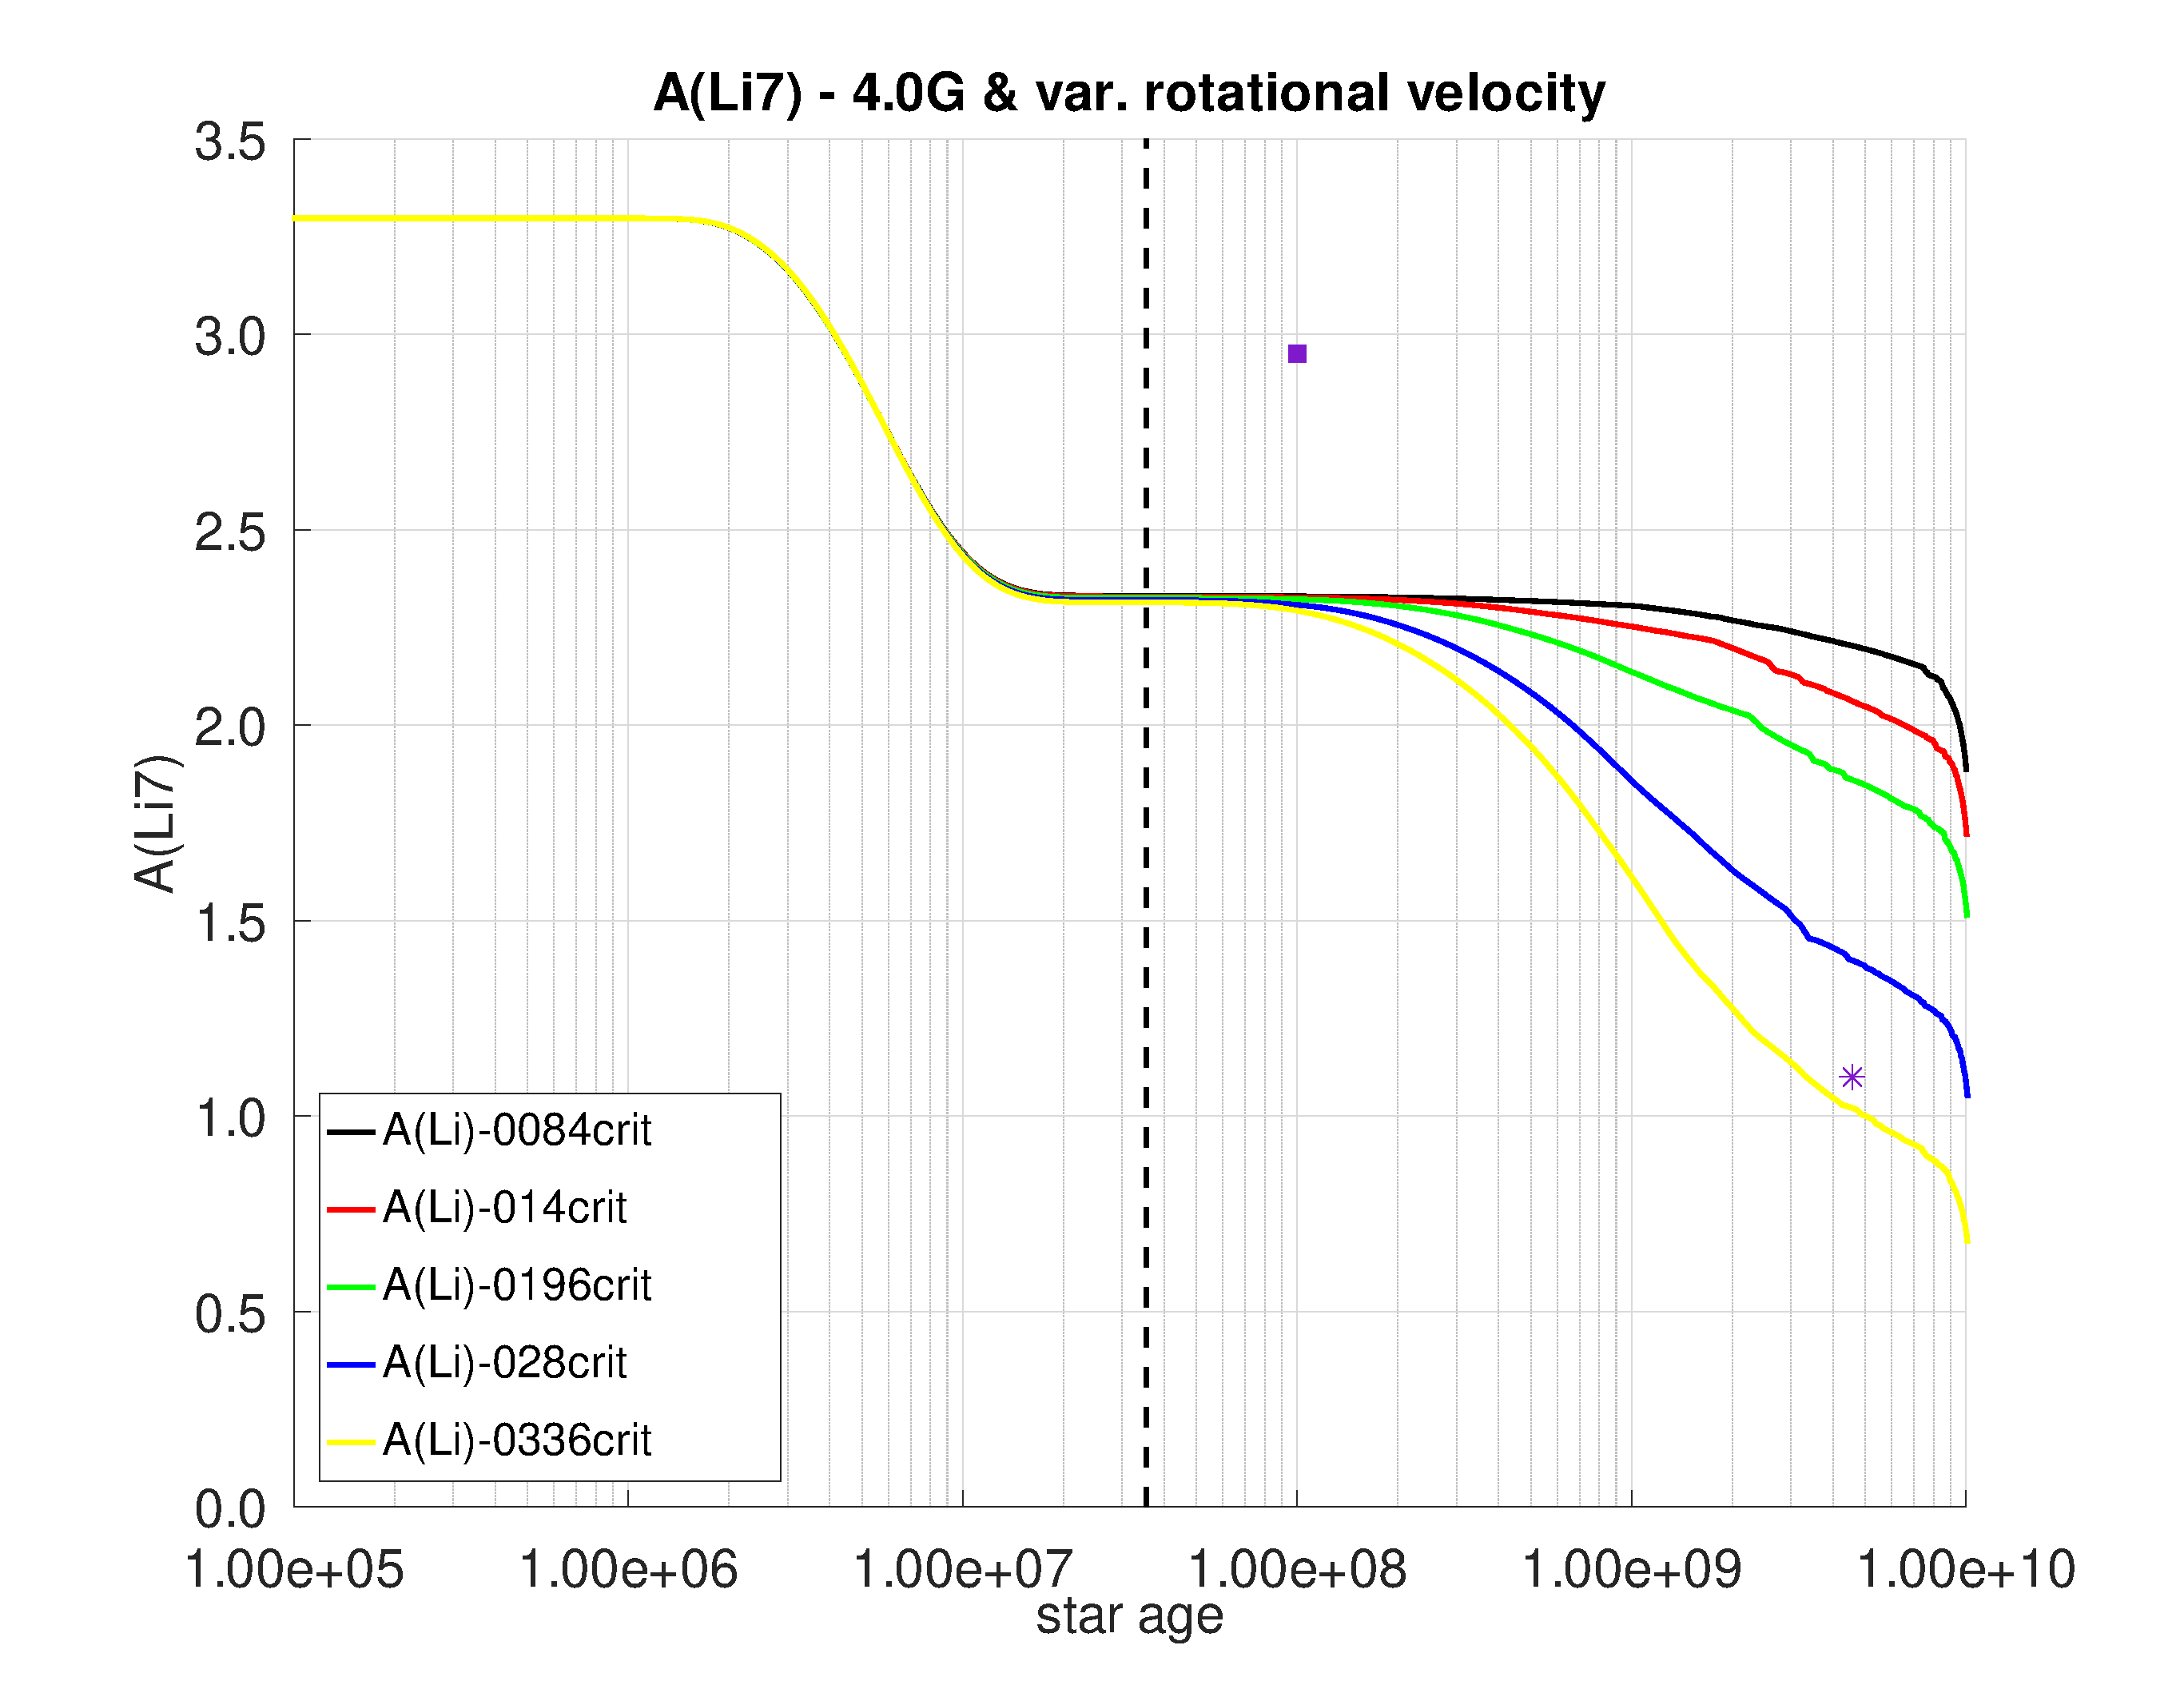
\includegraphics[trim = 35mm 15mm 20mm 15mm, clip,width=\columnwidth]{figures/li_var_vel_4_0g.eps}
    \caption{The evolution of surface \isotope[7]{Li} abundance relative to \isotope[1]{H}, as a function of time for several 1 $\msun$ models. The models include a magnetic field with an intensity of 4G and PMS rotation with $\oomegac$ between 0.0084 and 0.0336, respectively. The purple star and square are surface Li abundance for the present-day Sun \citep{Asplund2009} and the Pleiades cluster \citep{Sestito2005} respectively. The dashed lines make reference to the ZAMS.}
    \label{fig:li_var_vel_4_0g}
\end{figure}

The effect of the MB routine can be seen even more clearly in Figures~\ref{fig:rot_vel_4g}, \ref{fig:rot_vel_4g_z1} \& Appendixes \footnote{The appendices comprise a series of grids as a function of time and for several 1 $\msun$ models in which on the one hand, the evolution of surface \isotope[7]{Li} abundance relative to \isotope[1]{H} for both variable magnetic field intensities and angular velocities and on the other hand, the evolution of surface rotational velocity are shown.}. In those figures we represent the rotation profiles for the surface of the stars and for the bottom of the convective envelope for a number of 1 $\msun$ models initialized with different rotational velocities and considering the influence of MB. Similarly to the evolution profiles of the Li on the surface commented in the previous paragraph, the effect of the routine is visible once the ZAMS is reached. If we compare the evolution of the curves presented here with those of Figure \ref{fig:rot_vel_0g} we see how the star, instead of continuing to increase its $\Omega$, begins to slow down after having reached its maximum in the passage through the ZAMS. It is also at this stage when the angular velocities at the surface of the star and at the BCZ reach their maximum difference. On the other hand, the effect of magnetic braking causes the angular velocities between both zones of the star to decrease until, for an age close to that of the Sun (see Figure \ref{fig:rot_vel_4g_z1}), the star practically rotates like a rigid solid. These results are also consistent with those obtained by \citet{Eggenberger2010} as far as the effect of the magnetic field, in particular its influence on the loss of angular momentum, has on the rotational velocity of the star. In our models we have also chosen to include the rotation effects offered by MESA but not those of Spruit-Tayler (ST) dynamo on the diffusion of elements. The reason is that the implementation of MESA that makes of the ST dynamo is to simulate internal magnetic fields and not for surface magnetic fields \citep{Paxton2013}.

In a similar way we also observe that the models with lower angular velocity generally end up exhibiting higher values in the abundance of Li on the surface (see Figures~ \ref{fig:li_var_vel_4_0g}, \ref{fig:grid_li_var_vel} \& \ref{fig:grid_li_var_g}). In none of those cases we do obtain values of Li on the surface higher than those shown by the model without rotation.\par

\begin{figure}
	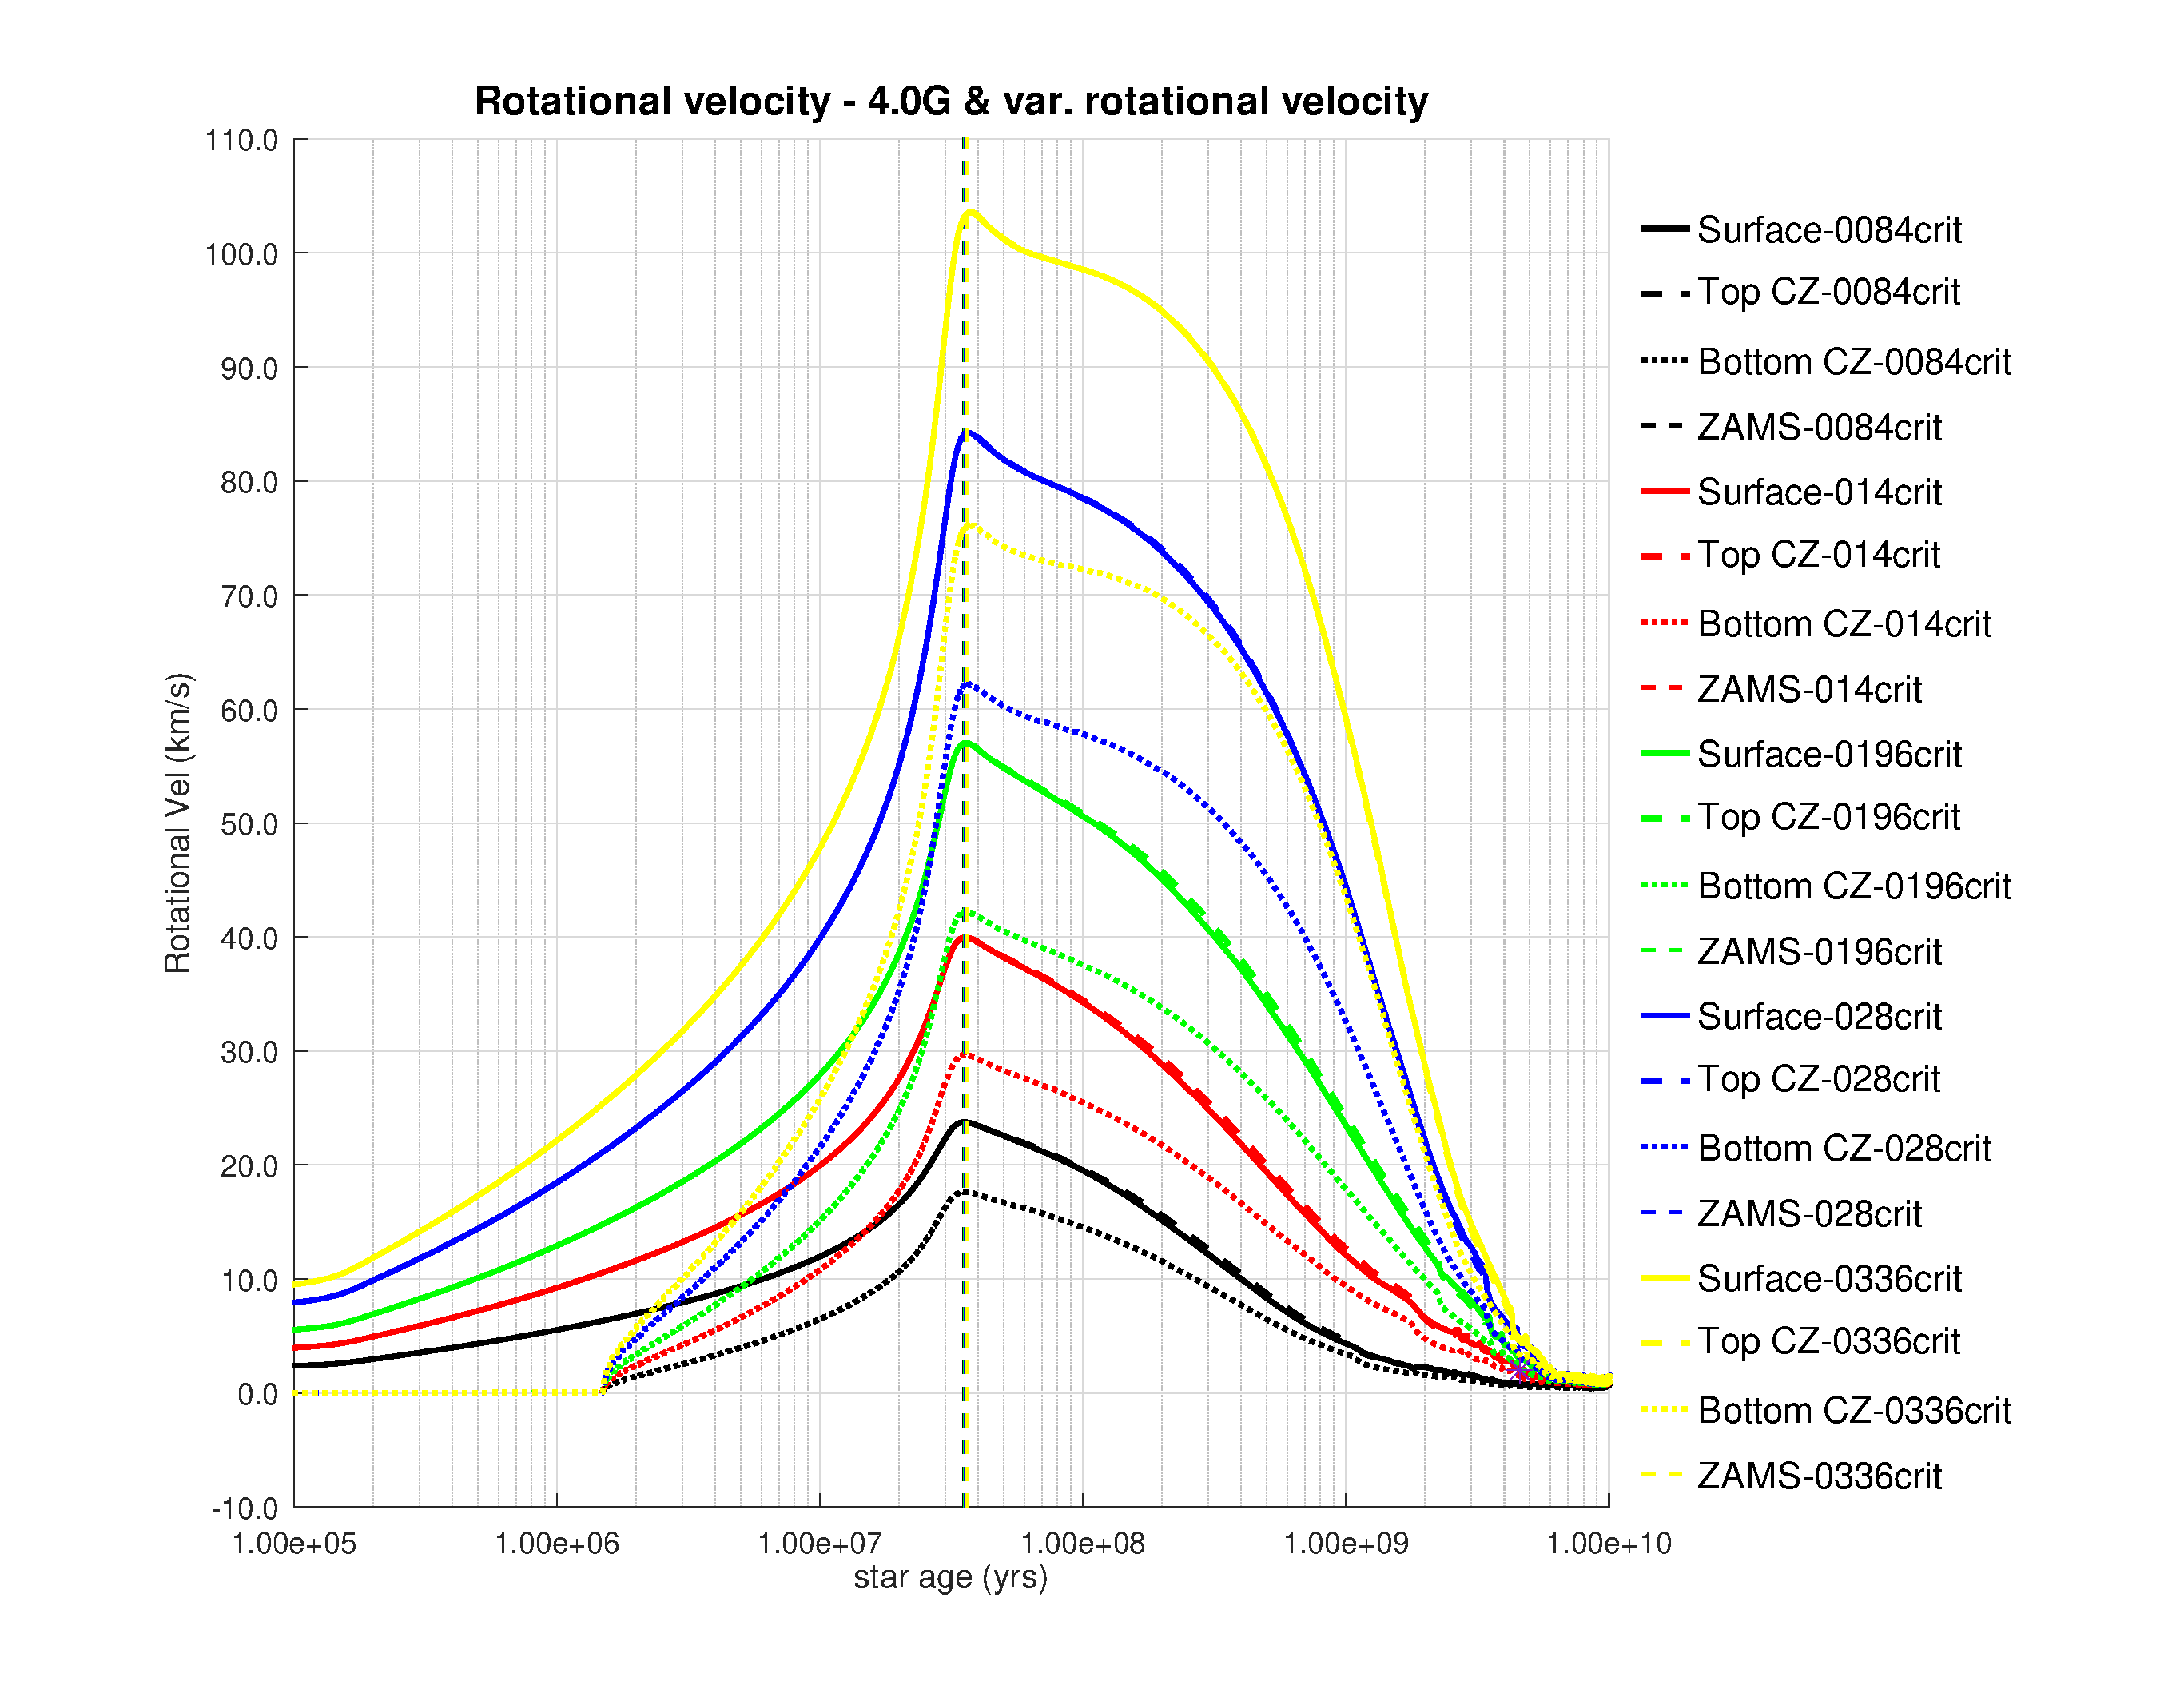
\includegraphics[trim = 30mm 15mm 20mm 15mm, clip,width=\columnwidth]{figures/rot_vel_var_vel_4_0g.eps}
    \caption{The evolution of surface rotational velocity, as a function of time for several 1 $\msun$ models. The models include a magnetic field with an intensity of 4\,G, PMS rotation with $\oomegac$ between 0.0084 and 0.0336, respectively and MB. The purple star is the surface angular velocity for the present-day Sun \citep{Gill2012}. The dashed lines make reference to the ZAMS.}
    \label{fig:rot_vel_4g}
\end{figure}

\begin{figure}
	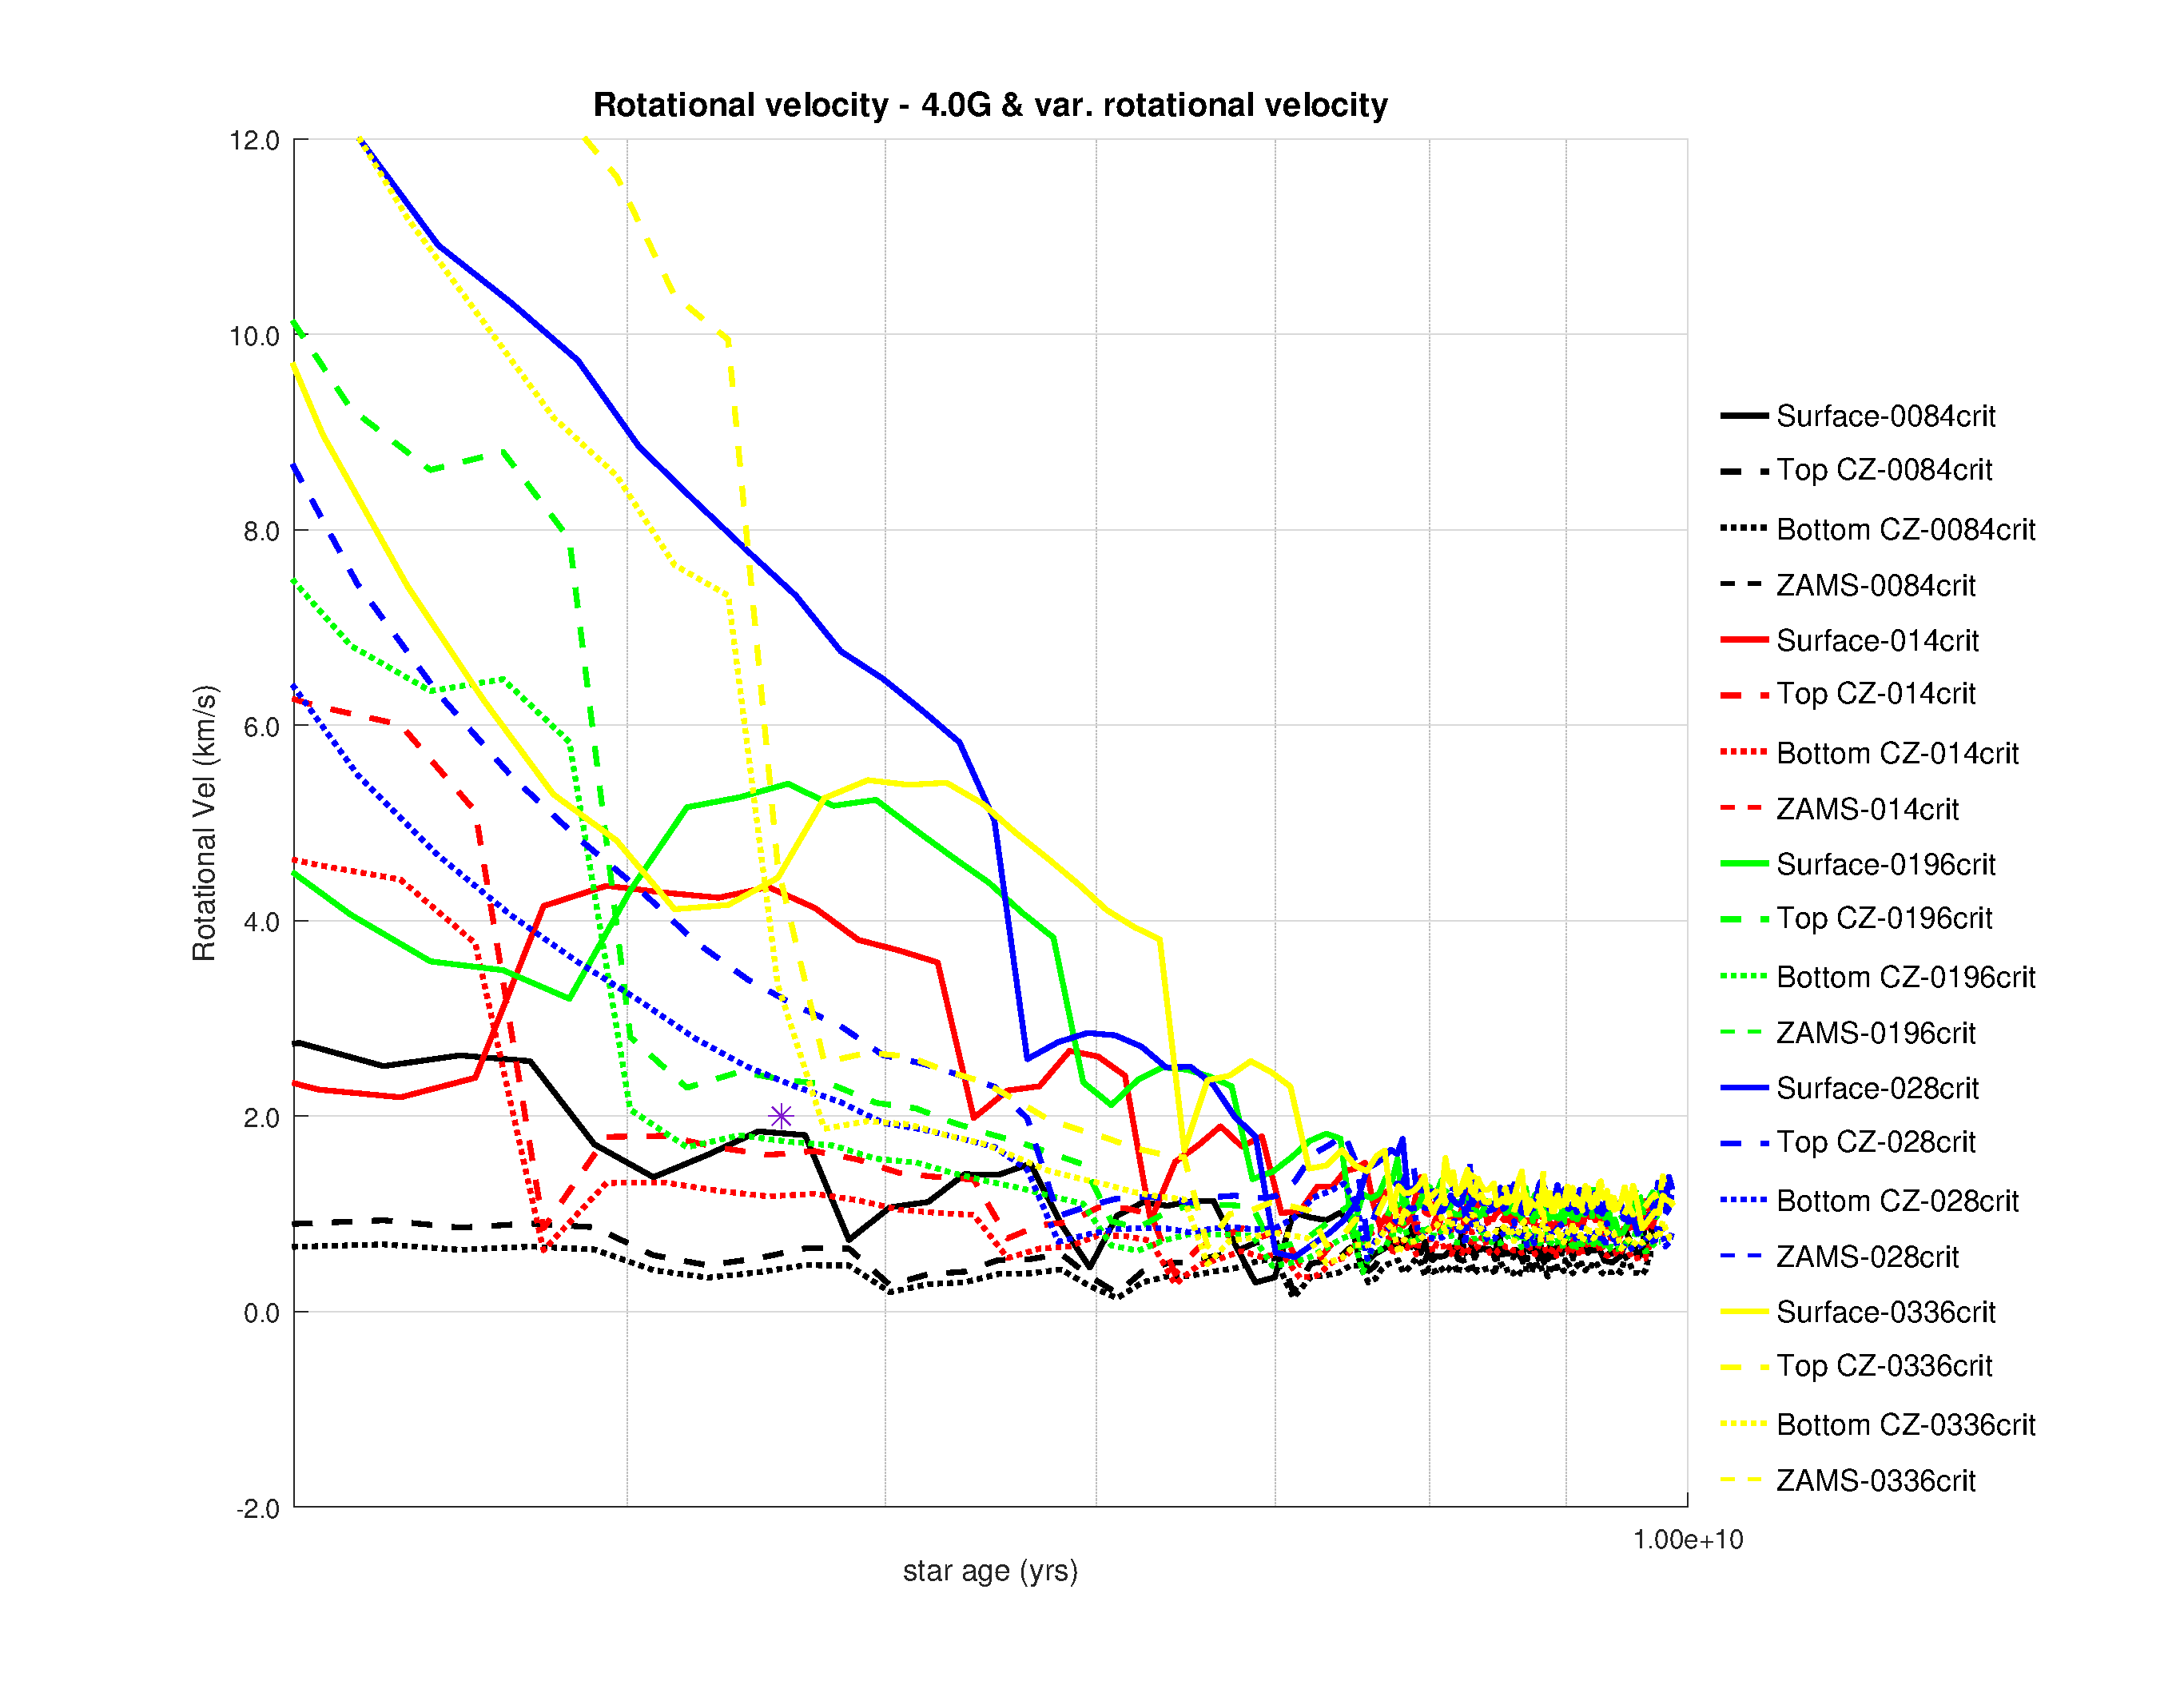
\includegraphics[trim = 30mm 15mm 20mm 15mm, clip,width=\columnwidth]{figures/rot_vel_var_vel_4_0g_z1.eps}
    \caption{Similar to Figure \ref{fig:rot_vel_4g} but now showing in detail the surface rotational velocity as the star approaches TAMS.}
    \label{fig:rot_vel_4g_z1}
\end{figure}

The MB also leaves its mark on the HR diagram by significantly affecting the $\teff$ of the star. To visualize this effect we will take as reference Figure \ref{hr_vc_0336_var_g_z1} in which all models were started with the same value $\oomegac=0.0336$ but the intensity of the simulated magnetic field was different. In particular, let us pay attention to the evolutionary trace in which a magnetic field was not simulated (black solid line) and to the rest of the evolutionary traces in which it was. We have that the group of simulations with presence of a magnetic field produces hotter stars due to the MB influence. The lower speed with which the star rotates due to the MB effect causes the increase of the $\teff$, being this difference of practically $95\,\Kelvin$ between the simulated models with $0.0\,\Gauss$ and $5.0\,\Gauss$ respectively for $log(\llsun)=0$.

\begin{figure}
	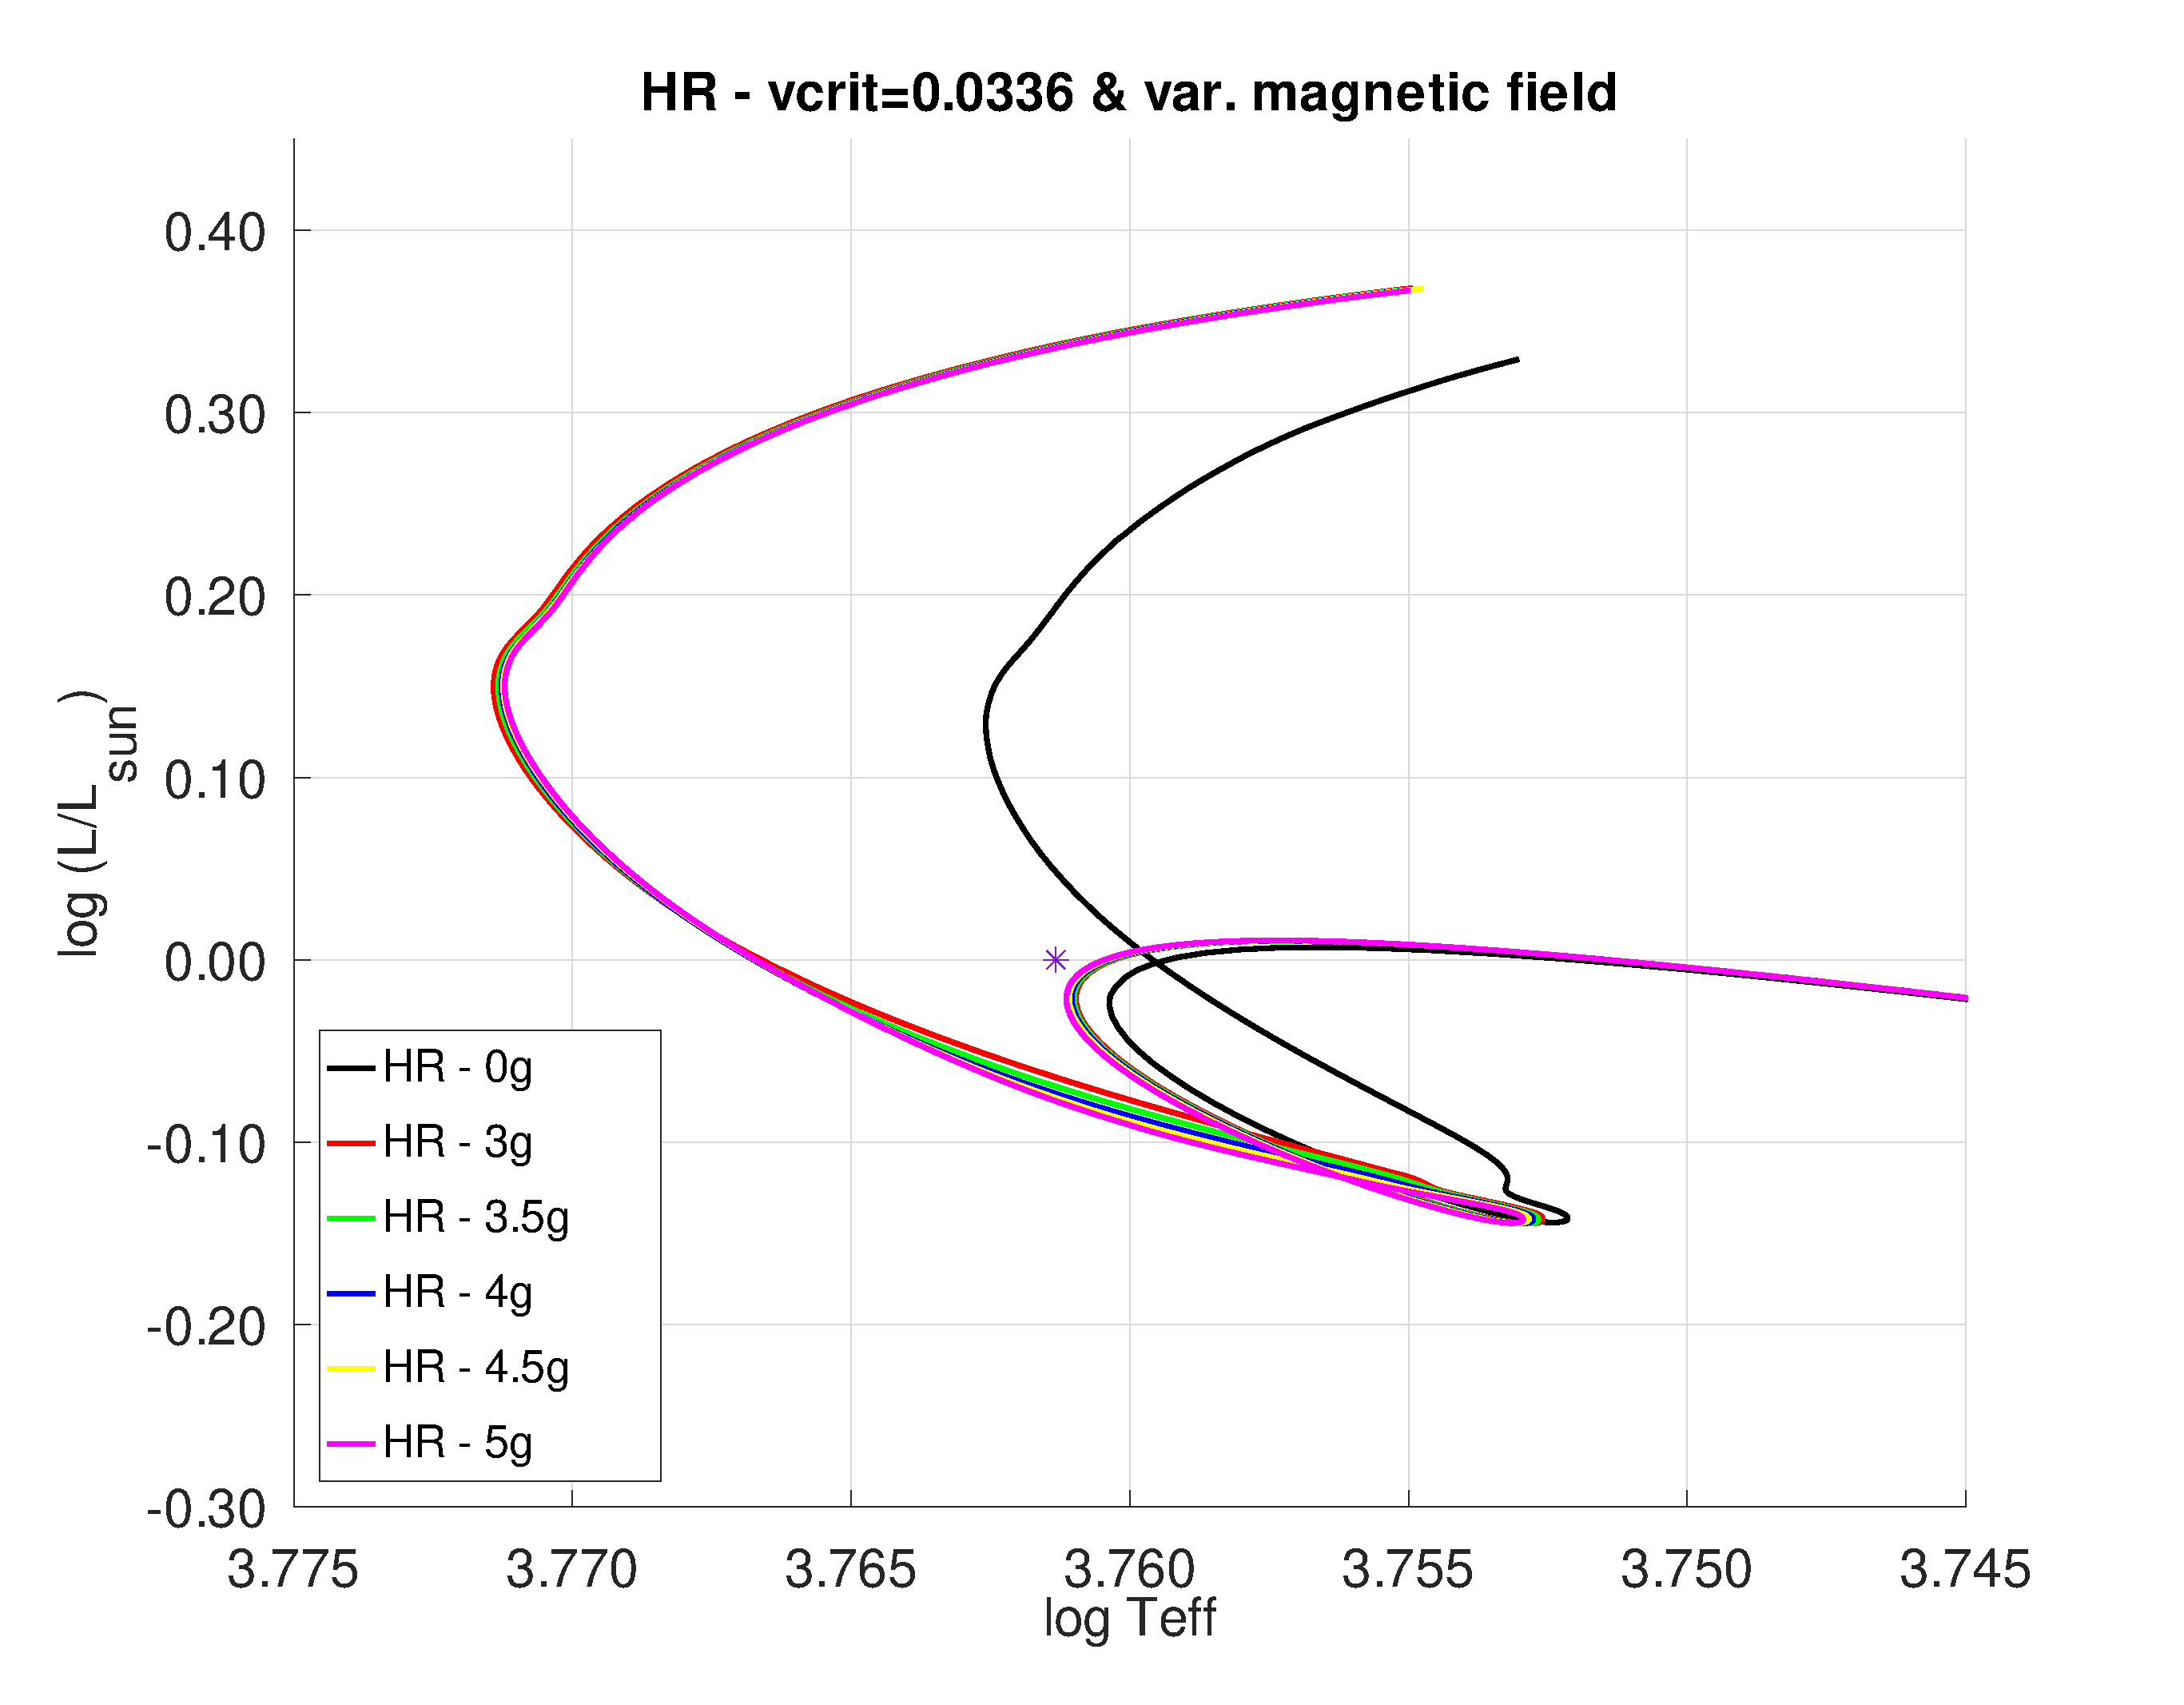
\includegraphics[trim = 30mm 15mm 15mm 15mm, clip,width=\columnwidth]{figures/hr_vc_0336_var_g_z1.eps}
    \caption{Similar to Figure \ref{fig:hr_var_vel_0g} but now showing in detail the effects of magnetic braking on the evolutionary tracks for different magnetic field strengths and $\oomegac=0.0336$. The presence of a magnetic field produces hotter stars due to the influence of the magnetic braking on the rotational velocity of the star.}
    \label{hr_vc_0336_var_g_z1}
\end{figure}



As described in section \ref{sec_mesh}, the MB routine distributes the total amount of AML calculated according to Eq.~\ref{eq:k_jdot} among the different layers that compose the CZ. In Figure \ref{fig:cz_vc_028_var_b} we can observe the evolution of the most external CZ normalized with respect to the radius of the star for several 1 $\msun$ models. The models were all initialized with $\oomegac=0.0336$ and magnetic field strengths varying between $0.0\,\Gauss$ and $5.0\,\Gauss$. In accordance with the established models of stellar evolution, in a solar-type star the CZ covers practically all of it for a large part of the PMS. As it approaches the ZAMS, the CZ is decreasing as a consequence of the appearance of a radiative core and maintains an approximately constant radius until the final stage of the MS. In this point it increases significantly as a response to the generalized expansion of the star's radius. Regarding the effect of MB on the size of the CZ, we observe that as the intensity of the magnetic field increases, the size of the CZ decreases (see Figure \ref{fig:cz_vc_028_var_b}). The radiative core pushes outward to include a rapidly increasing fraction of the stellar mass, making that the temperature at the CZ base drops below $\tli$. This effect is most evident during MS (see Figure \ref{fig:cz_vc_028_var_b_z1}). The decrease in the size of the CZ is in line with the fact that less Li is destroyed by causing less star material to reach areas with temperatures above $\tli$.\par

\begin{figure}
	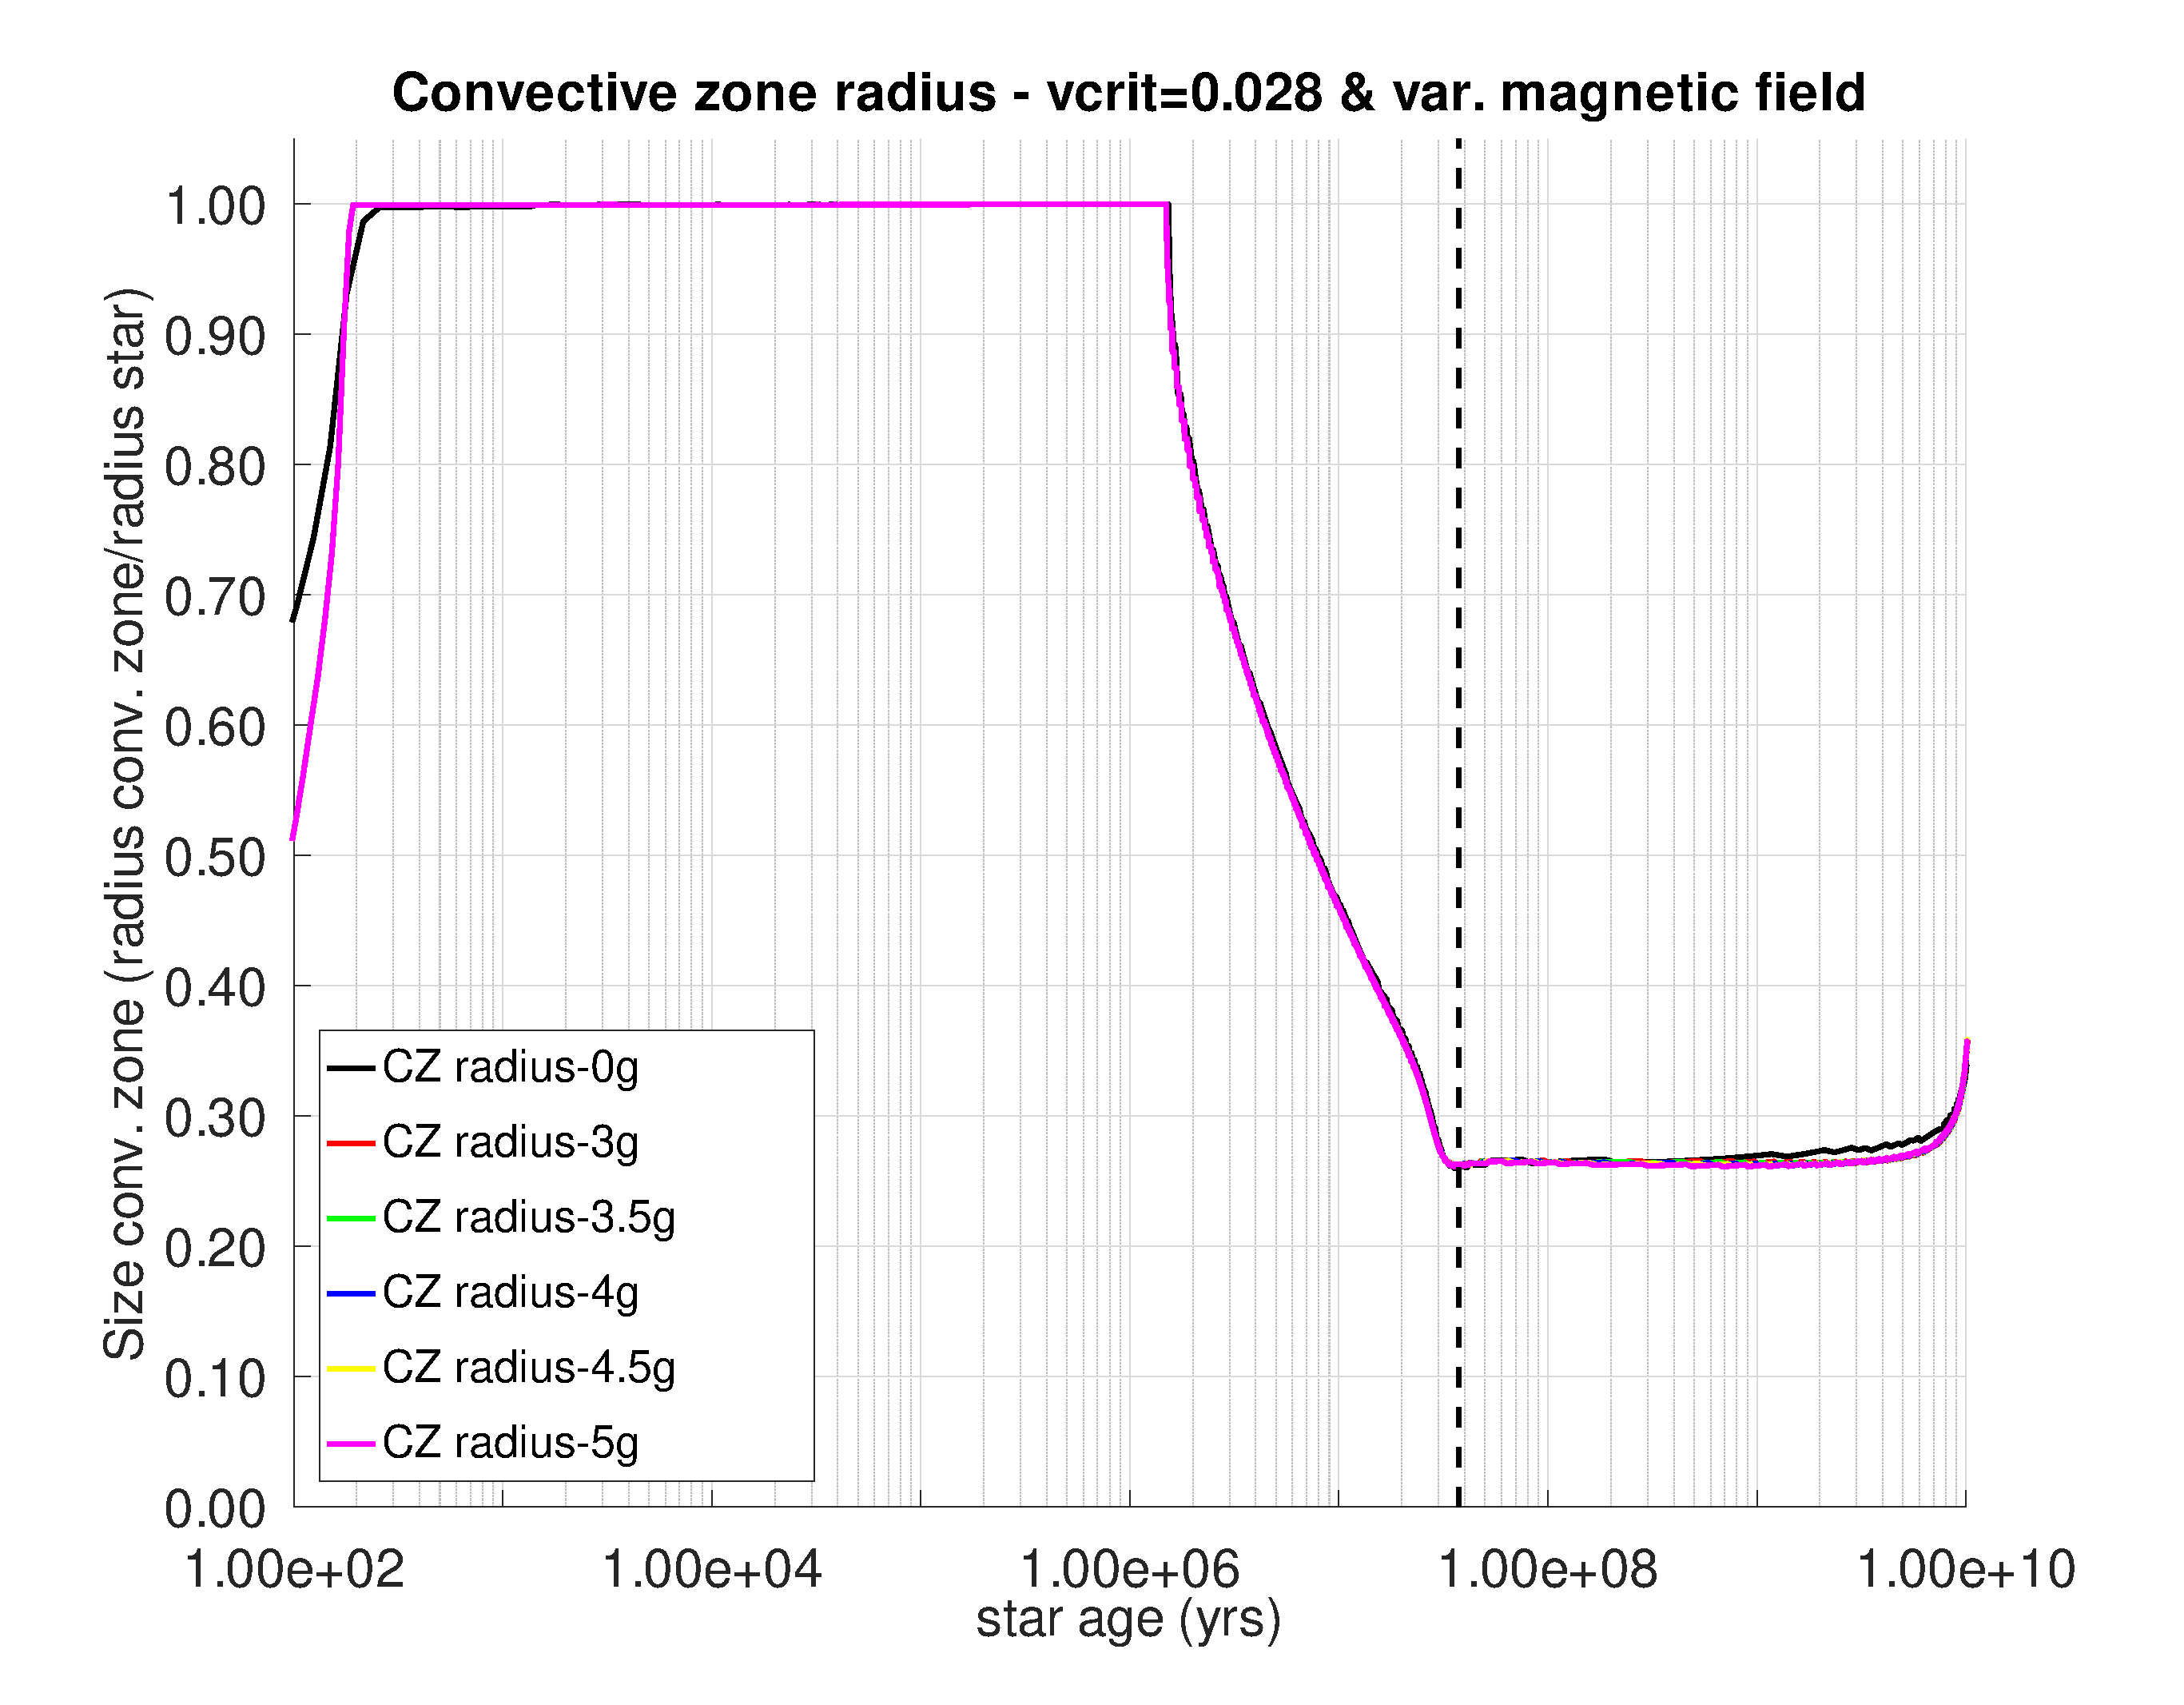
\includegraphics[trim = 30mm 15mm 20mm 15mm, clip,width=\columnwidth]{figures/cz_vc_028_var_g.eps}
    \caption{The evolution of convective zone size as a function of time for several 1 $\msun$ models. The models were all initialized with $\oomegac=0.0336$ and magnetic field strengths vary between $0.0\,\Gauss$ and $5.0\,\Gauss$. The dashed lines make reference to the ZAMS.}
    \label{fig:cz_vc_028_var_b}
\end{figure}

\begin{figure}
	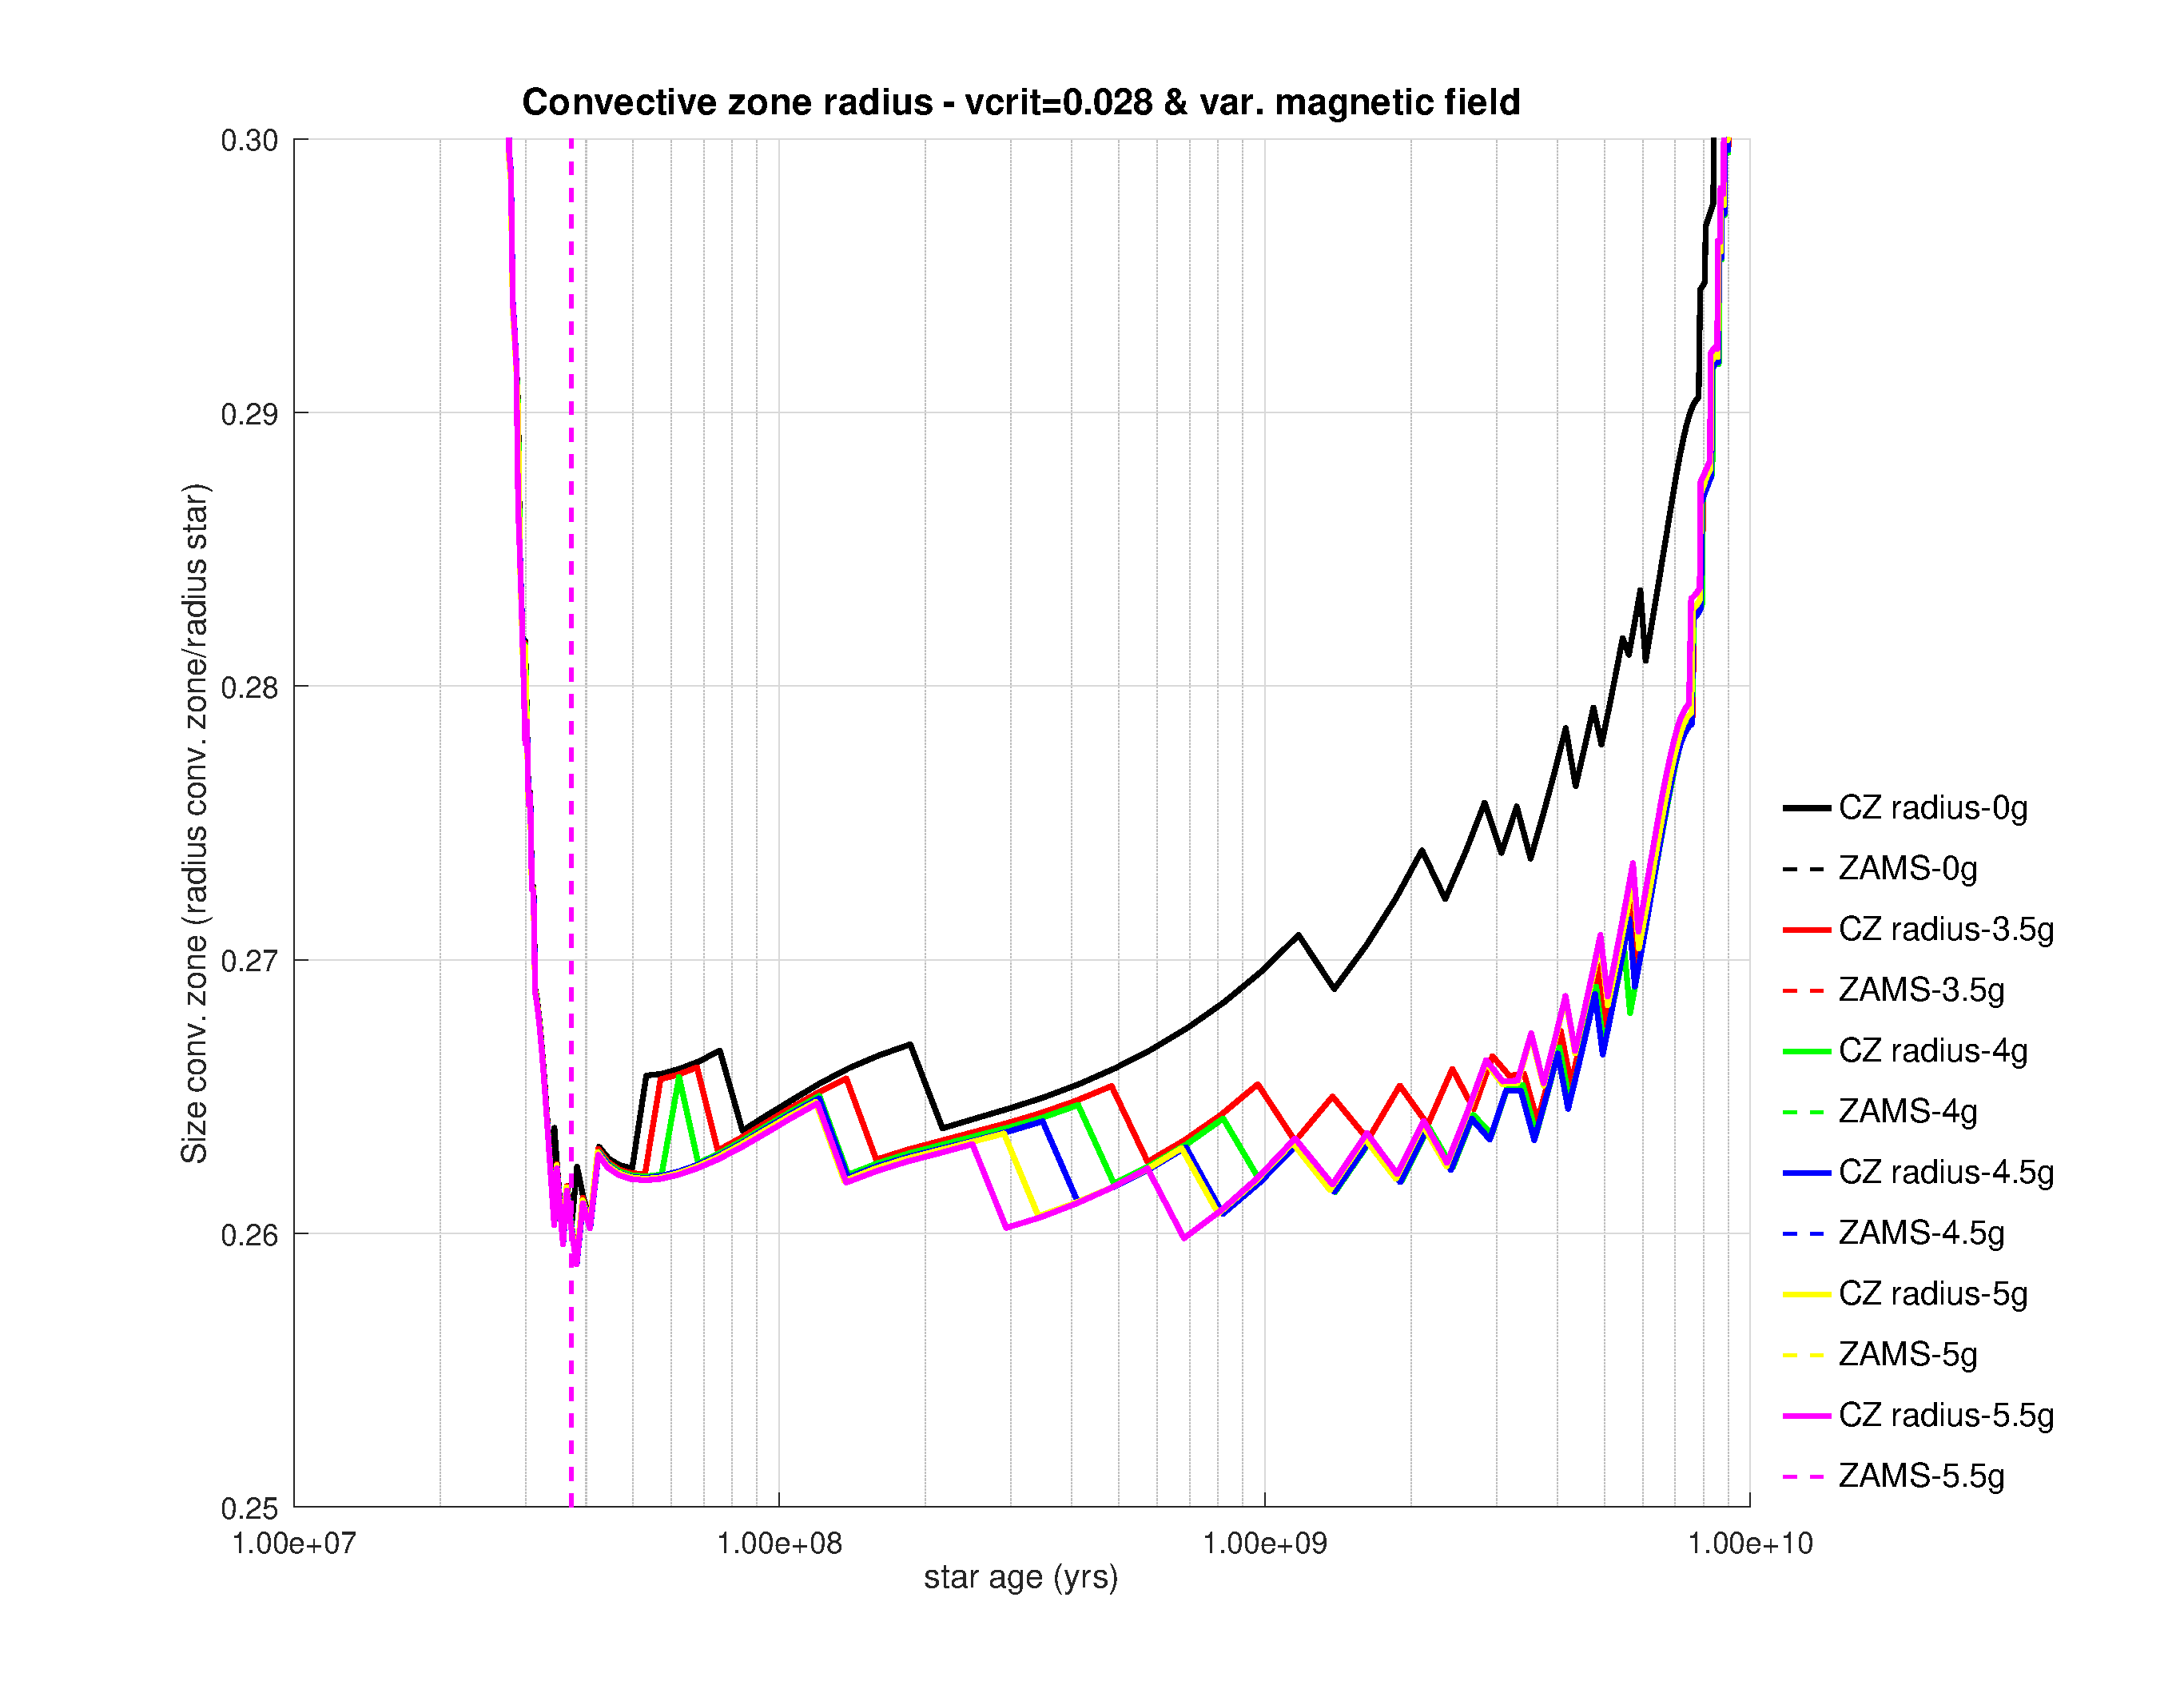
\includegraphics[trim = 30mm 15mm 20mm 15mm, clip,width=\columnwidth]{figures/cz_vc_028_var_g_z1.eps}
    \caption{Similar to Figure \ref{fig:cz_vc_028_var_b} but now showing in detail the convection zone size from the near ZAMS till the TAMS. As the intensity of the magnetic field increases, the size of the convective zone decreases.}
    \label{fig:cz_vc_028_var_b_z1}
\end{figure}

In Figure \ref{fig:mdot_vc_028_var_b} we can see the evolution of $\Dot{M}$ during PMS and MS for several 1 $\msun$ models. The models were all initialized with $\oomegac=0.0336$ and magnetic field strengths varying between $0.0\,\Gauss$ and $5.0\,\Gauss$. In the first stages of PMS is where the greatest mass loss is concentrated and this diminishes as it approaches the ZAMS. If we add to this scenario the fact that the star also decreases its radius during the PMS we have as result that the star increases $\Omega$ obeying the principle of conservation of AM. When reaching the ZAMS, the radius of the star remains more or less stable for much of the MS (except for its final stage) but continues to lose mass so it also increases its $\Omega$, although in a less aggressive way if we compare it with the PMS. However, as a consequence of both the appearance of the radiative core during Henyey track and the existence of a CZ (see Figure \ref{fig:mb_act_var_vel_vc_028}), the MB routine is activated, causing the angular velocity of the star to begin to decrease along the entire MS. The more intense the magnetic field, the greater the braking effect.\par 

\begin{figure}
	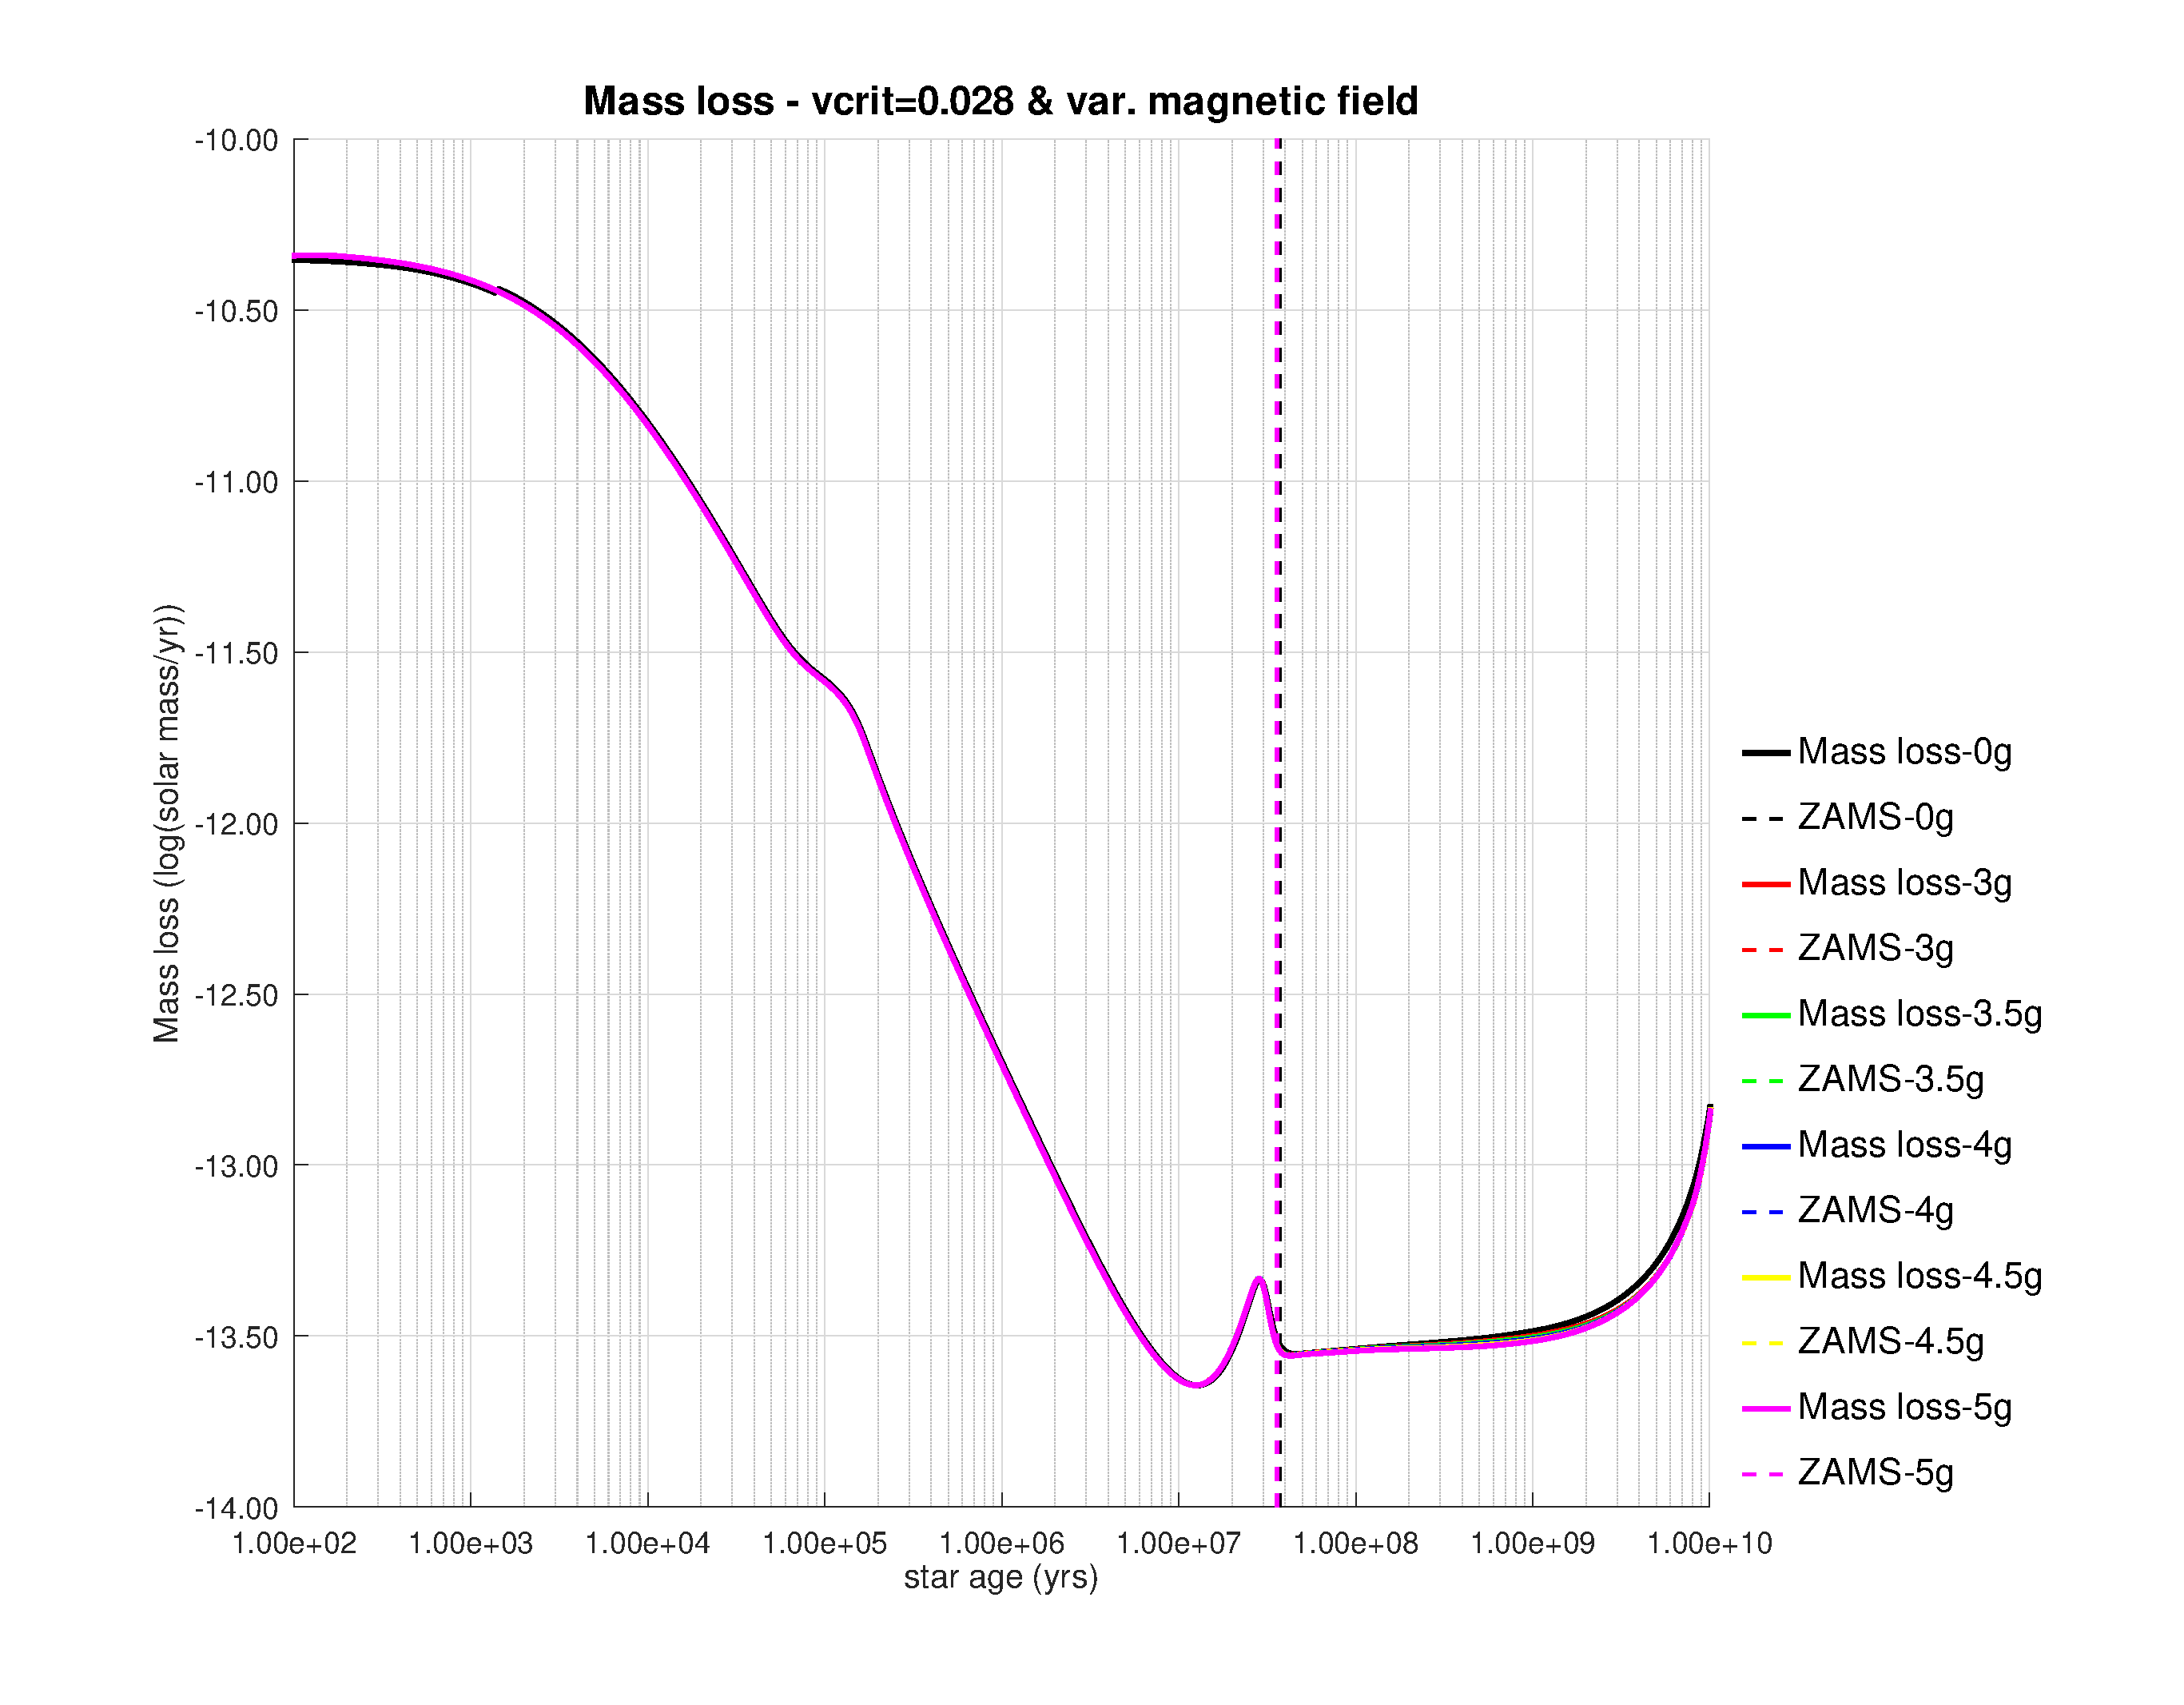
\includegraphics[trim = 30mm 15mm 20mm 15mm, clip,width=\columnwidth]{figures/mdot_vc_028_var_g.eps}
    \caption{The evolution of mass loss $\Dot{M}$ as a function of time for several 1 $\msun$ models. The models include different magnetic field intensity between $0.0\,\Gauss$ and $5.0\,\Gauss$ and PMS rotation with $\oomegac=0.028$. The dashed lines make reference to the ZAMS.}
    \label{fig:mdot_vc_028_var_b}
\end{figure}

\begin{figure}
	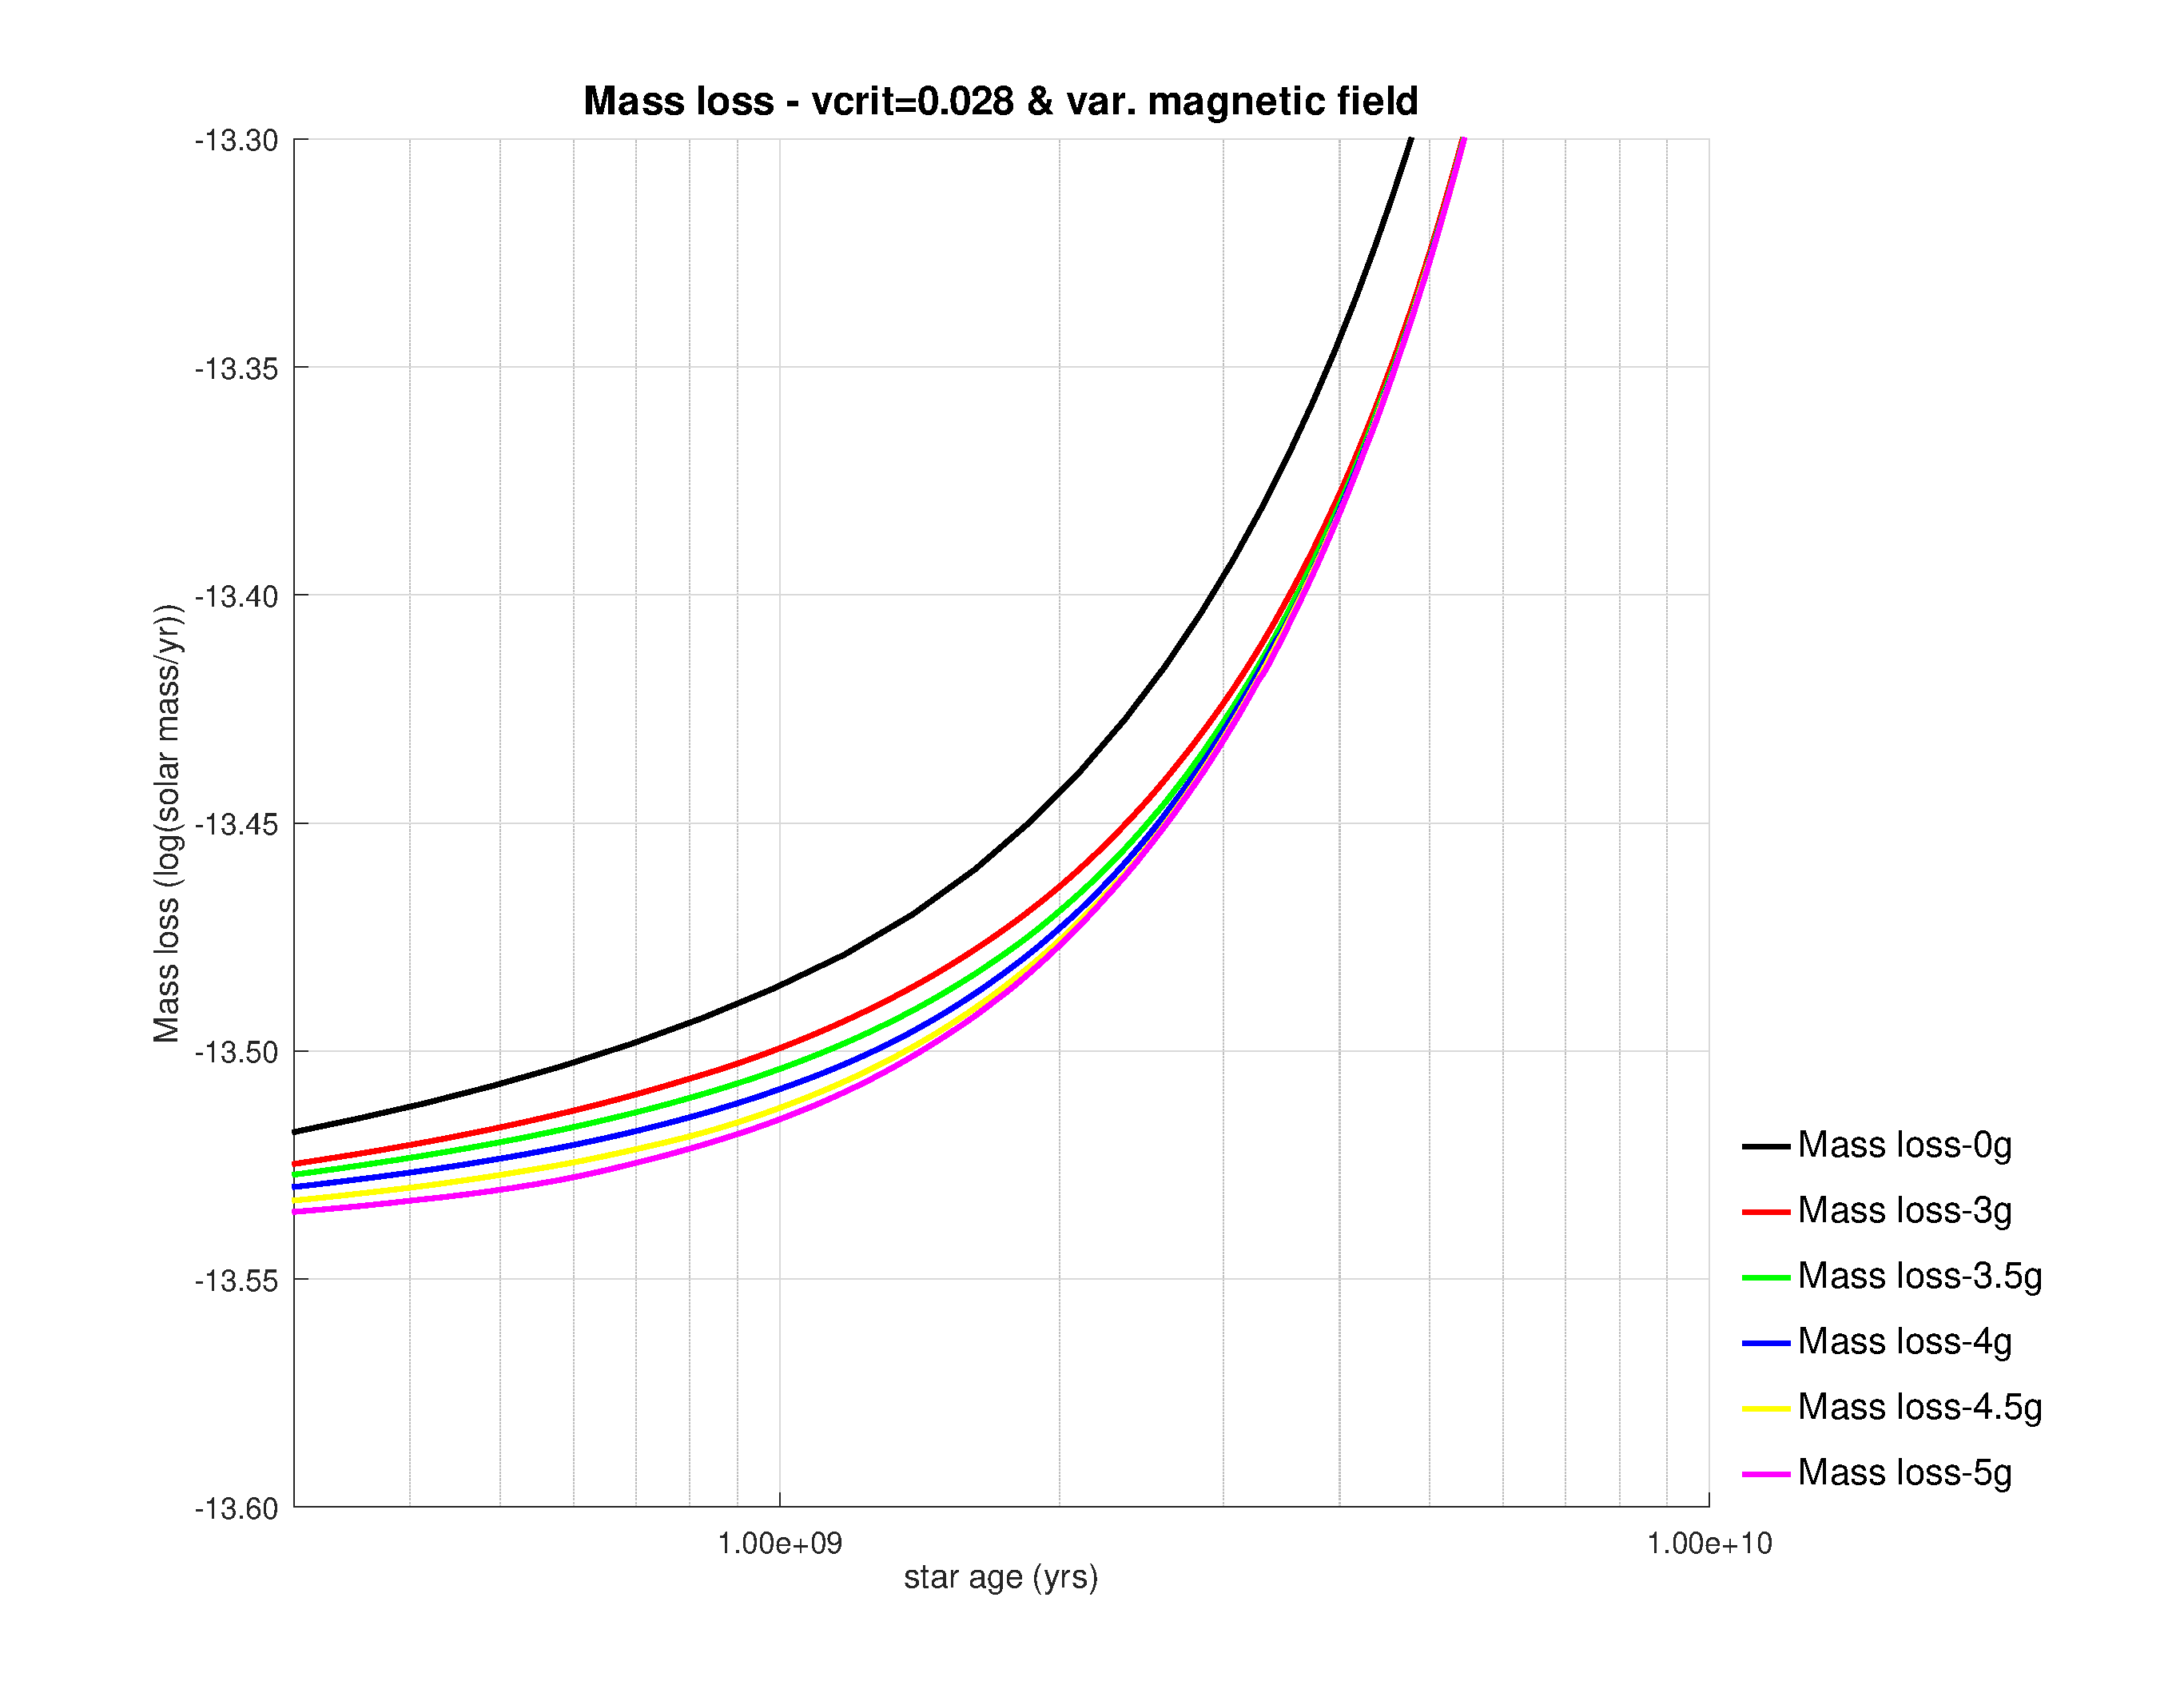
\includegraphics[trim = 30mm 15mm 20mm 15mm, clip,width=\columnwidth]{figures/mdot_vc_028_var_g_z1.eps}
    \caption{The evolution of mass loss $\Dot{M}$ as the star is approaching TAMS, as a function of time for several 1 $\msun$ models. The models include a variable magnetic field intensity between $0.0\,\Gauss$ and $5.0\,\Gauss$ and PMS rotation with $\oomegac=0.028$. The stronger the magnetic field, the lower $\Dot{M}$.}
    \label{fig:mdot_vc_028_var_b_z1}
\end{figure}

\begin{figure}
	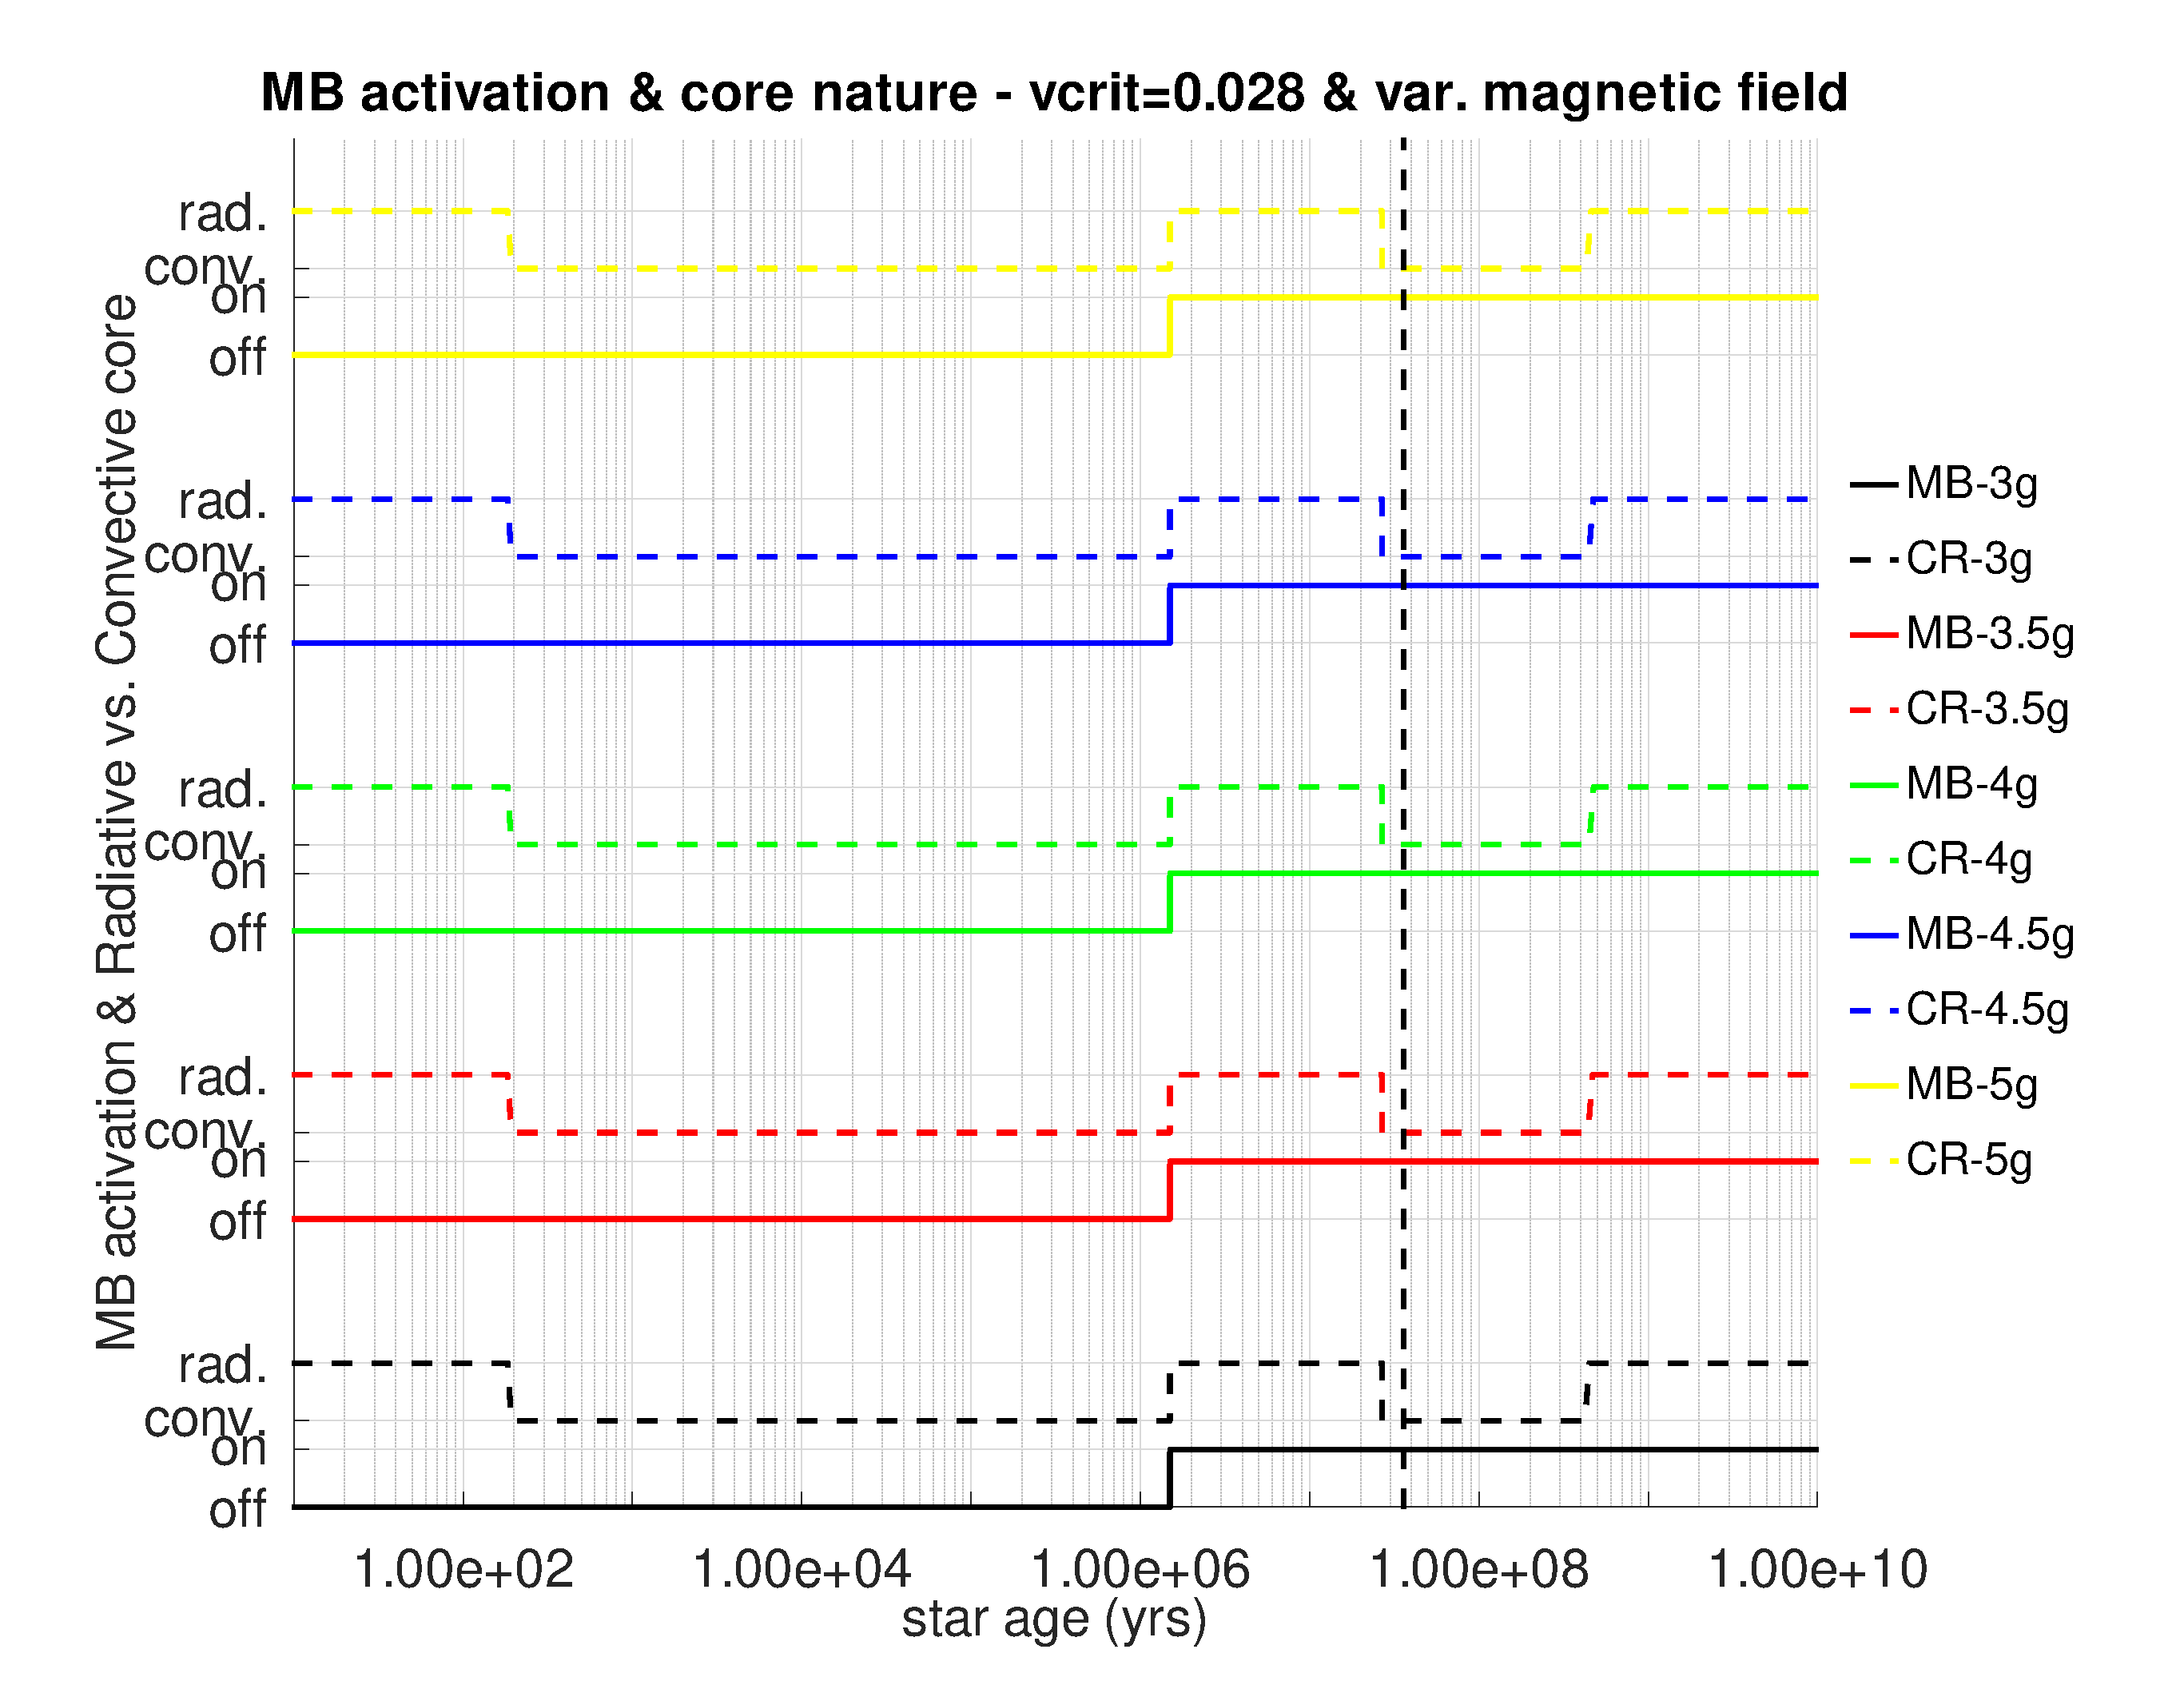
\includegraphics[trim = 30mm 15mm 15mm 15mm, clip,width=\columnwidth]{figures/mb_act_vc_028_var_g.eps}
    \caption{The activation of the magnetic braking routine as a function of the presence of a radiative core. The models include a magnetic field with an intensity ranging between $3.0\,\Gauss$ and $5.0\,\Gauss$ and PMS rotation with $\oomegac=0.0228$. The solid lines signal the magnetic braking routine activation (on) and deactivation (off). The horizontal dashed lines inform about the star's core nature: radiative (rad) or convective (conv). By implementation decision, once the routine is activated, it remains on even if the star's core nature change to convective. The vertical dashed lines make reference to the ZAMS.}
    \label{fig:mb_act_var_vel_vc_028}
\end{figure}

\subsection{Alternative Li evolution with MB}
Up to this point, the simulations of the different models have been based on the parameterization gathered in table \ref{tab:phy_mesa}, which in turn has been adopted from \citet{Choi2016}. If we recall the evolution of the Li shown in Figures~\ref{fig:li_var_vel_0g} and \ref{fig:li_var_vel_4_0g}, we highlighted that on both cases too much Li was burned before reaching the ZAMS and therefore do not match with the Pleiades average surface Li abundance. On the other than, using a parameterization slightly different from the one used until now in which the parameters of convection and overshooting have been readjusted according to table \ref{tab:phy_alt_mesa}, the simulations can reproduce more faithfully both the Li abundance of the Pleiades cluster and of the Sun (see Figure \ref{fig:li_3_0g_0314vc}).\par

\begin{table}
	\centering
	\caption{Alternative MTL and overshooting parameters.}
	\label{tab:phy_alt_mesa}
	\begin{tabular}{ll} 
		\hline
		Parameter & Adopted prescriptions and values\\
		\hline
		Convection & MLT + Ledoux, $\alpha_\mathrm{MLT}$ = 1.70\\
		Overshoot & time-dependent, diffusive, $f_\mathrm{ov,core}=0.016$, \\ & $f_\mathrm{ov,sh}=0.002$\\
		\hline
	\end{tabular}
\end{table}


\begin{figure}
	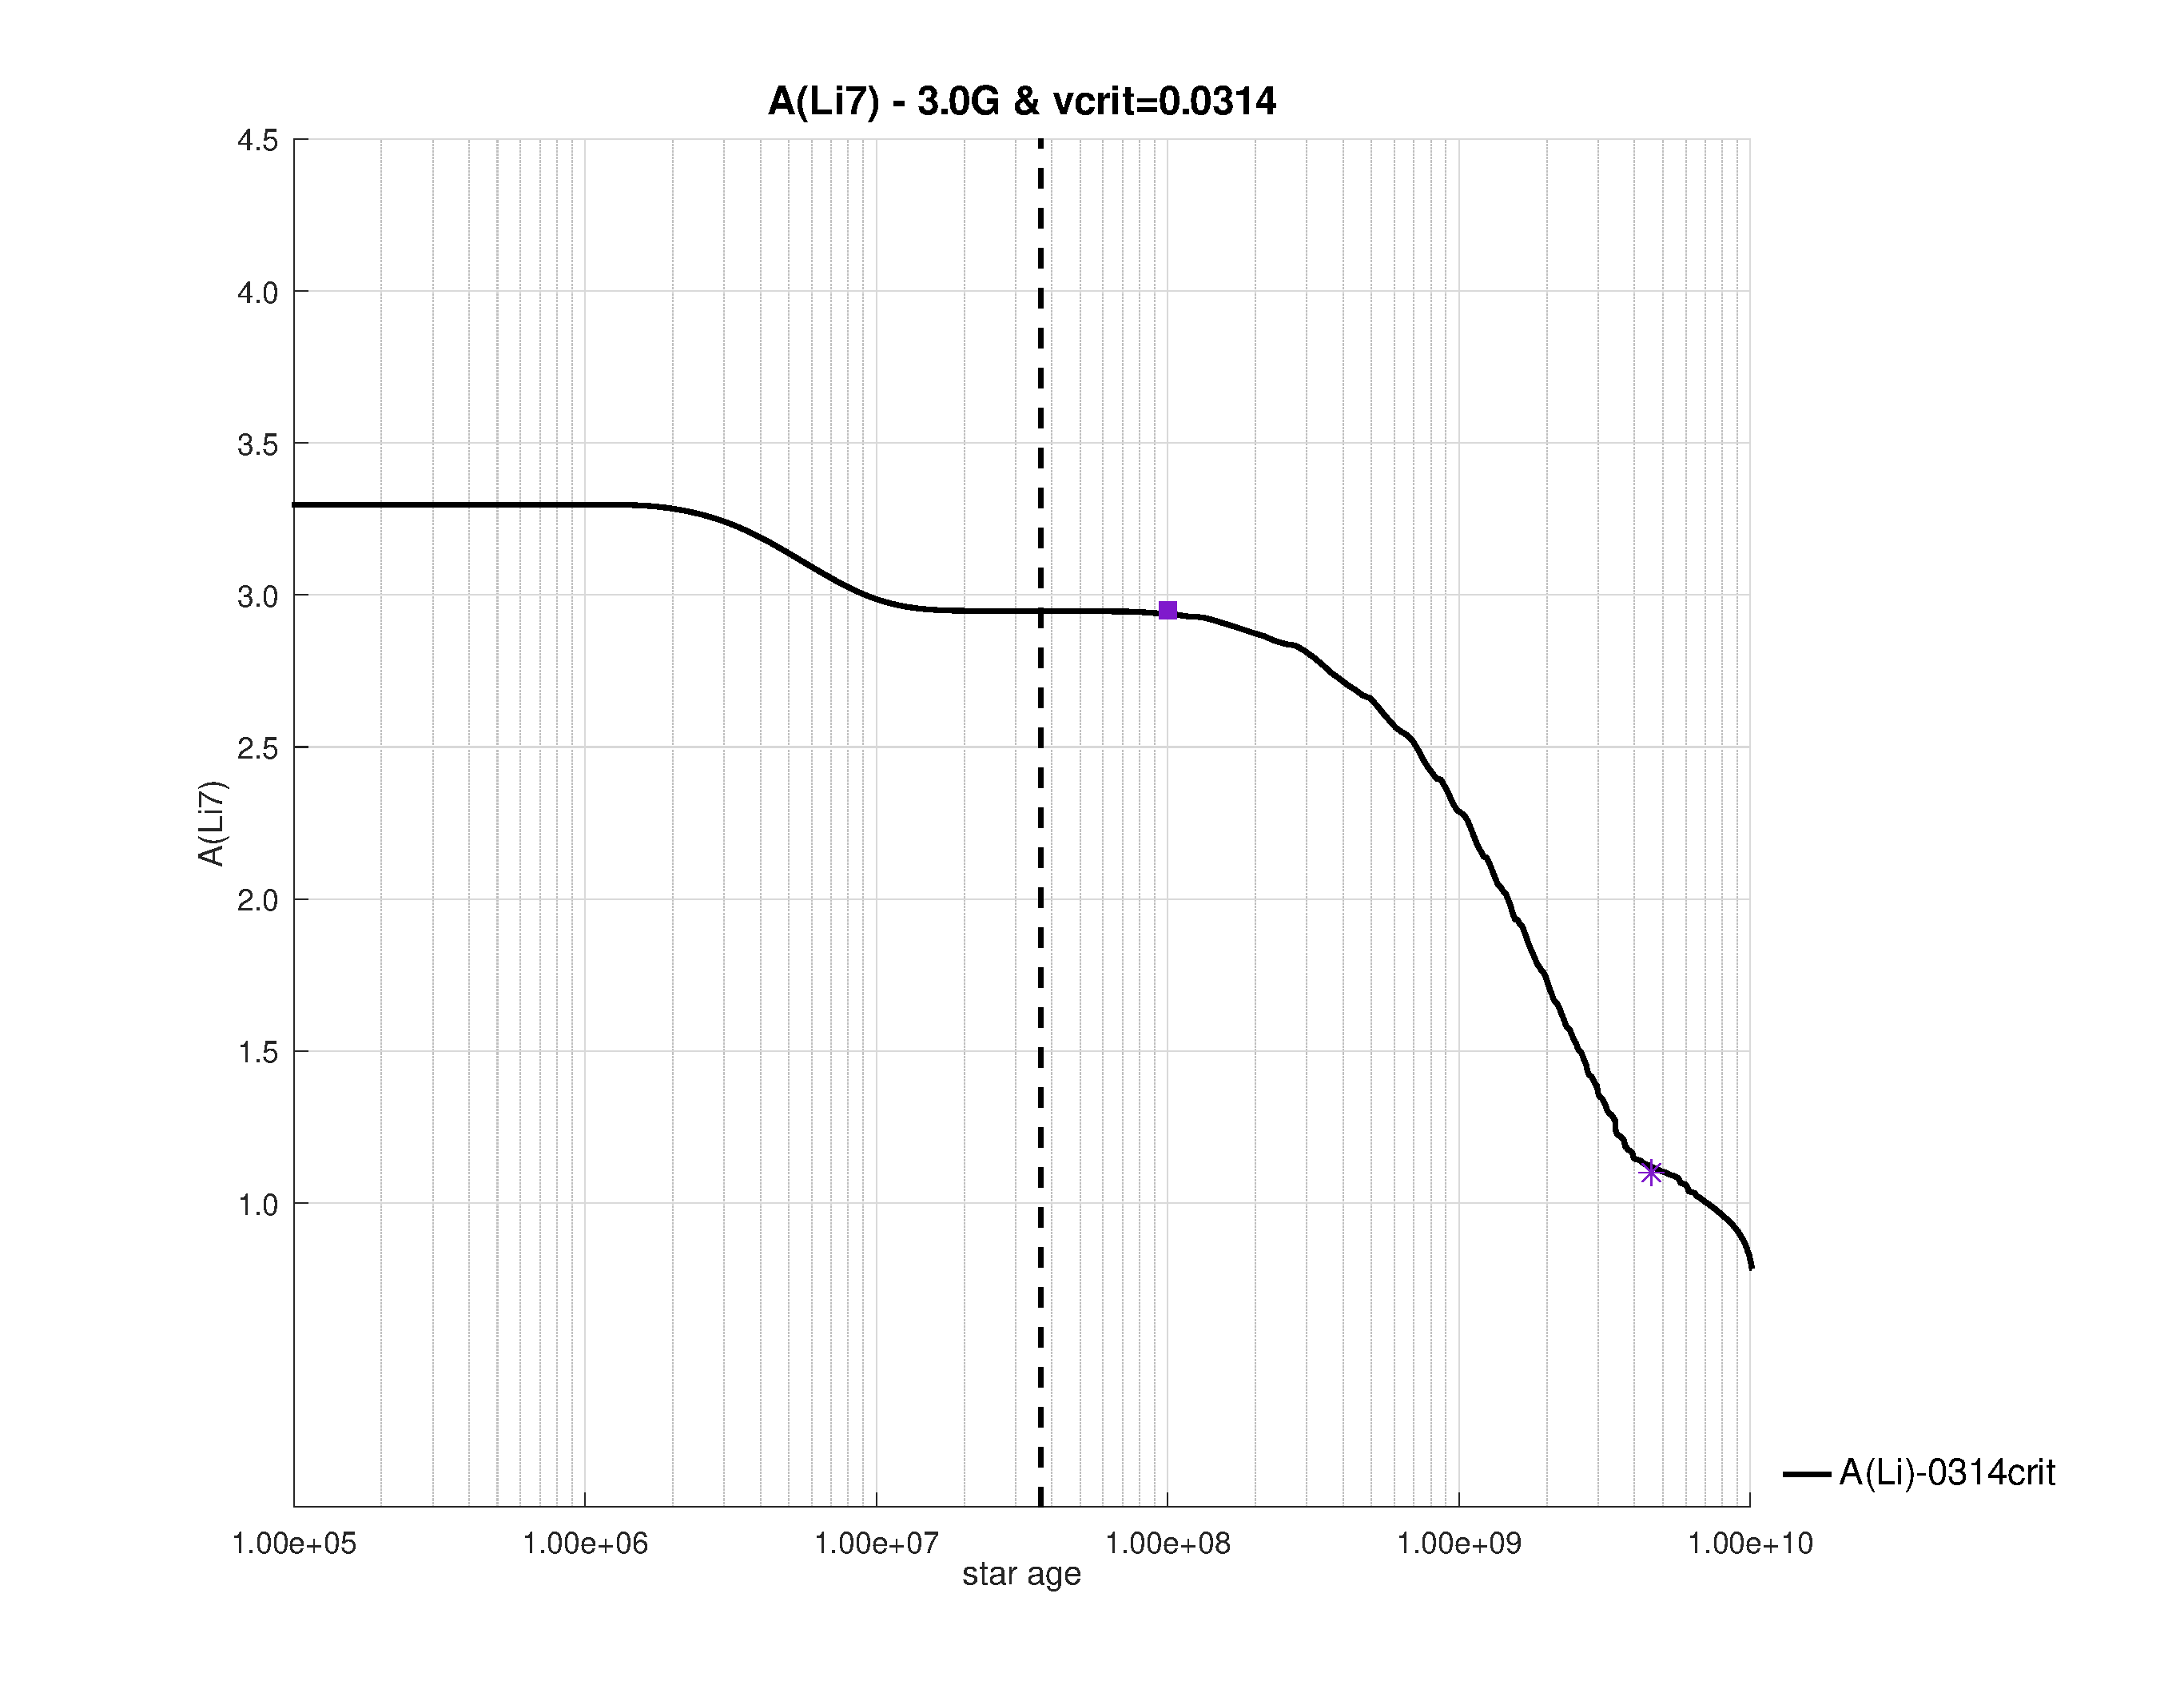
\includegraphics[trim = 35mm 15mm 20mm 15mm, clip,width=\columnwidth]{figures/li_3_0g_0314vc.eps}
    \caption{The evolution of surface \isotope[7]{Li} abundance relative to \isotope[1]{H}, as a function of time for a 1 $\msun$ model. The model include a magnetic field with an intensity of 3\,G and PMS rotation with $\oomegac= 0.0314$, respectively. MLT and overshooting parameters have been set to $\alpha_\mathrm{MLT}=1.70$, $f_\mathrm{ov,core}=0.016$, $f_\mathrm{ov,sh}=0.002$. The purple star and square are surface Li abundance for the present-day Sun \citep{Asplund2009} and the Pleiades cluster \citep{Sestito2005} respectively. The dashed lines make reference to the ZAMS.}
    \label{fig:li_3_0g_0314vc}
\end{figure}

Similarly, the evolution of the angular velocity for this new configuration is shown in Figure \ref{fig:rot_vel_var_vel_mlt_3_0g}. Here, on the contrary, we have to note that with the new simulation we still do not reproduce correctly the angular velocity of the Sun. Having said this and based on the results obtained in this last section, it becomes evident that the influence of the free, relatively arbitrary, parameters associated with Mixing Lenght Theory (MLT) significantly condition the evolution of the abundance of Li. This opens the door for other solar-compatible parameterizations to offer results in line with the observations in young stellar clusters and for the Sun. \par

\begin{figure}
	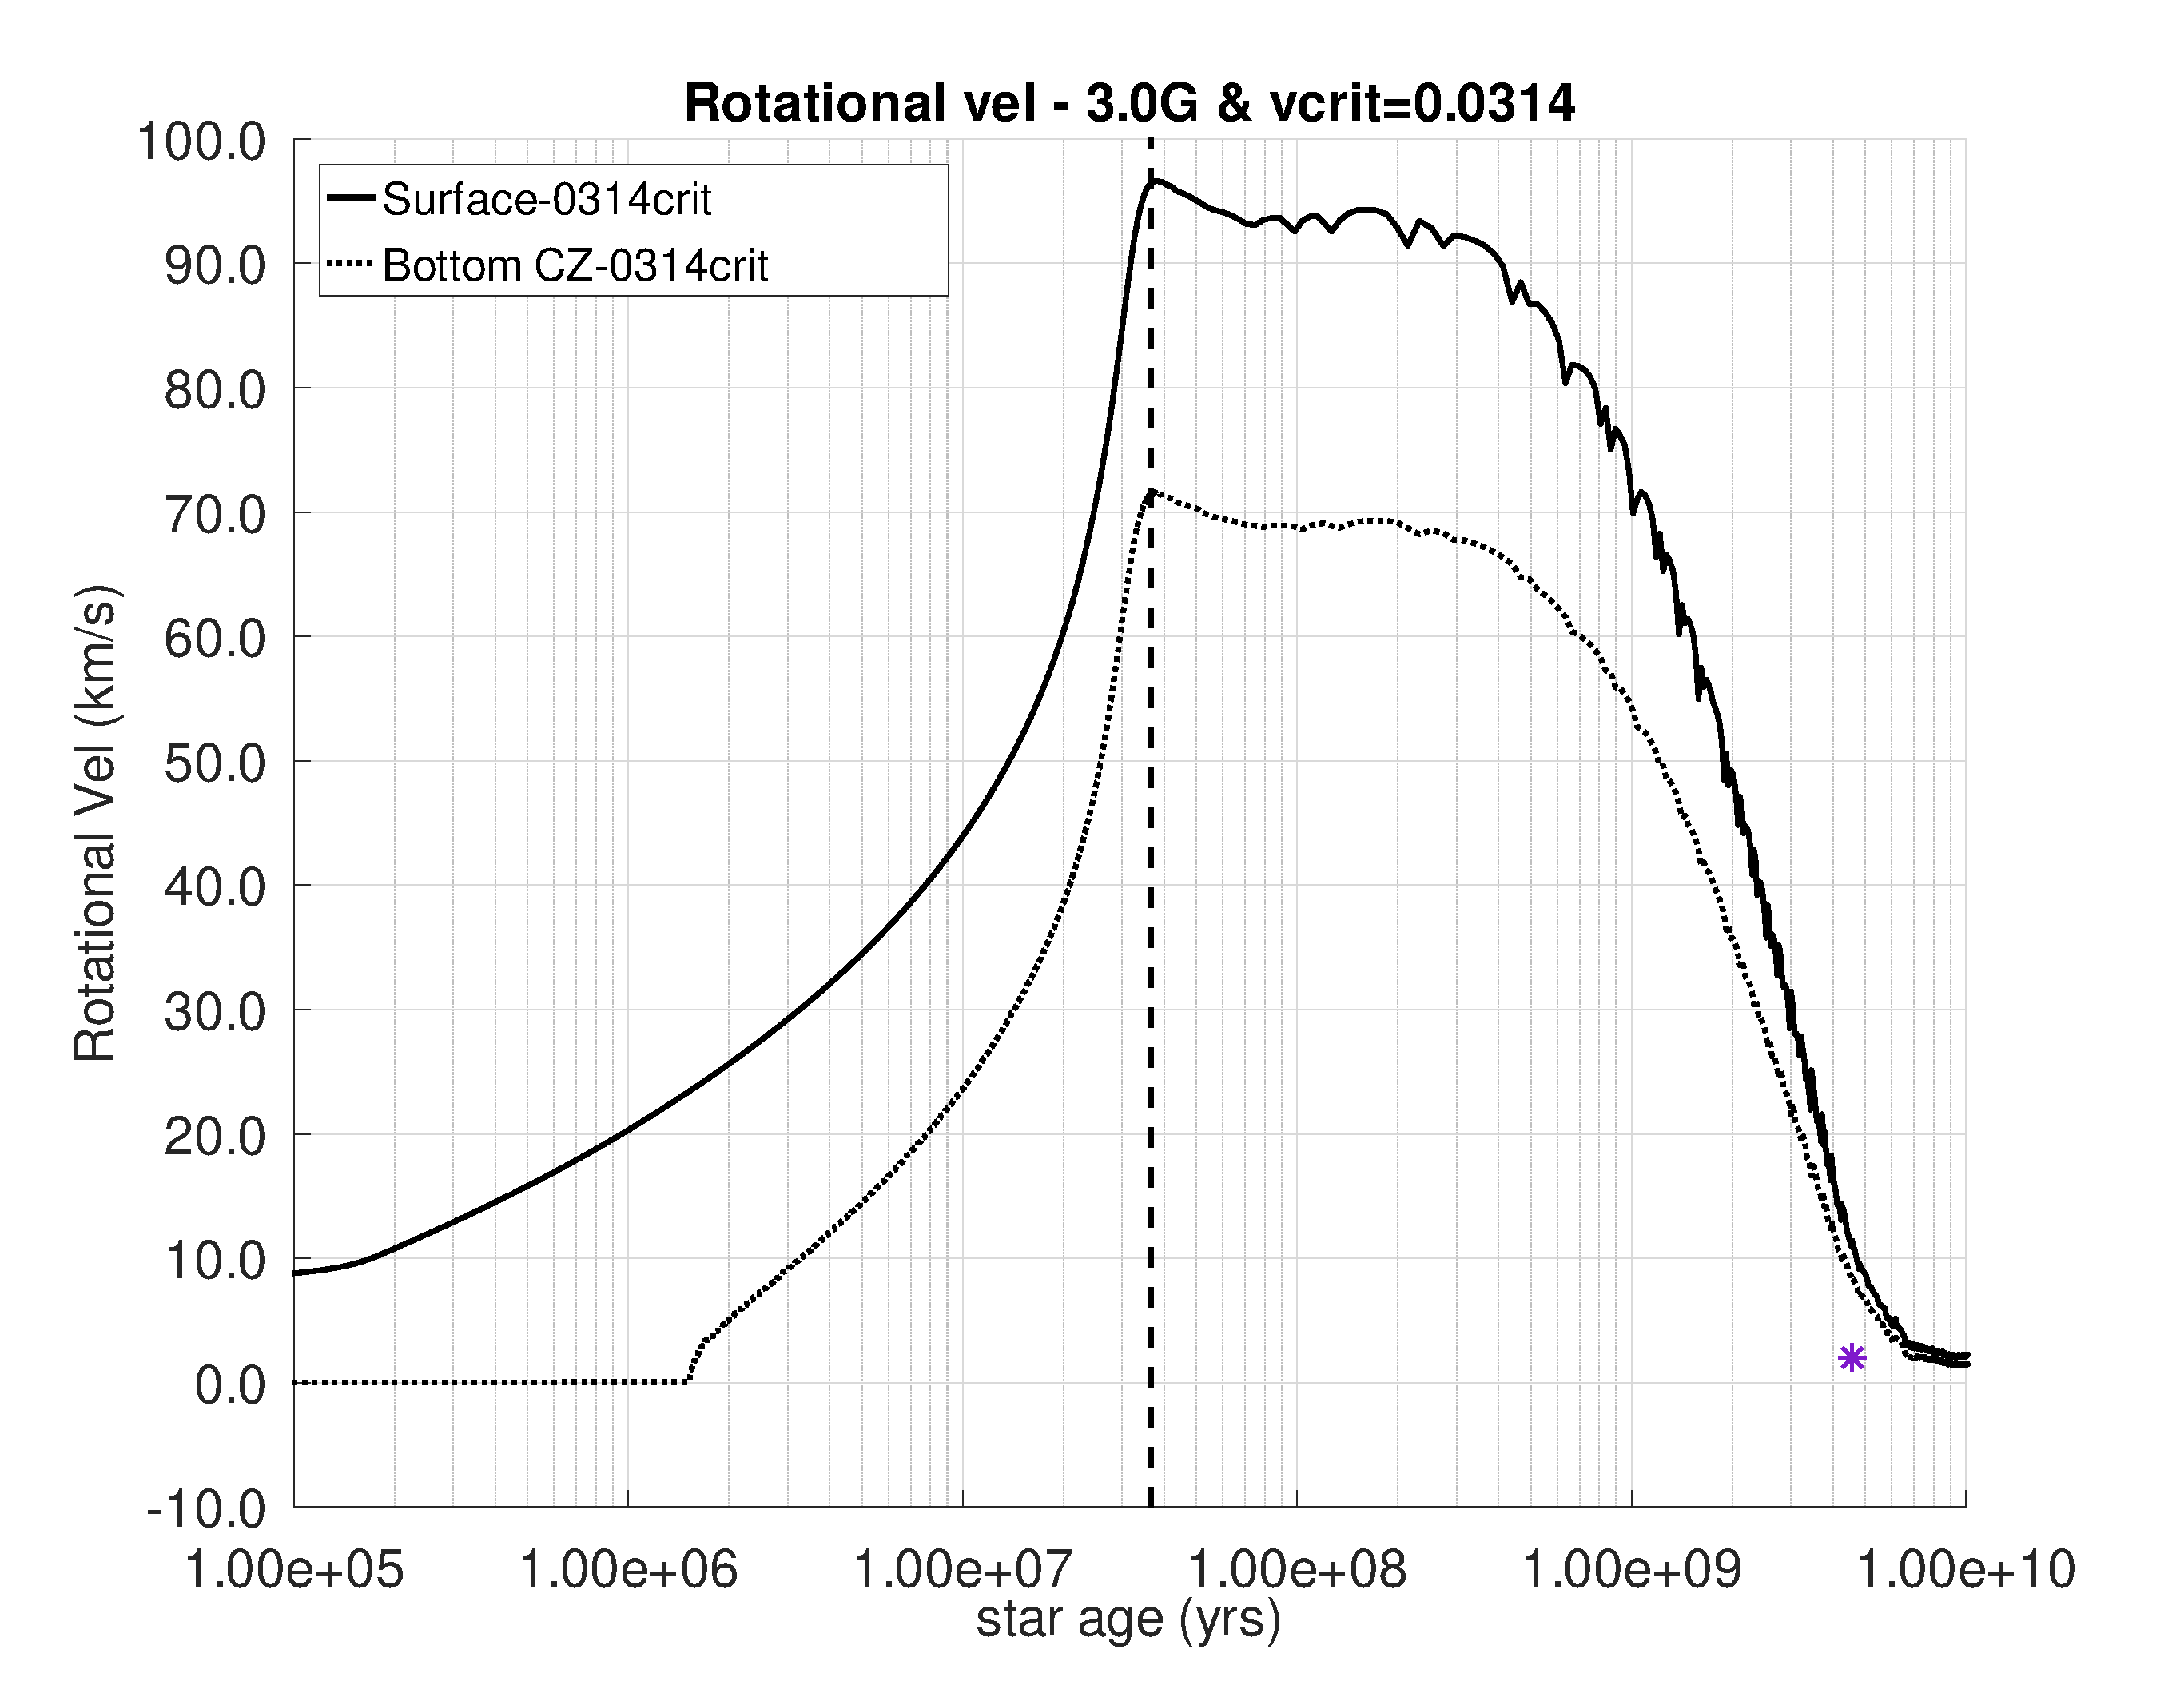
\includegraphics[trim = 30mm 15mm 20mm 15mm, clip,width=\columnwidth]{figures/rot_vel_3_0g_0314vc.eps}
    \caption{The evolution of surface rotational velocity, as a function of time for a 1 $\msun$ model. The model include a magnetic field with an intensity of 3\,G, PMS rotation with $\oomegac=0.0314$, respectively and MB. MLT and overshooting parameters have been set to $\alpha_\mathrm{MLT}=1.70$, $f_\mathrm{ov,core}=0.016$, $f_\mathrm{ov,sh}=0.002$. The purple star is the surface angular velocity for the present-day Sun \citep{Gill2012}. The dashed lines make reference to the ZAMS.}
    \label{fig:rot_vel_var_vel_mlt_3_0g}
\end{figure}

We propose that this adjustment could also potentially be achieved by a law of interdependence between $\Omega$ and $B$. So that, during the PMS, when the star rotates faster, the MB effect is more efficient. On the other hand, during the MS, when the start slows down, the MB will become less intensive. This approach would establish a self-regulating mechanism over the angular velocity of the star that would end up directly influencing the evolution of A(Li). This is the line of work in which we will continue our research.\par


\section{Conclusions and future works} \label{sec_4}
We have demonstrated that both rotation and MB induced effects must be taken into account in the theoretical models for a proper understanding and modelling of the evolution of stars. The latter is of major importance both for the transport of AM and for the transport of chemical elements. We are also well aware that we are still far from understanding the exact physical mechanisms that govern these processes, so it is necessary to continue to delve into these areas of study. Particularly the study of the evolution of the magnetic fields during the PMS and MS and their impact on AML. Future and improved implementations of our routine will be made to study the results on tracks, surface Li composition, rotation, etc. It is likely that in a rotating stellar model simulated with MB from the beginning, the differential rotation is very much reduced and therefore Li abundances observed in young stars could be properly explained. It is equally important to understand better the general role of mass loss in AML and mostly in cooler, low-mass stars. Nowadays it is challenging to determine the terminal velocity of the stellar wind for this type of stars which, as documented previously, plays a key role on the AML.\par

We emphasize as well that our models fail to match the observed solar Li abundance and $\Omega$. We cannot, therefore, ascertain to have correctly modeled the rotational history of the Sun. Therefore, in view of these shortcomings in our models, we must analyse the results obtained with caution and not draw any premature conclusions. Having said that, we have also shown how an alternative MLT parametrizations could produce results in line with the observations. We are convinced that our research is on the right track and we do believe that the following conclusions, based on the results described in previous sections, have been sufficiently supported in the course of this work:
\begin{enumerate}
    \item Inclusion of the magnetic field leads to cooler models and lower Li depletion in the MS.
    \item A combination of rotation during the PMS and MB effect during MS produces different, potentially more promising behavior than those produced by standard models.
    \item $\teff$ from standard evolutionary tracks represent upper limits since these models do not take into consideration the magnetic braking effect nor rotation.
    \item The convective zone extension decreases when the intensity of the magnetic field increases.
    \item MB during PMS and/or adjustment of MLT overshooting and $\amlt$ free parameters seems to be also required for explaining Li abundances in young clusters.
\end{enumerate}

In the near future, with the new version of our code including magnetic field evolution in MESA, we will focus our efforts on understanding how magnetic fields are linked to rotation, how their topologies are and how they evolve in time in order to go beyond the treatment on the MB routine that has been done in this work.\par



\section*{Acknowledgements}
We are pleased to acknowledge Jieun Choi her kindness in responding to the different questions about her work which were aimed to reproduce the results obtained as far as Li is concerned, and also for allowing us access to the MESA files she used. Also we very much appreciate the expert support provided by Elisa Delgado-Mena during the process review of this document. Similarly, we wish also to thank Matteo Cantiello and Bill Paxton for their very valuable support in the development of the magnetic braking routine in MESA. Finally, we wish to acknowledge the generous work and help offered by the MESA community. Authors acknowledges funding support from Spanish public funds (including FEDER fonds) for research under projects ESP2017-87676-C5-2-R and ESP2017-87676-C5-5-R. JCS also acknowledges support from project RYC-2012-09913 under the 'Ram\'on y Cajal' program of the Spanish Ministry of Science and Education.

\section*{Software}
The simulations used in this paper been executed with the MESA release 10398 \footnote{\url{http://mesa.sourceforge.net/release/2018/03/21/r10398.html}}. The different figures have been generated making use of GNU Octave 5.1.0. \footnote{\url{https://www.gnu.org/software/octave/}} 

%%%%%%%%%%%%%%%%%%%%%%%%%%%%%%%%%%%%%%%%%%%%%%%%%%

%%%%%%%%%%%%%%%%%%%% REFERENCES %%%%%%%%%%%%%%%%%%

% The best way to enter references is to use BibTeX:

\bibliographystyle{mnras}
%\bibliography{magbrlitium} % if your bibtex file is called example.bib
\bibliography{mblithium}


% Alternatively you could enter them by hand, like this:
% This method is tedious and prone to error if you have lots of references
%\begin{thebibliography}{99}
%\bibitem[\protect\citeauthoryear{Author}{2012}]{Author2012}
%Author A.~N., 2013, Journal of Improbable Astronomy, 1, 1
%\bibitem[\protect\citeauthoryear{Others}{2013}]{Others2013}
%Others S., 2012, Journal of Interesting Stuff, 17, 198
%\end{thebibliography}

%%%%%%%%%%%%%%%%%%%%%%%%%%%%%%%%%%%%%%%%%%%%%%%%%%

%%%%%%%%%%%%%%%%% APPENDICES %%%%%%%%%%%%%%%%%%%%%

\appendix

\section{Mesh models visualization}
The following figures comprise a series of grids as a function of time and for several 1 $\msun$ models in which on the one hand, the evolution of surface \isotope[7]{Li} abundance relative to \isotope[1]{H} for both variable magnetic field intensities and angular velocities and on the other hand, the evolution of surface rotational velocity are shown.

\begin{figure*}
    \centering
    \begin{subfigure}[h]{0.47\textwidth}
    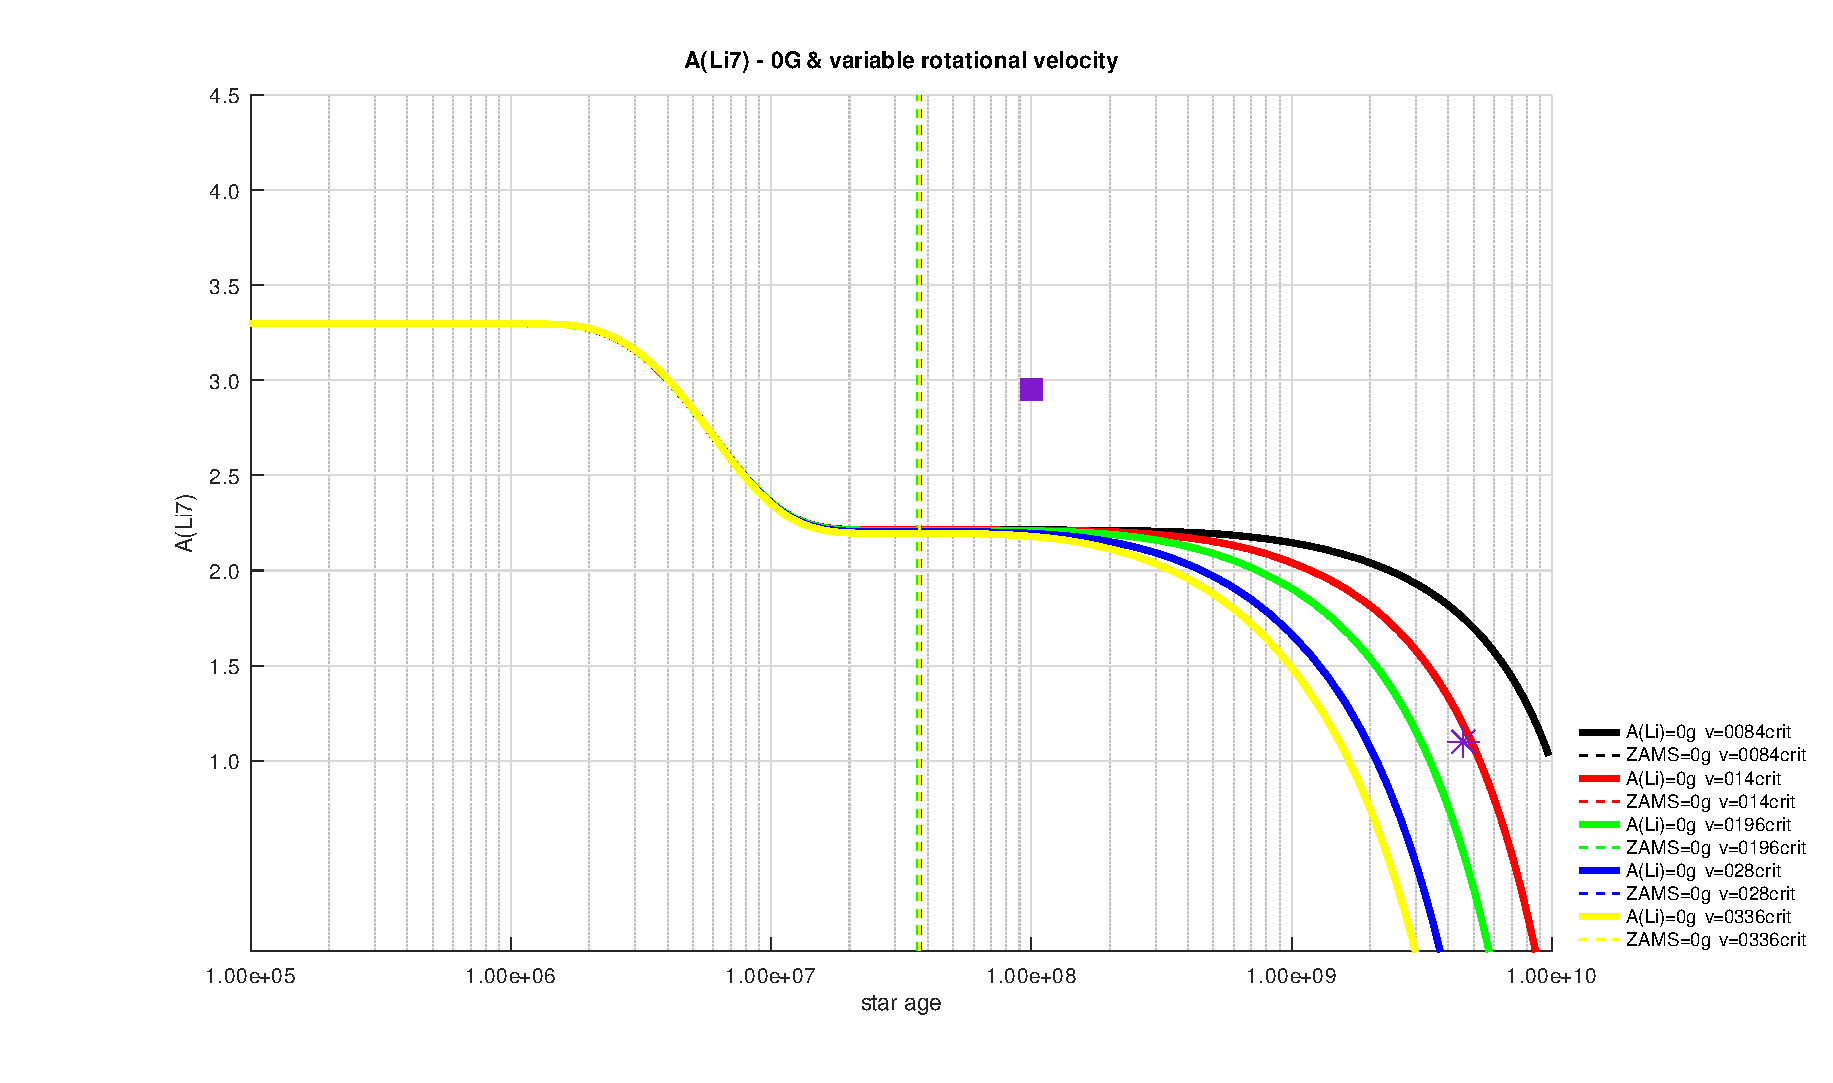
\includegraphics[trim = 35mm 15mm 20mm 15mm, clip,width=\textwidth]{figures/li_var_vel_0_0g.eps}
    \label{fig:subim1}
    \end{subfigure}
    \begin{subfigure}[h]{0.47\textwidth}
    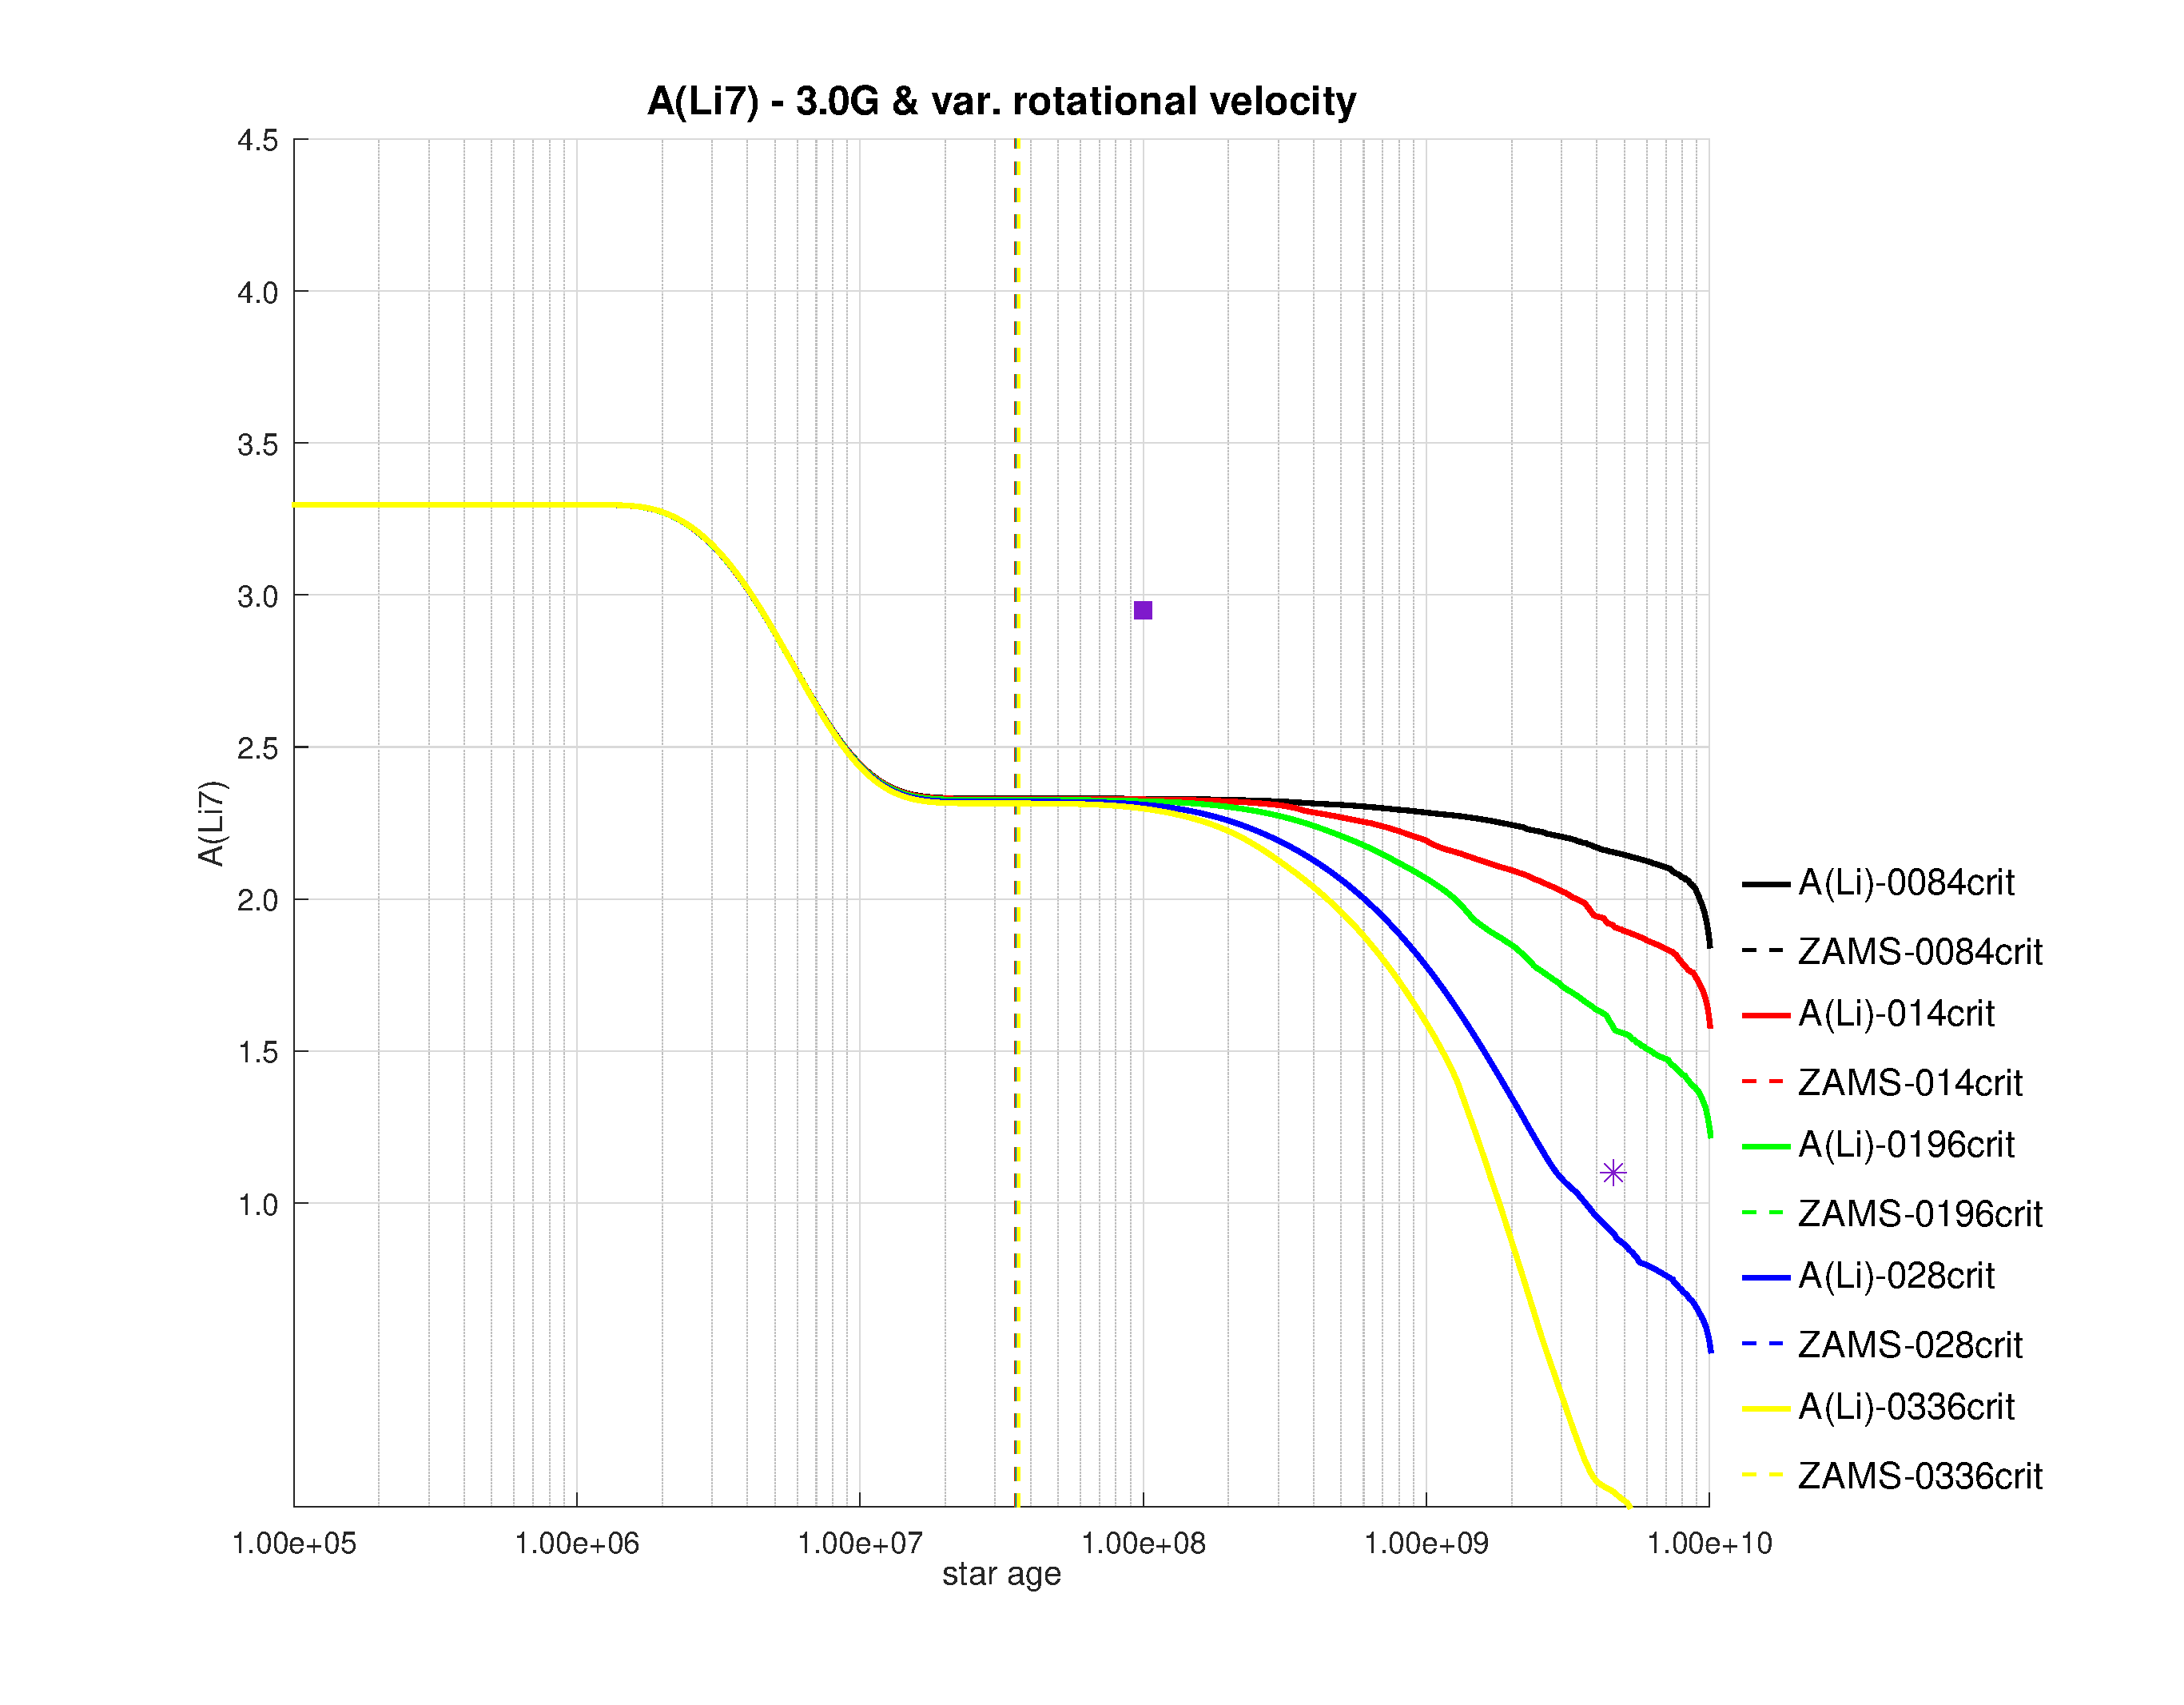
\includegraphics[trim = 35mm 15mm 20mm 15mm, clip,width=\textwidth]{figures/li_var_vel_3_0g.eps}
    \label{fig:subim2}
    \end{subfigure}
    \begin{subfigure}[h]{0.47\textwidth}
    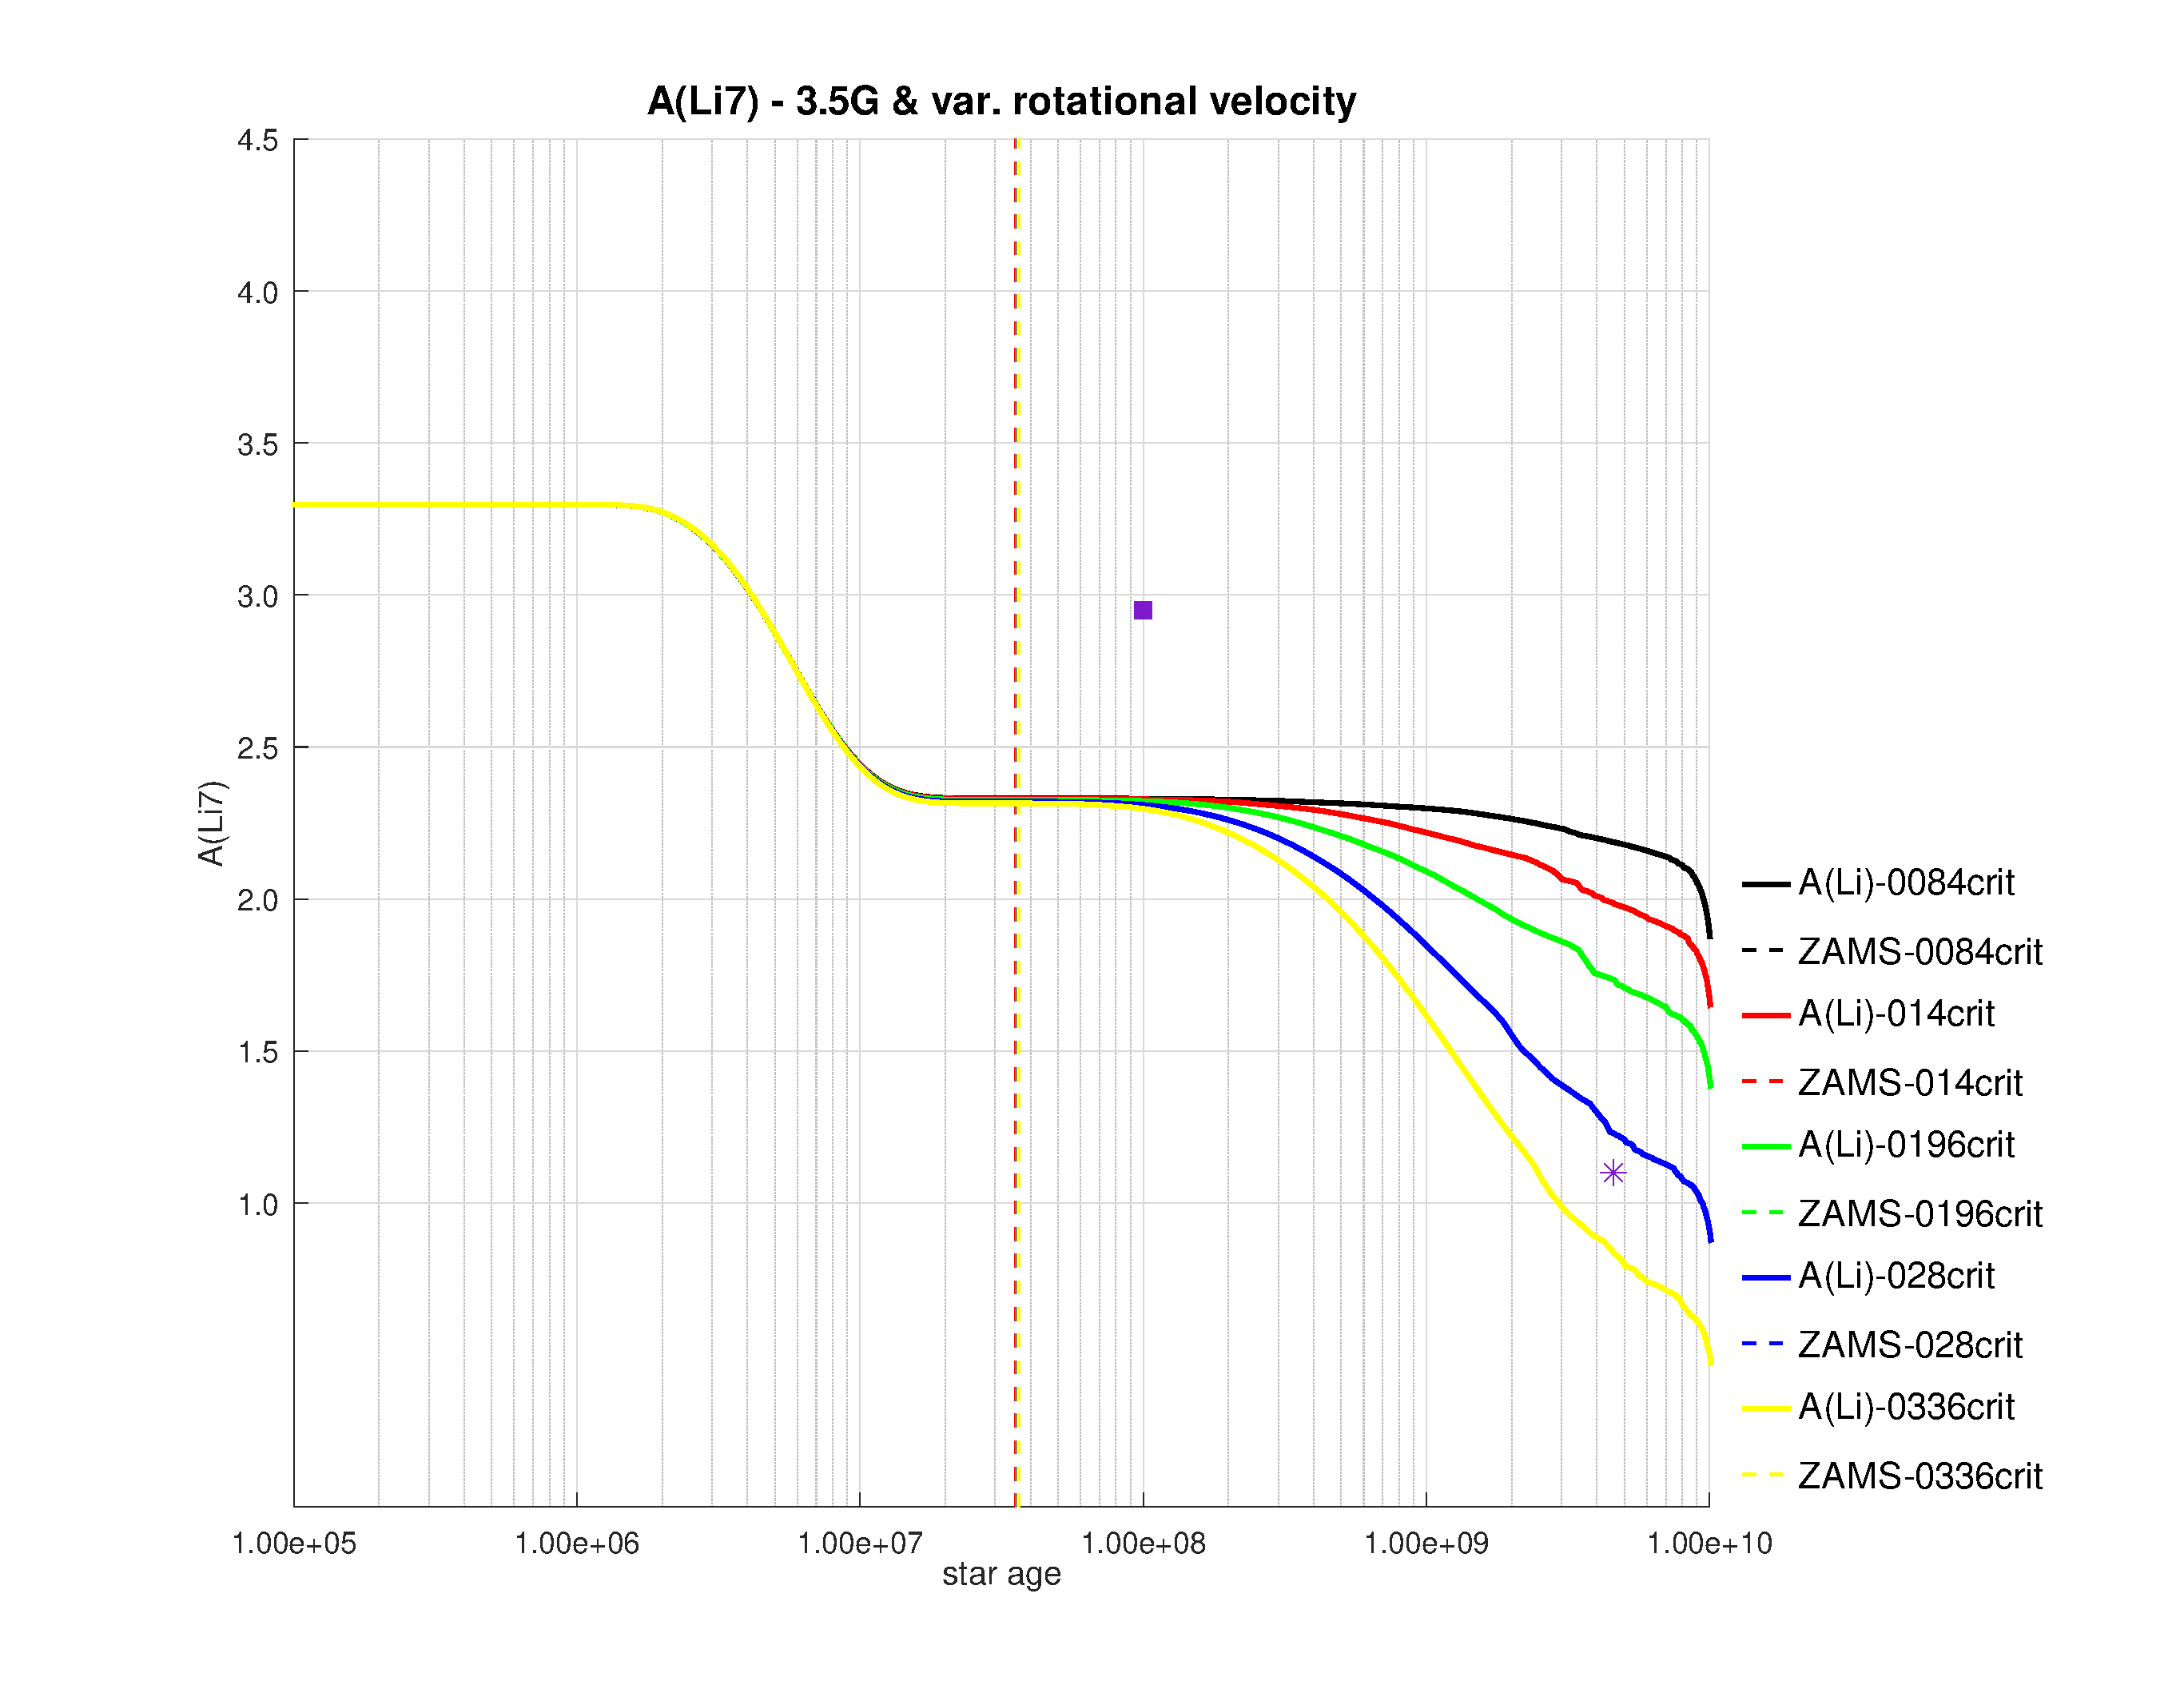
\includegraphics[trim = 35mm 15mm 20mm 15mm, clip,width=\textwidth]{figures/li_var_vel_3_5g.eps}
    \label{fig:subim3}
    \end{subfigure}
    \begin{subfigure}[h]{0.47\textwidth}
    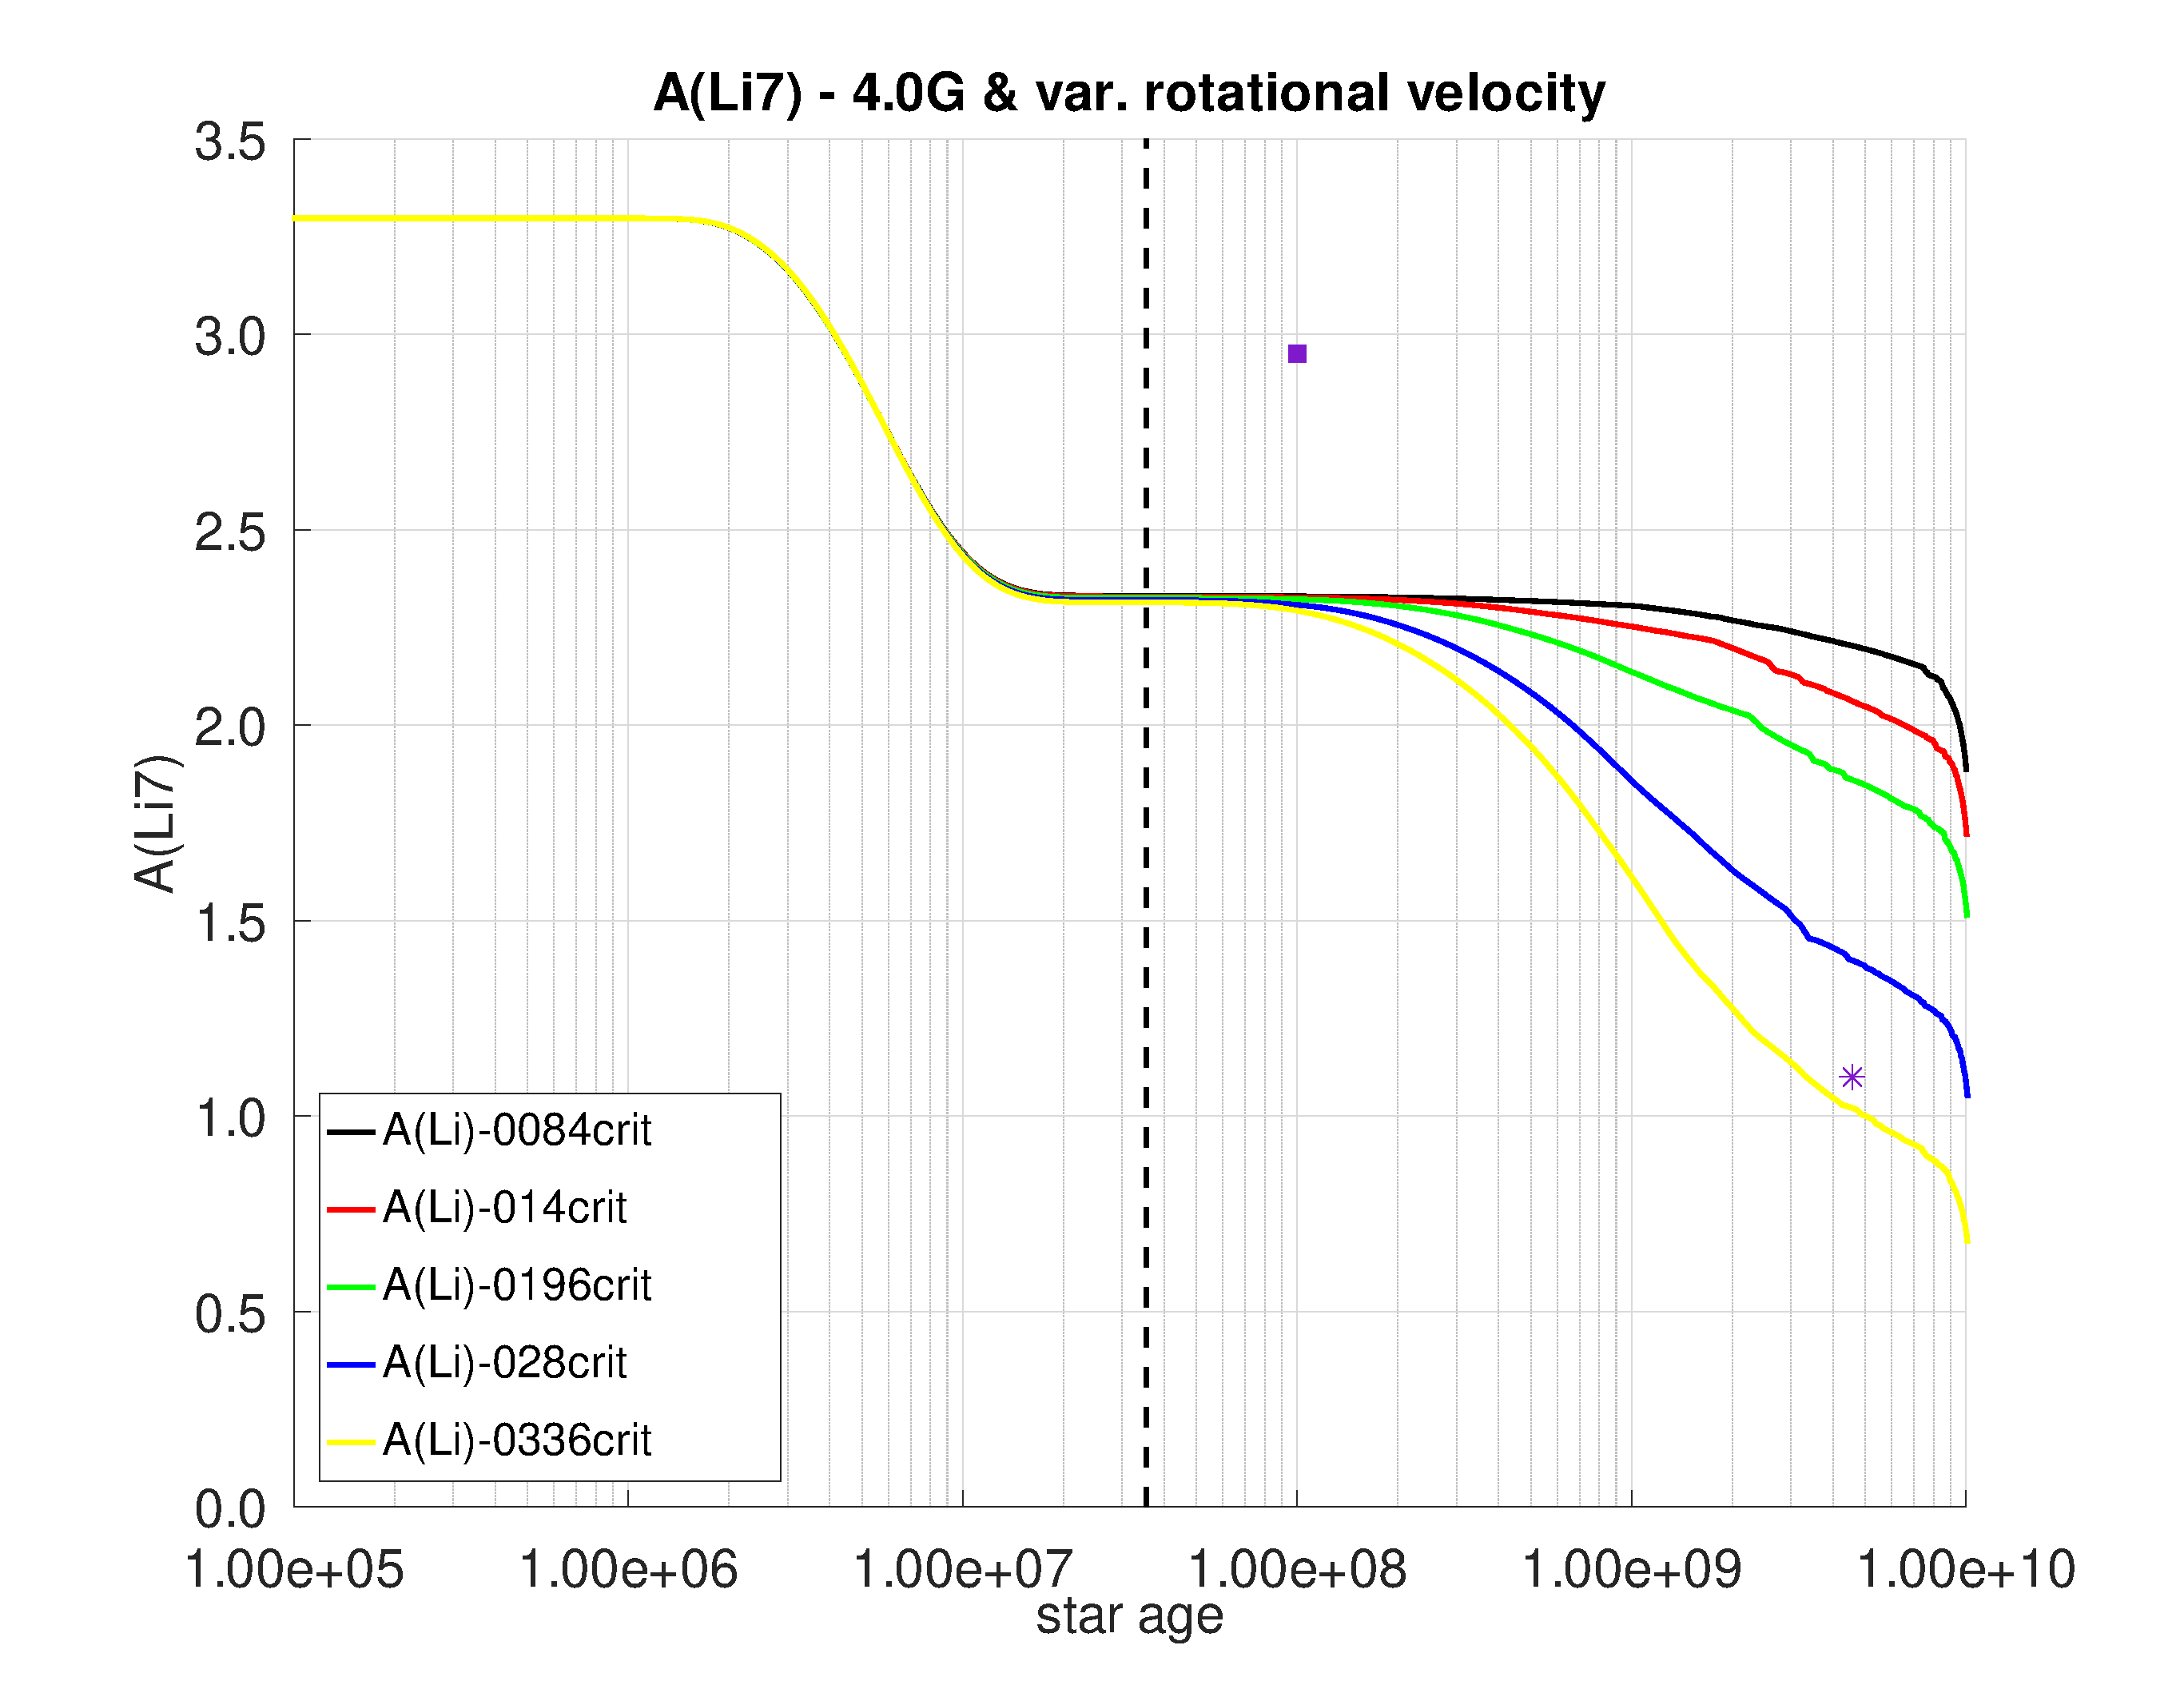
\includegraphics[trim = 35mm 15mm 20mm 15mm, clip,width=\textwidth]{figures/li_var_vel_4_0g.eps}
    \label{fig:subim4}
    \end{subfigure}
    \begin{subfigure}[h]{0.47\textwidth}
    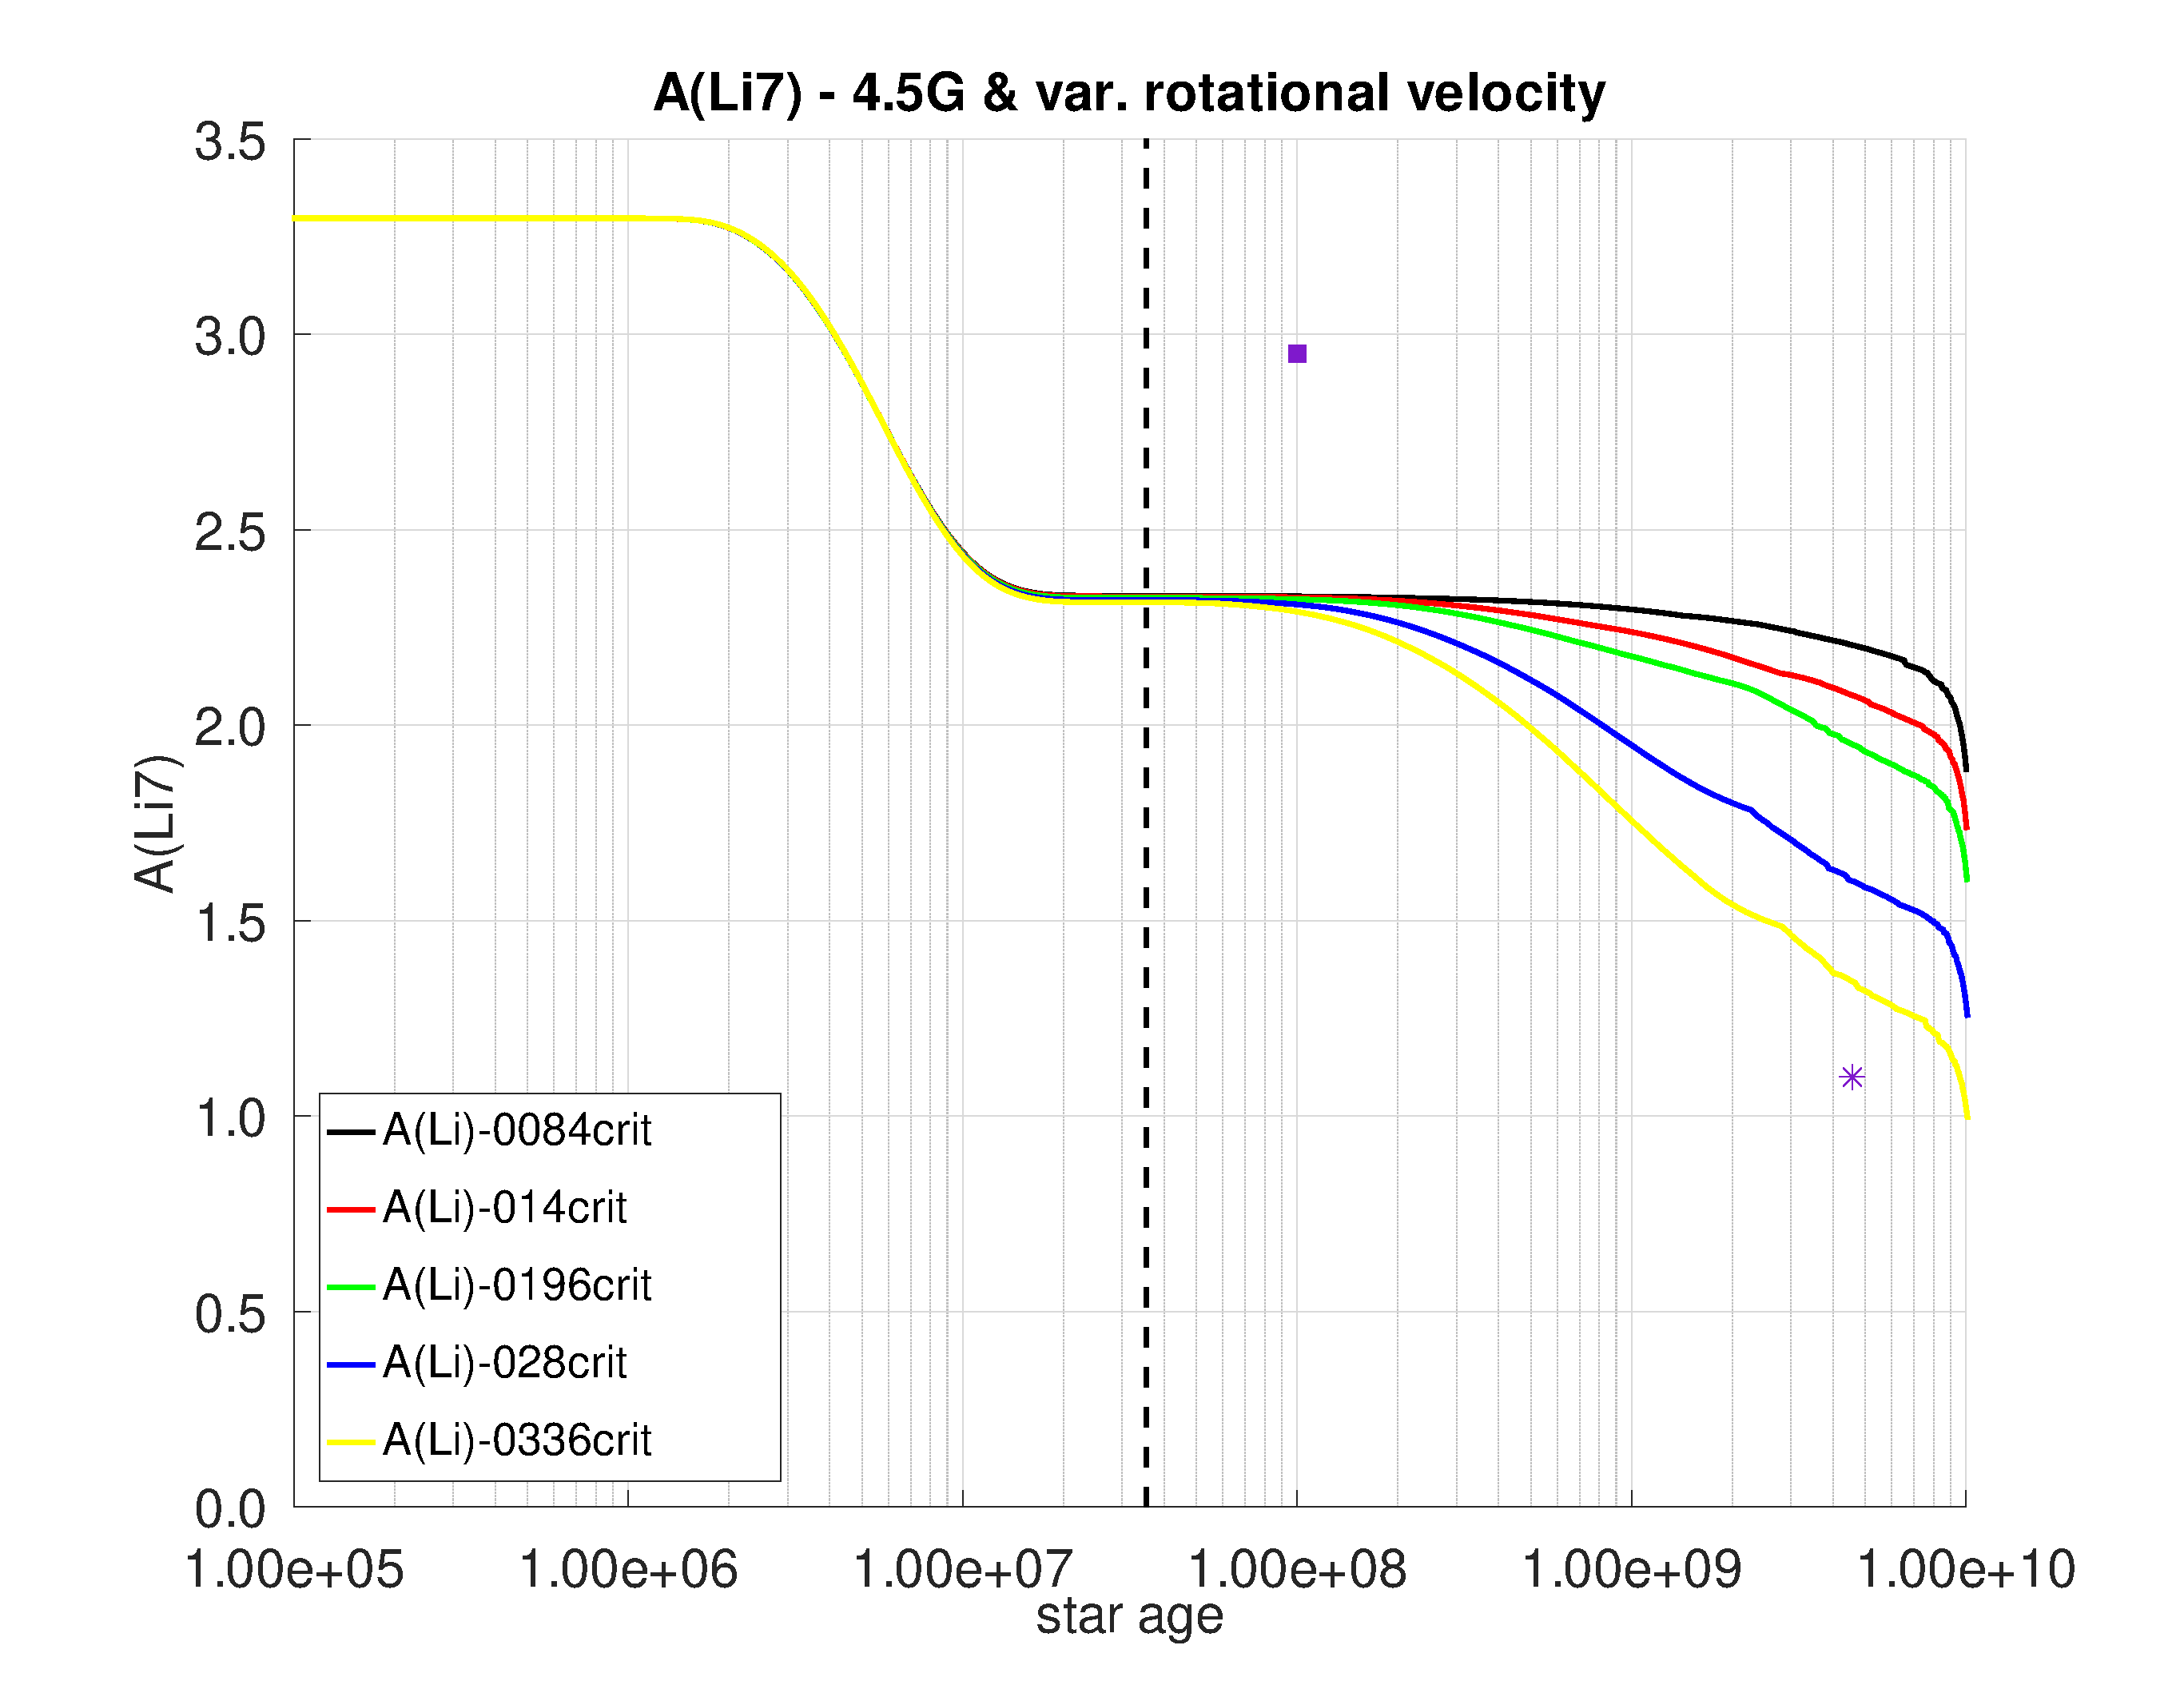
\includegraphics[trim = 35mm 15mm 20mm 15mm, clip,width=\textwidth]{figures/li_var_vel_4_5g.eps}
    \label{fig:subim5}
    \end{subfigure}
    \begin{subfigure}[h]{0.47\textwidth}
    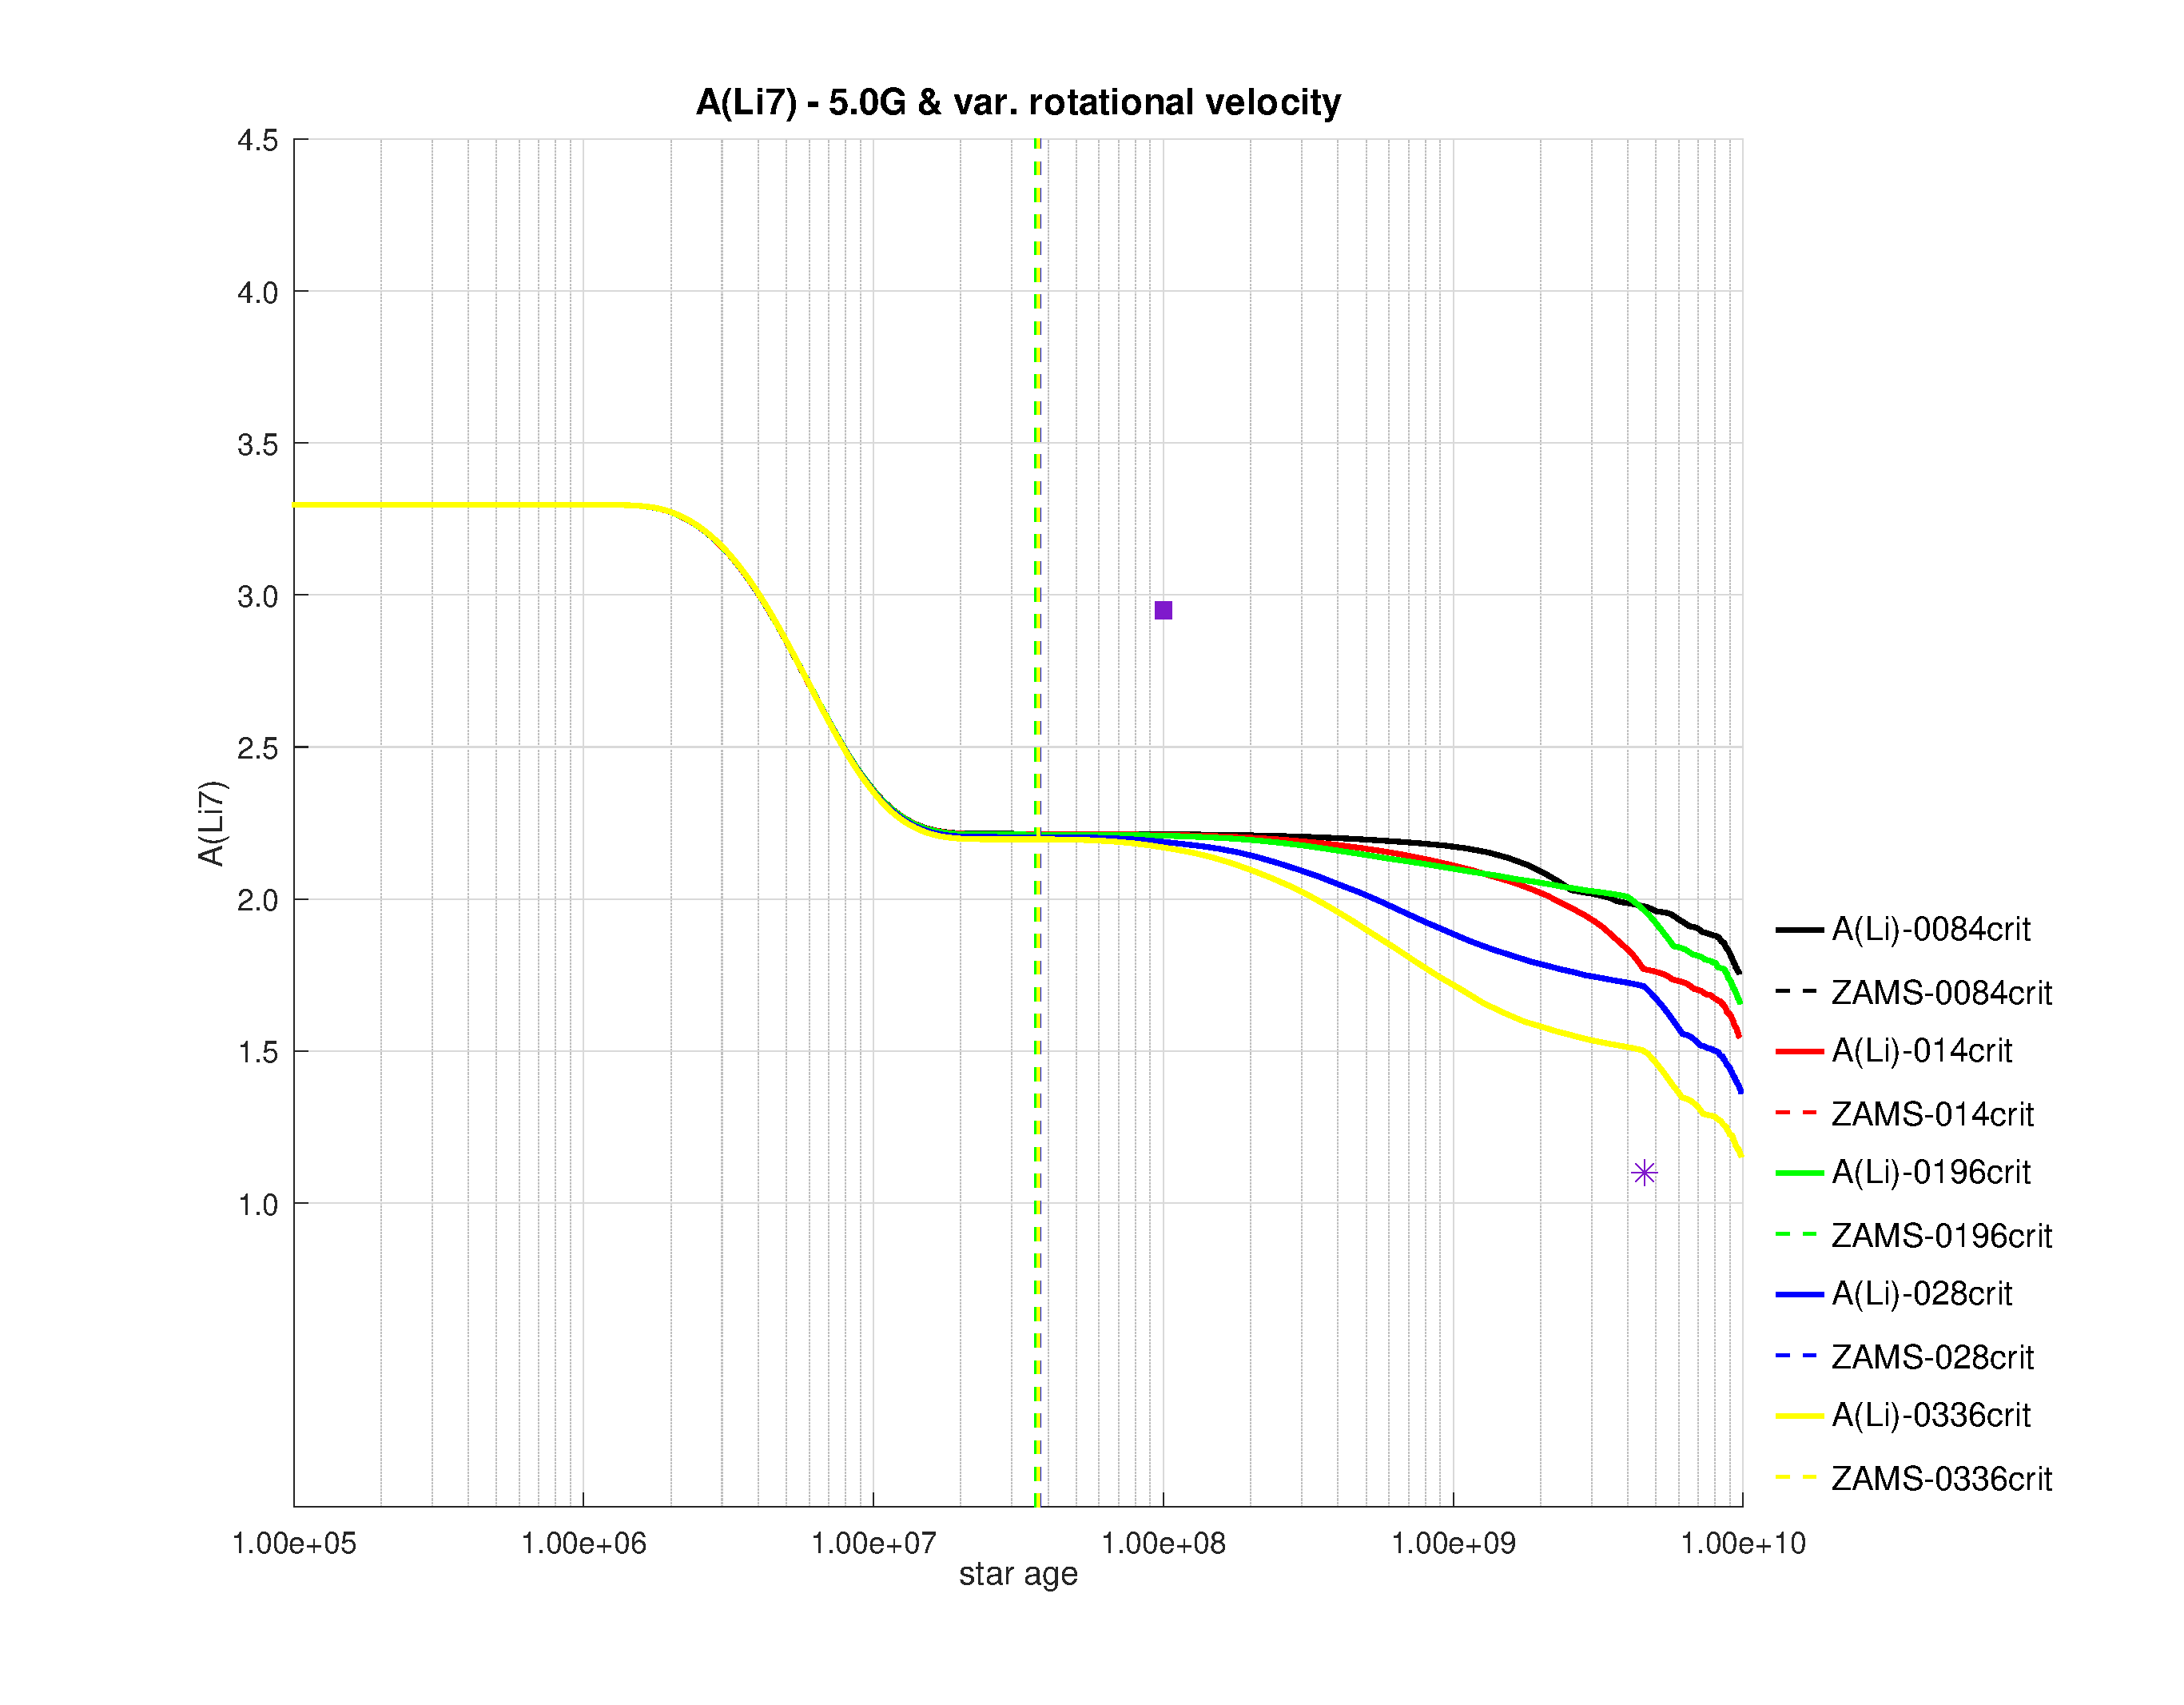
\includegraphics[trim = 35mm 15mm 20mm 15mm, clip,width=\textwidth]{figures/li_var_vel_5_0g.eps}
    \label{fig:subim6}
    \end{subfigure}
\caption{Grid showing the evolution of surface \isotope[7]{Li} abundance relative to \isotope[1]{H}, as a function of time for several 1 $\msun$ models. Each figure shows a set of models in which the magnetic field with intensity has been fixed and $\oomegac$ varies between 0.0084 and 0.0336, respectively. The purple star and square are surface Li abundance for the present-day Sun \citep{Asplund2009} and the Pleiades cluster \citep{Sestito2005} respectively. The dashed lines make reference to the ZAMS.}
\label{fig:grid_li_var_vel}
\end{figure*}
\par


\begin{figure*}
    \centering
    \begin{subfigure}[h]{0.47\textwidth}
    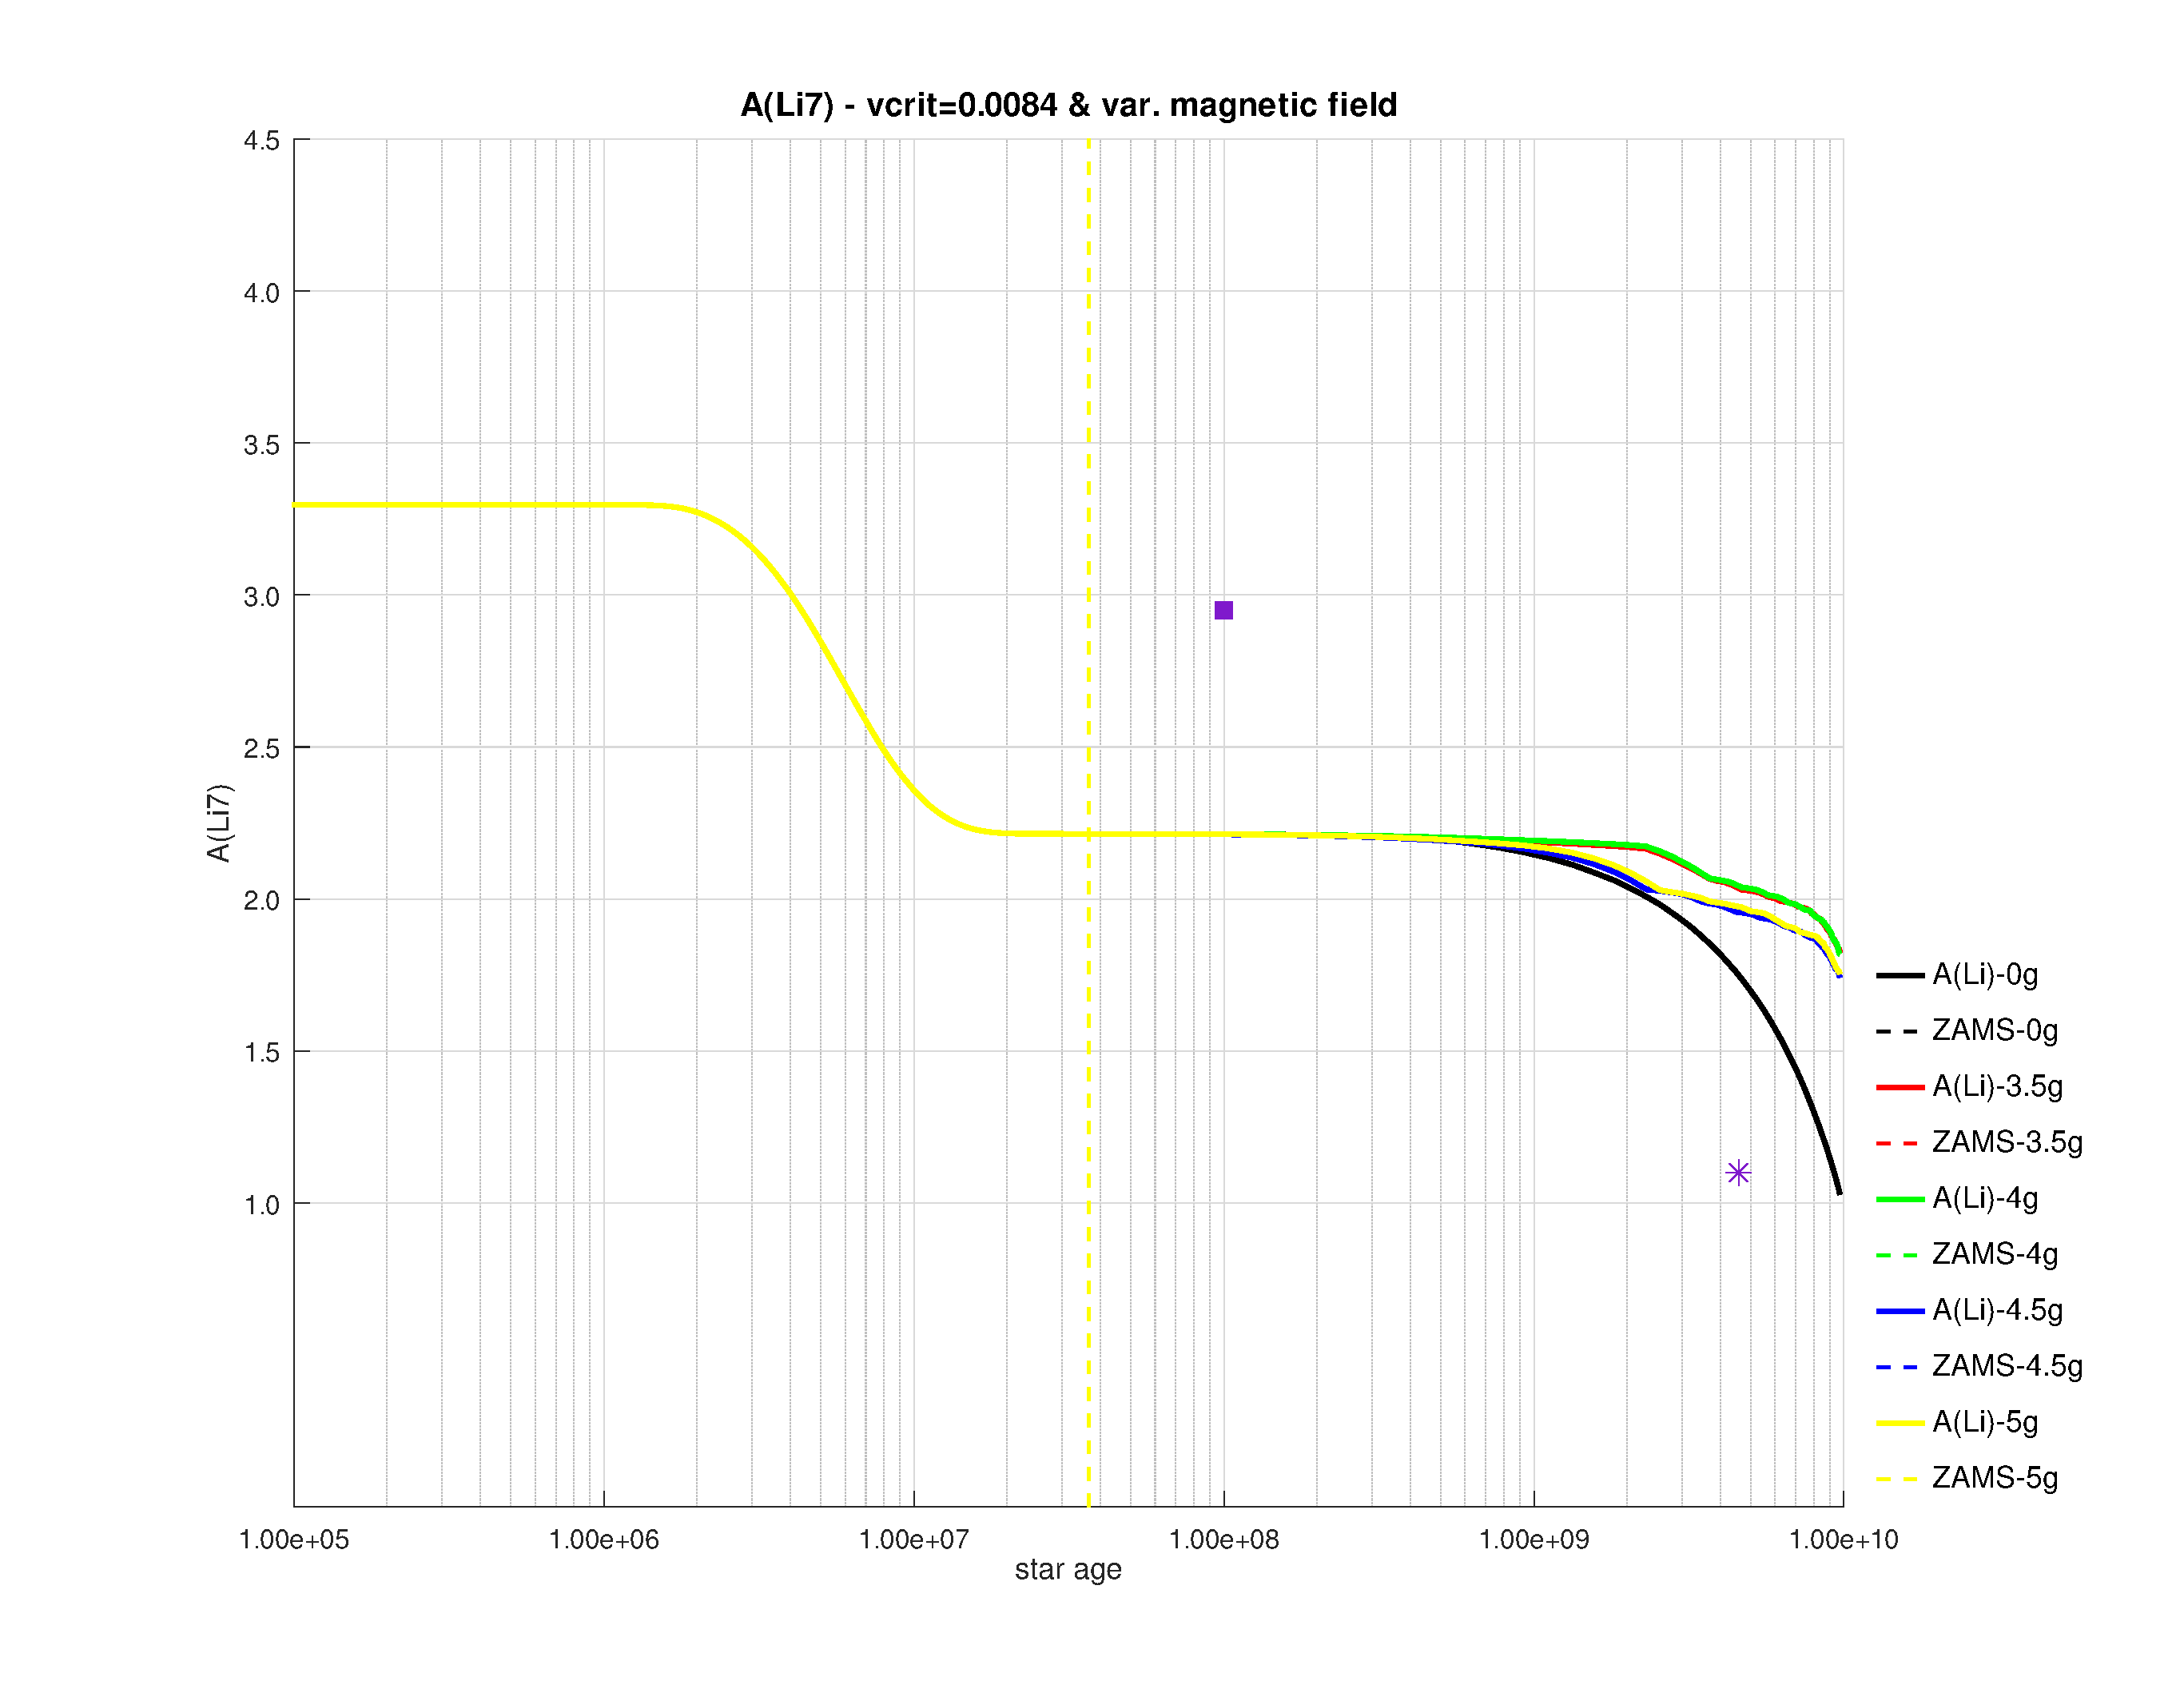
\includegraphics[trim = 35mm 15mm 15mm 15mm, clip,width=\textwidth]{figures/li_vc_0084_var_g.eps}
    \label{fig:subim21}
    \end{subfigure}
    \begin{subfigure}[h]{0.47\textwidth}
    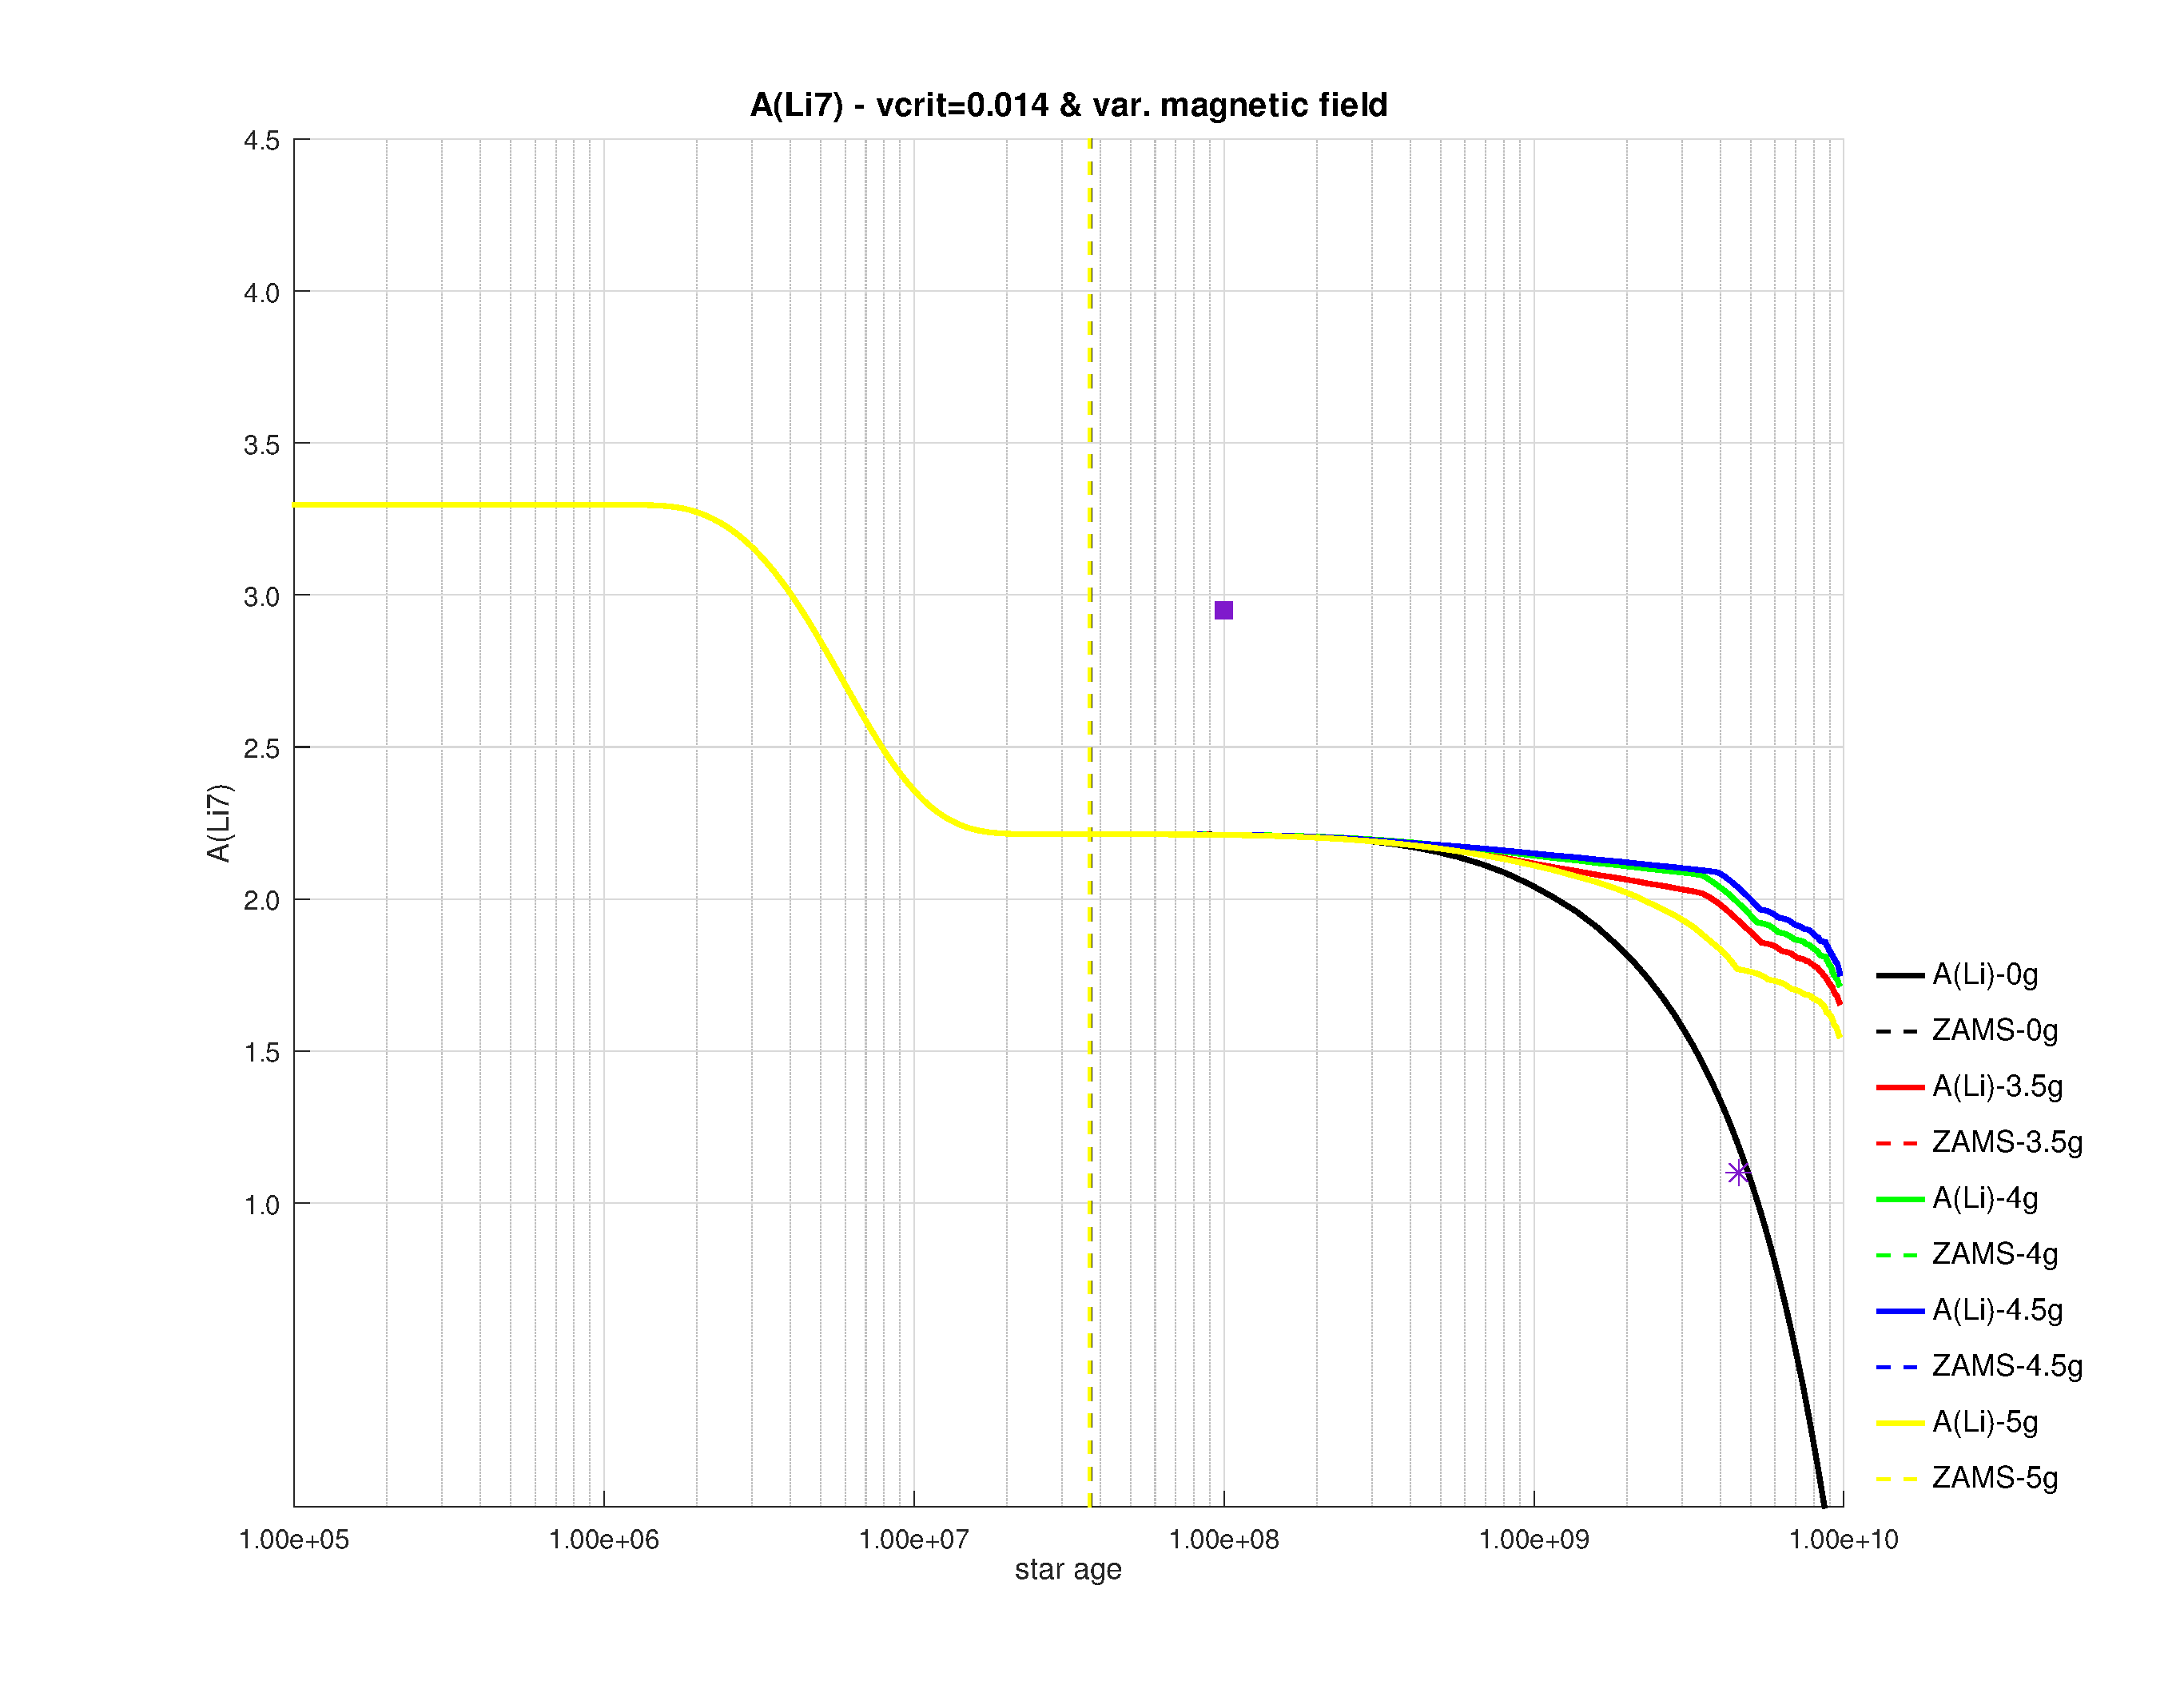
\includegraphics[trim = 35mm 15mm 15mm 15mm, clip,width=\textwidth]{figures/li_vc_014_var_g.eps}
    \label{fig:subim22}
    \end{subfigure}
    \begin{subfigure}[h]{0.47\textwidth}
    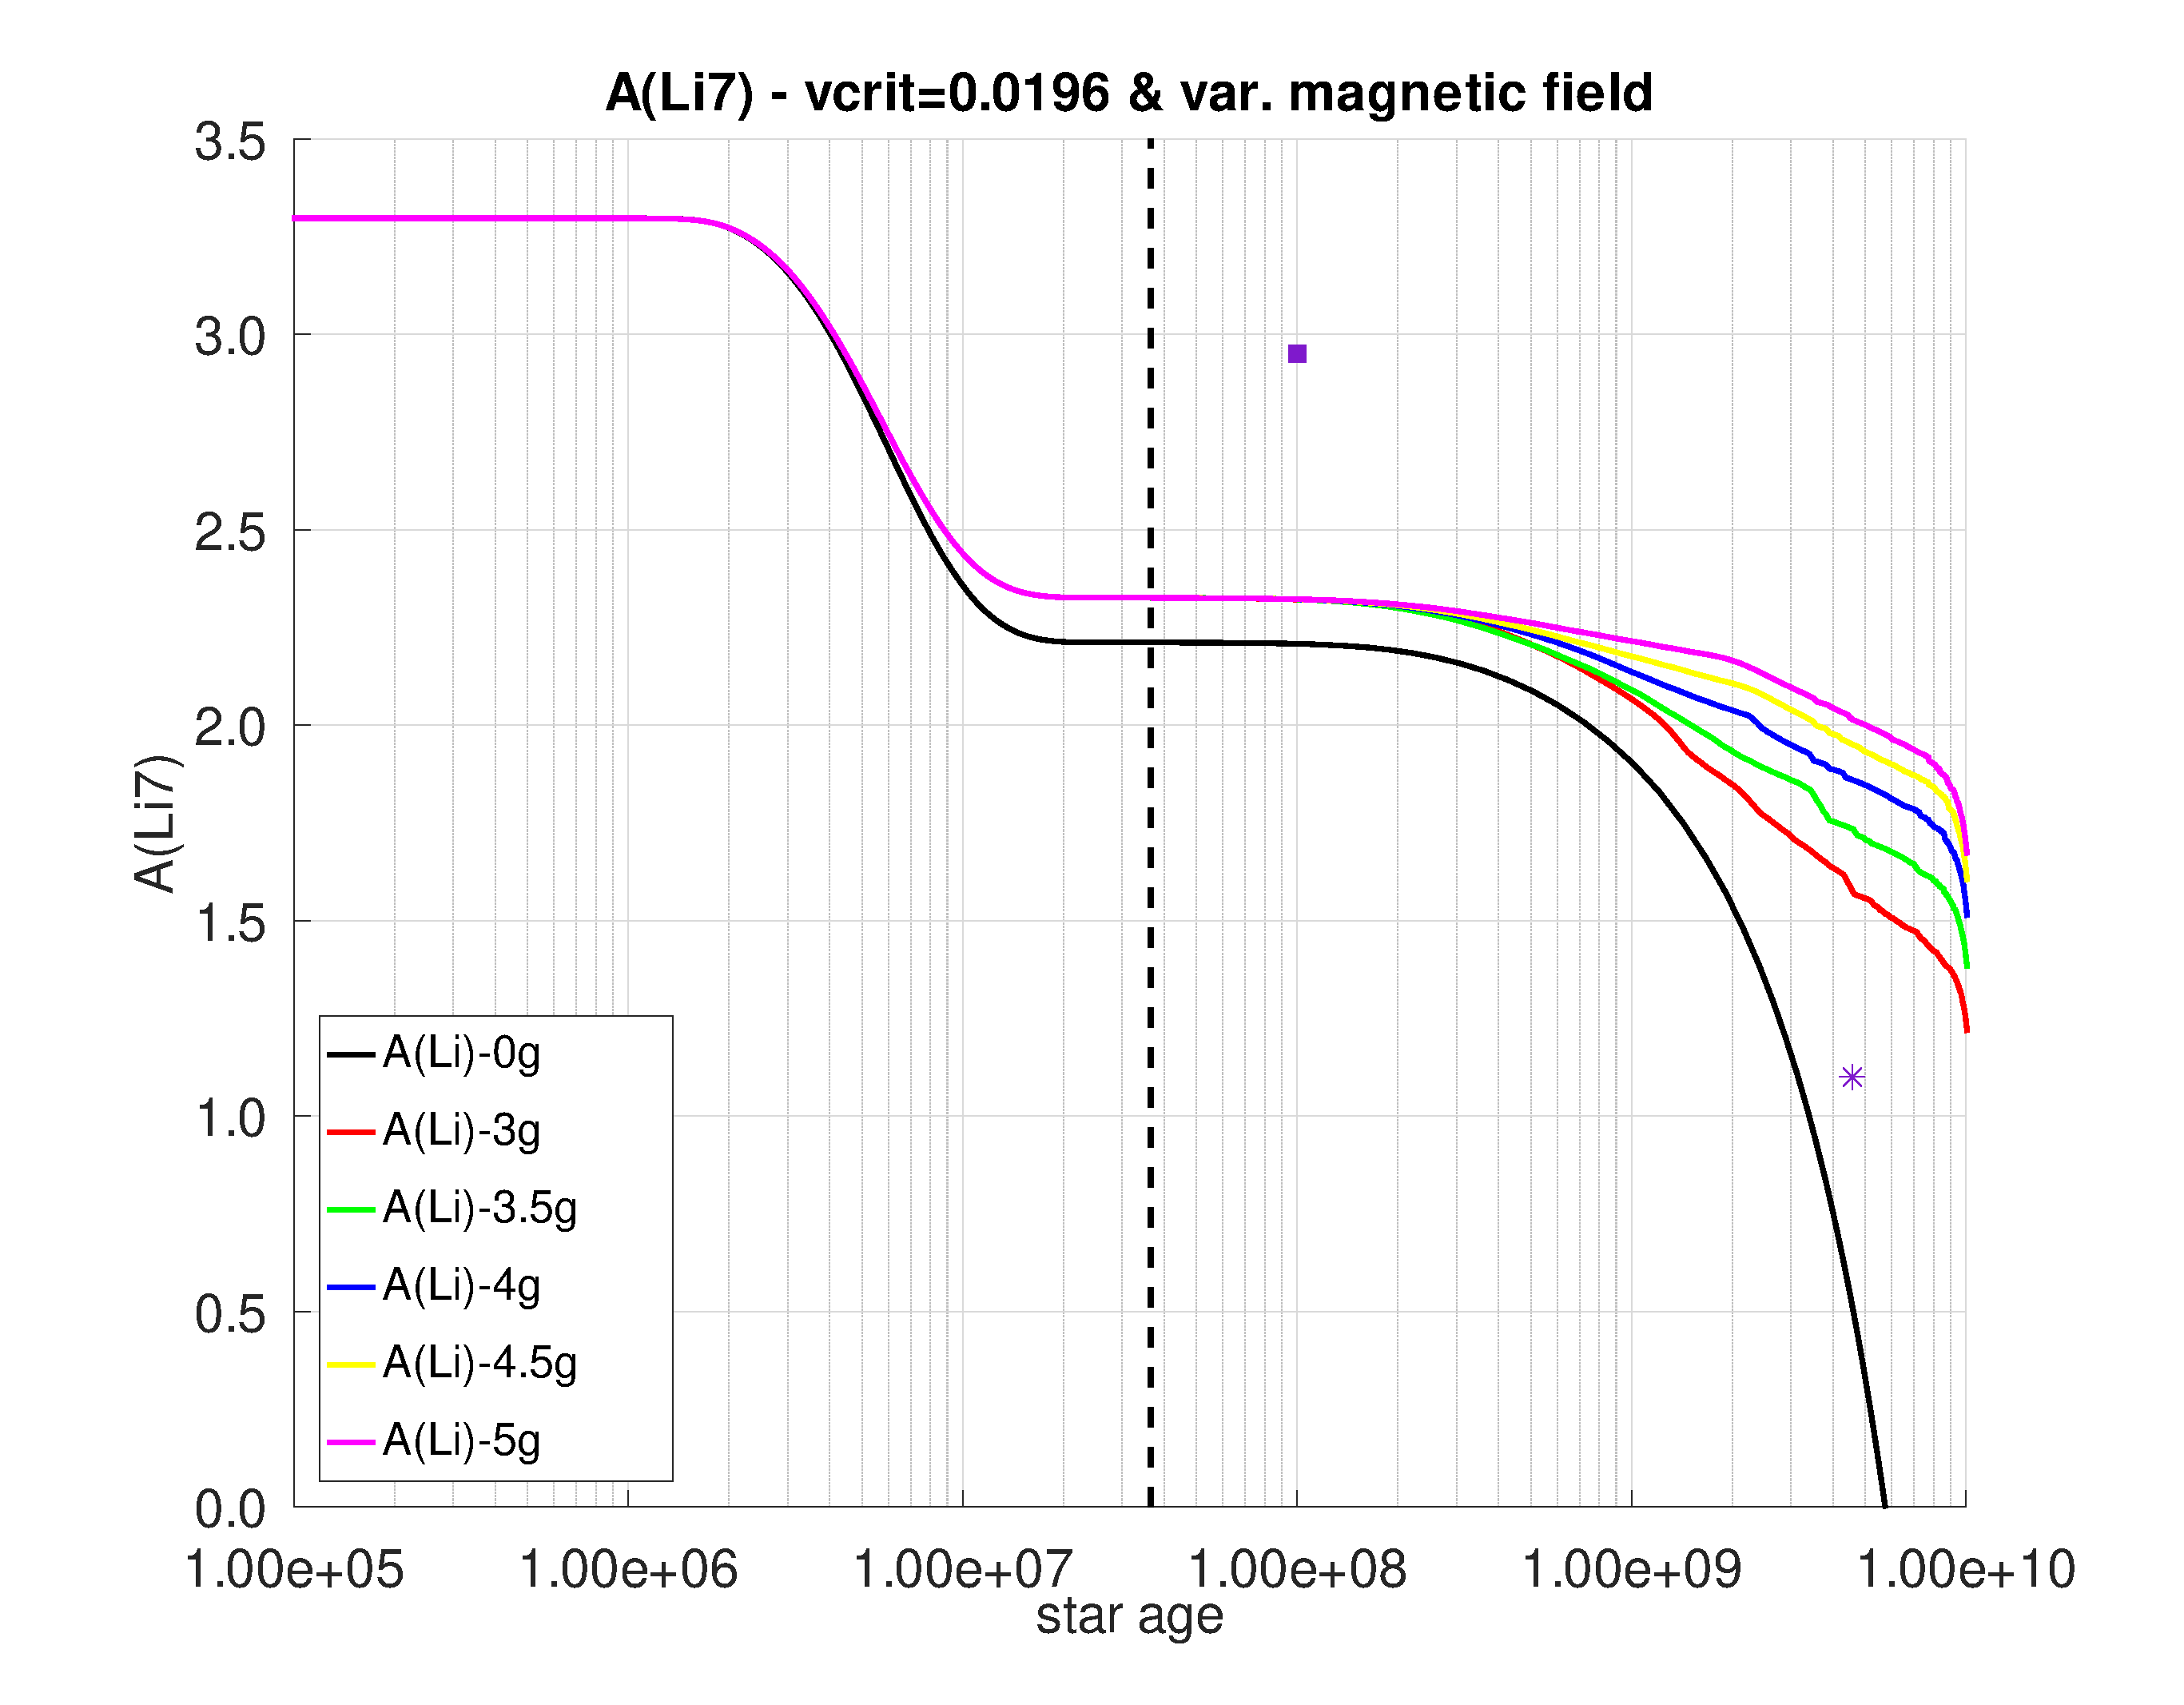
\includegraphics[trim = 35mm 15mm 15mm 15mm, clip,width=\textwidth]{figures/li_vc_0196_var_g.eps}
    \label{fig:subim23}
    \end{subfigure}
    \begin{subfigure}[h]{0.47\textwidth}
    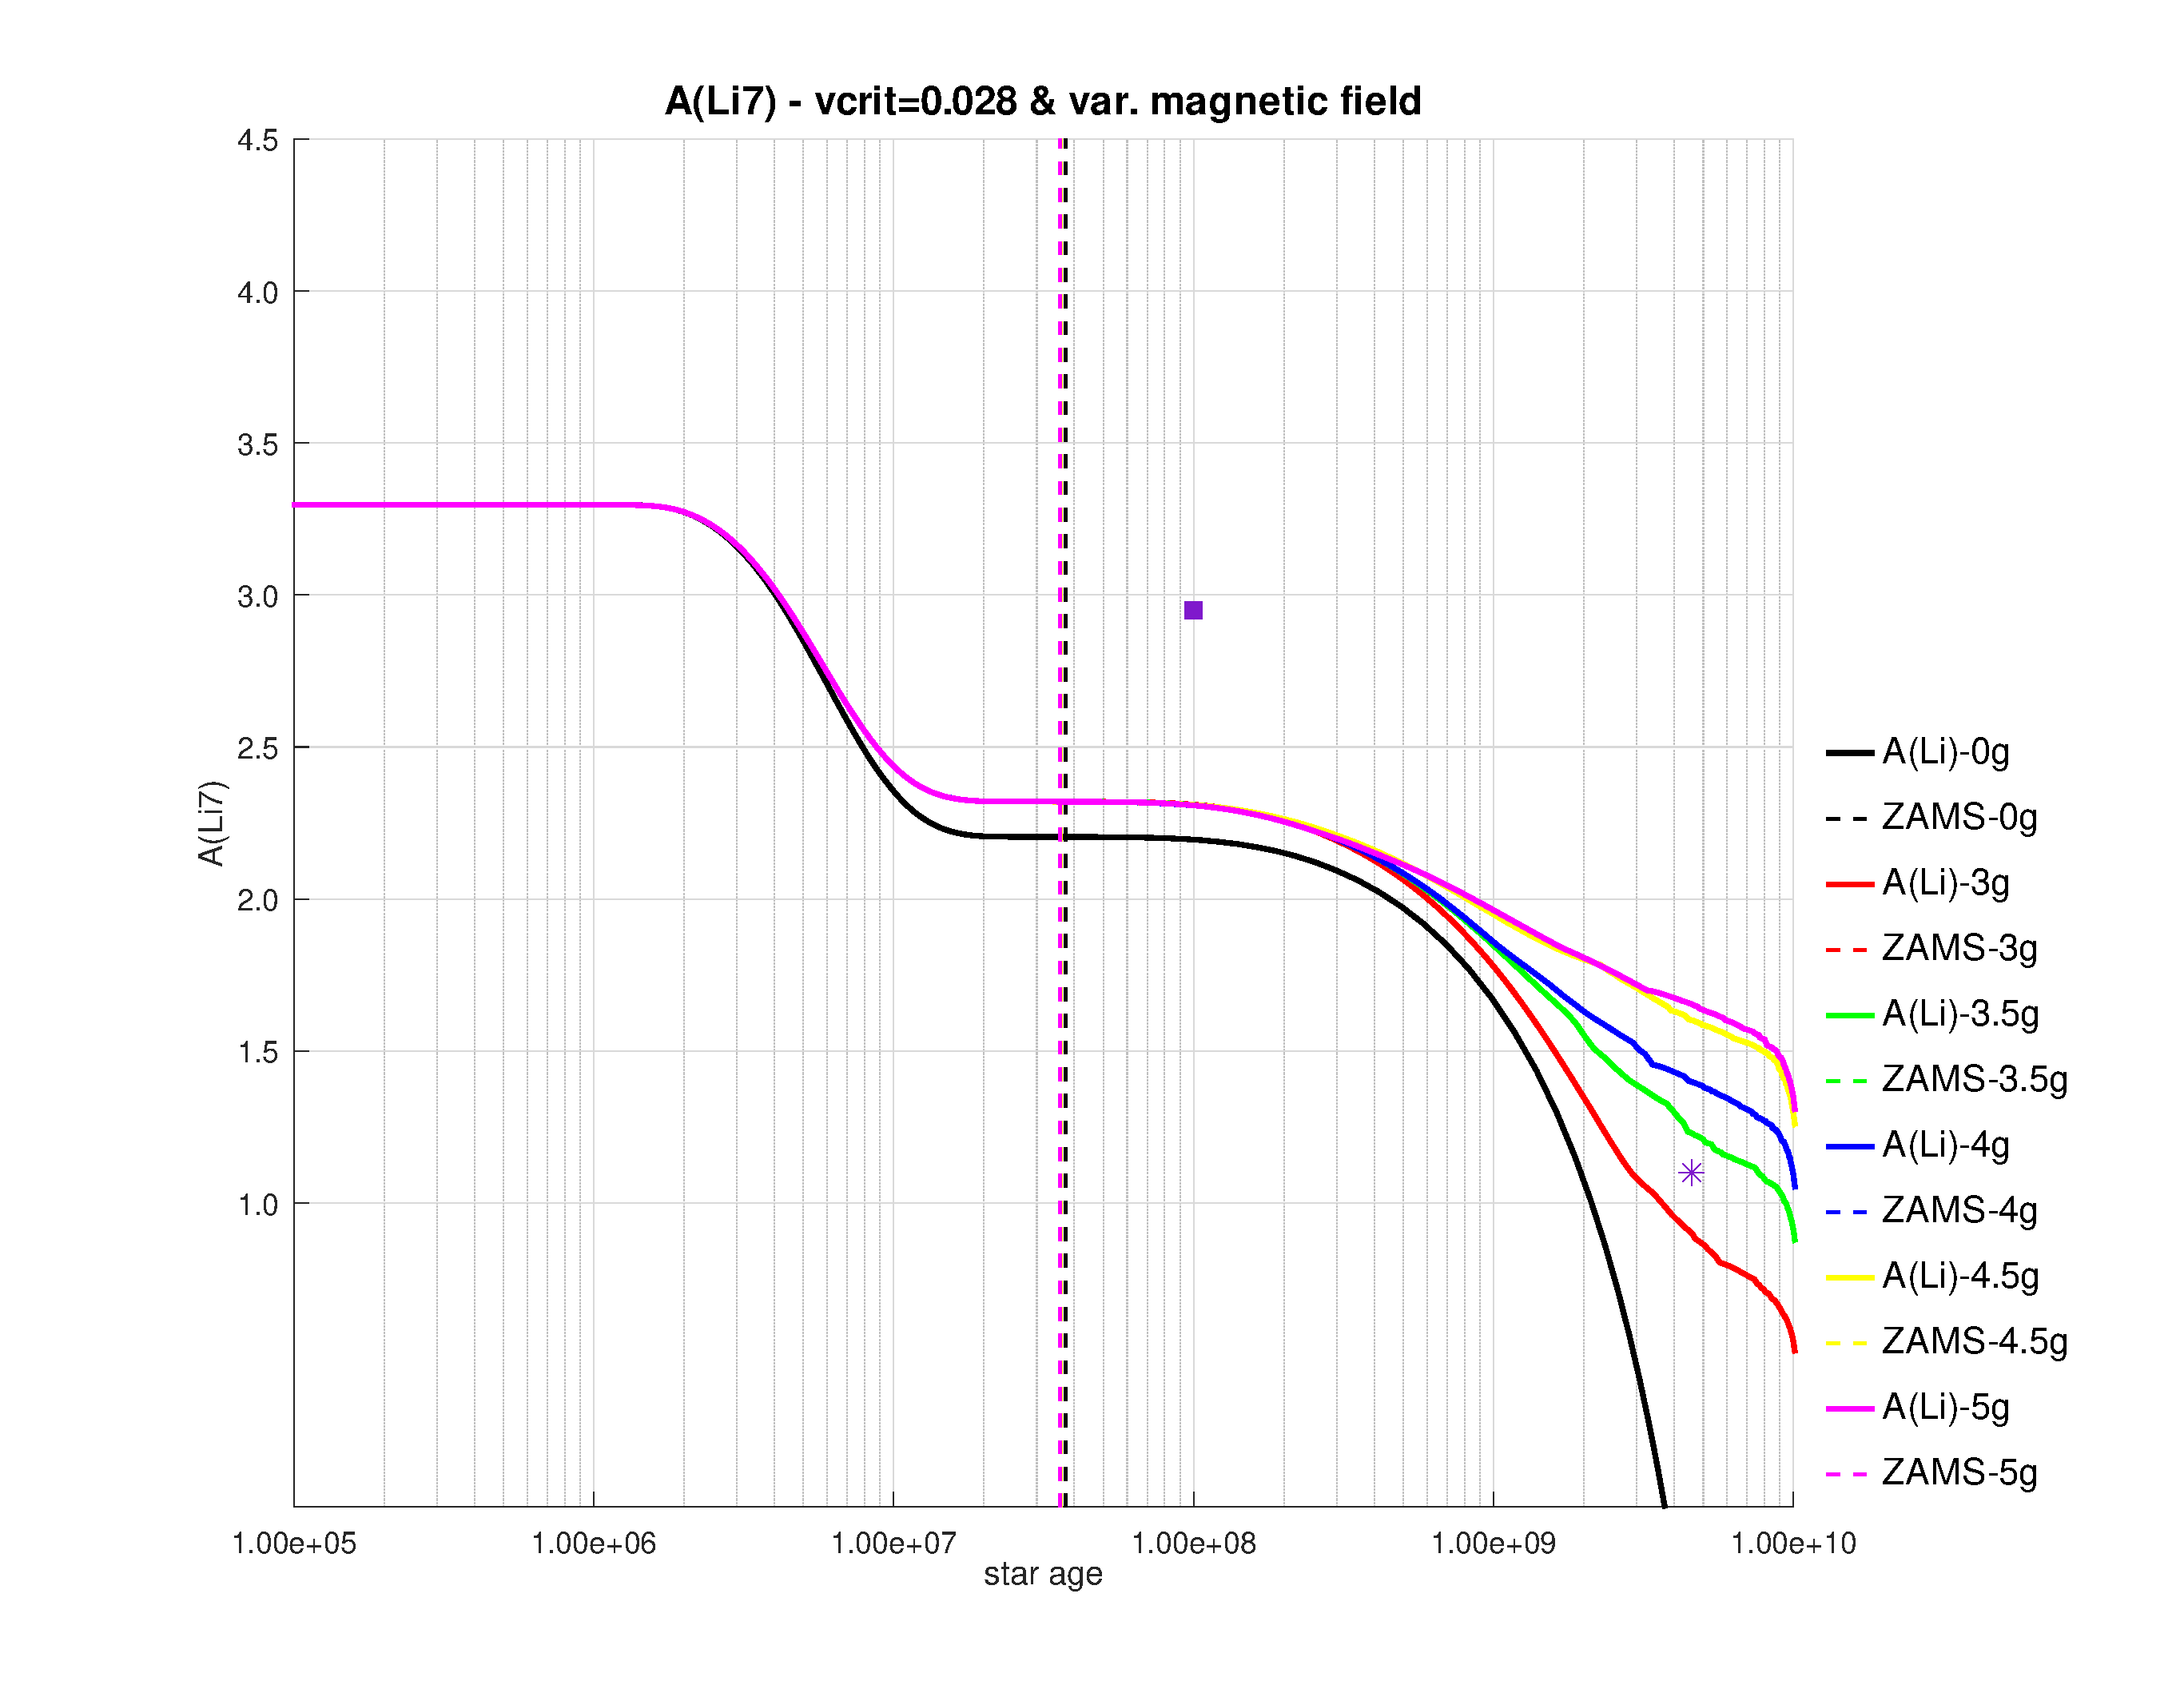
\includegraphics[trim = 35mm 15mm 15mm 15mm, clip,width=\textwidth]{figures/li_vc_028_var_g.eps}
    \label{fig:subim24}
    \end{subfigure}
    \begin{subfigure}[h]{0.47\textwidth}
    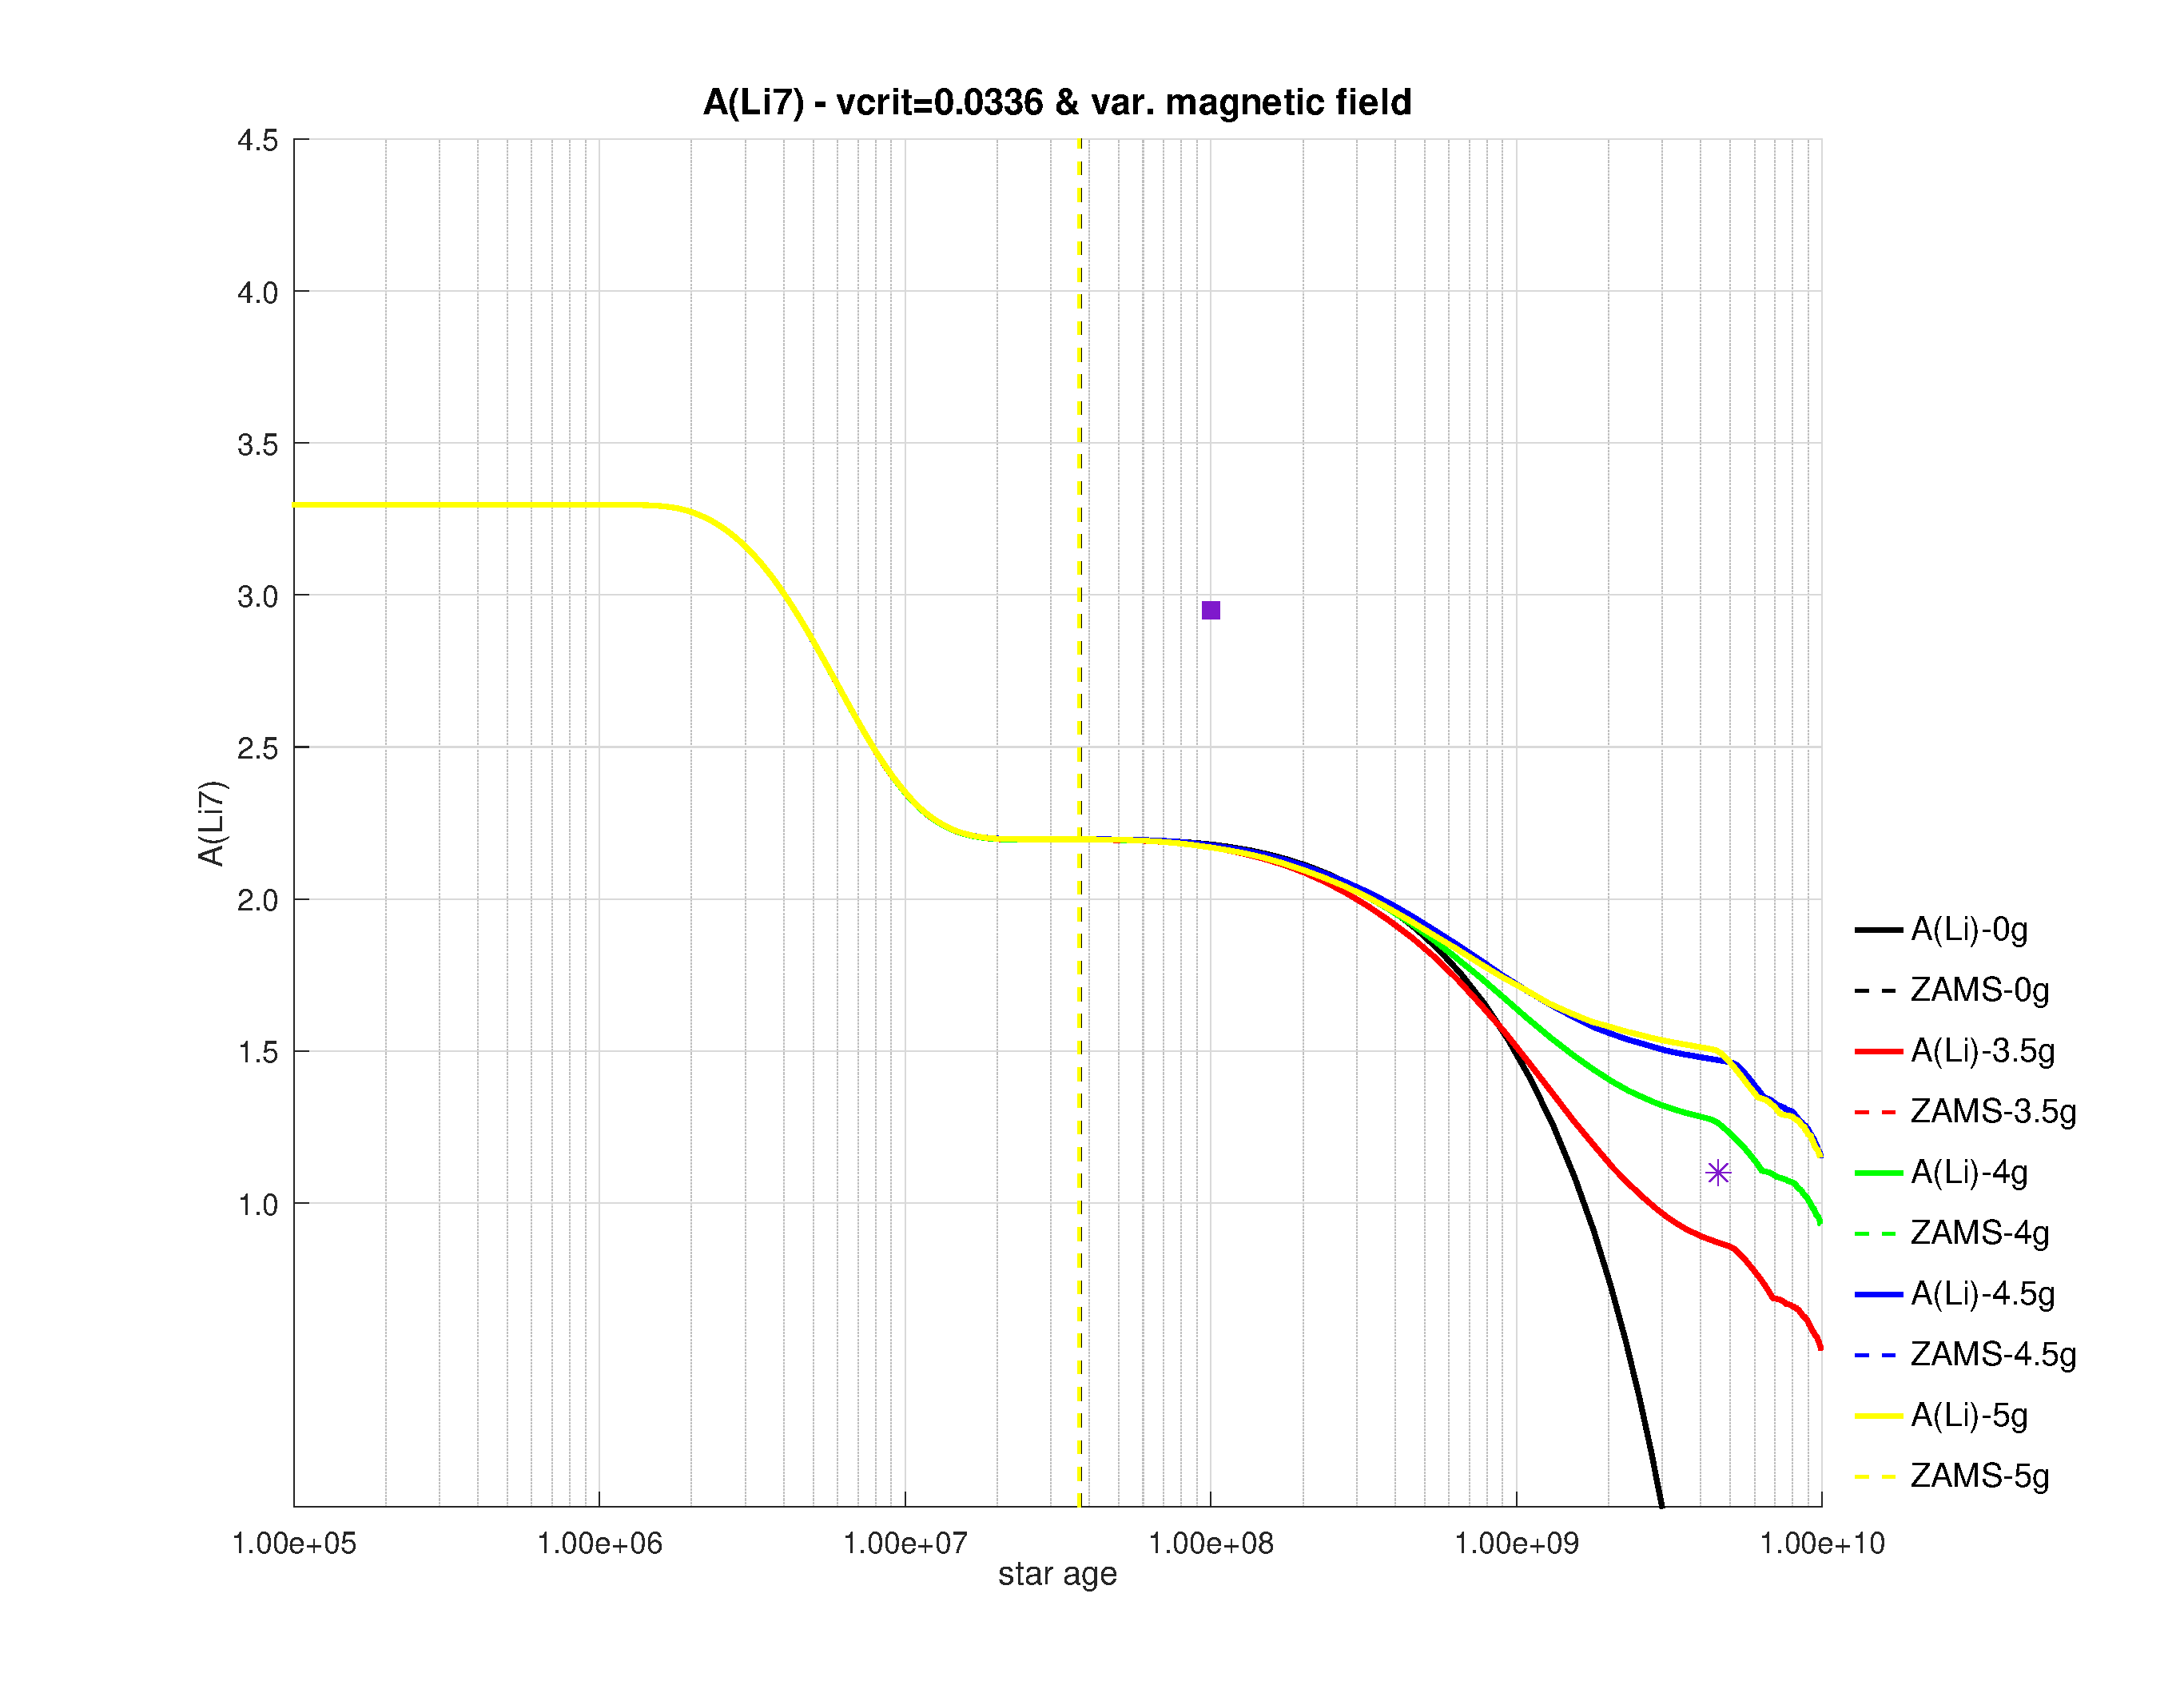
\includegraphics[trim = 35mm 15mm 15mm 15mm, clip,width=\textwidth]{figures/li_vc_0336_var_g.eps}
    \label{fig:subim25}
    \end{subfigure}
    \begin{subfigure}[h]{0.47\textwidth}
    
\includegraphics[width=\textwidth]{figures/blank.eps}
    \label{fig:subim26}
    \end{subfigure}
\caption{Grid showing the evolution of surface \isotope[7]{Li} abundance relative to \isotope[1]{H}, as a function of time for several 1 $\msun$ models. Each figure shows a set of models in which $\oomegac$ has been fixed and the magnetic field with intensity varies between $0.0\,\Gauss$ and $5.0\,\Gauss$, respectively. The purple star and square are surface Li abundance for the present-day Sun \citep{Asplund2009} and the Pleiades cluster \citep{Sestito2005} respectively. The dashed lines make reference to the ZAMS.}
\label{fig:grid_li_var_g}
\end{figure*}

\begin{figure*}
    \centering
    \begin{subfigure}[h]{0.47\textwidth}
    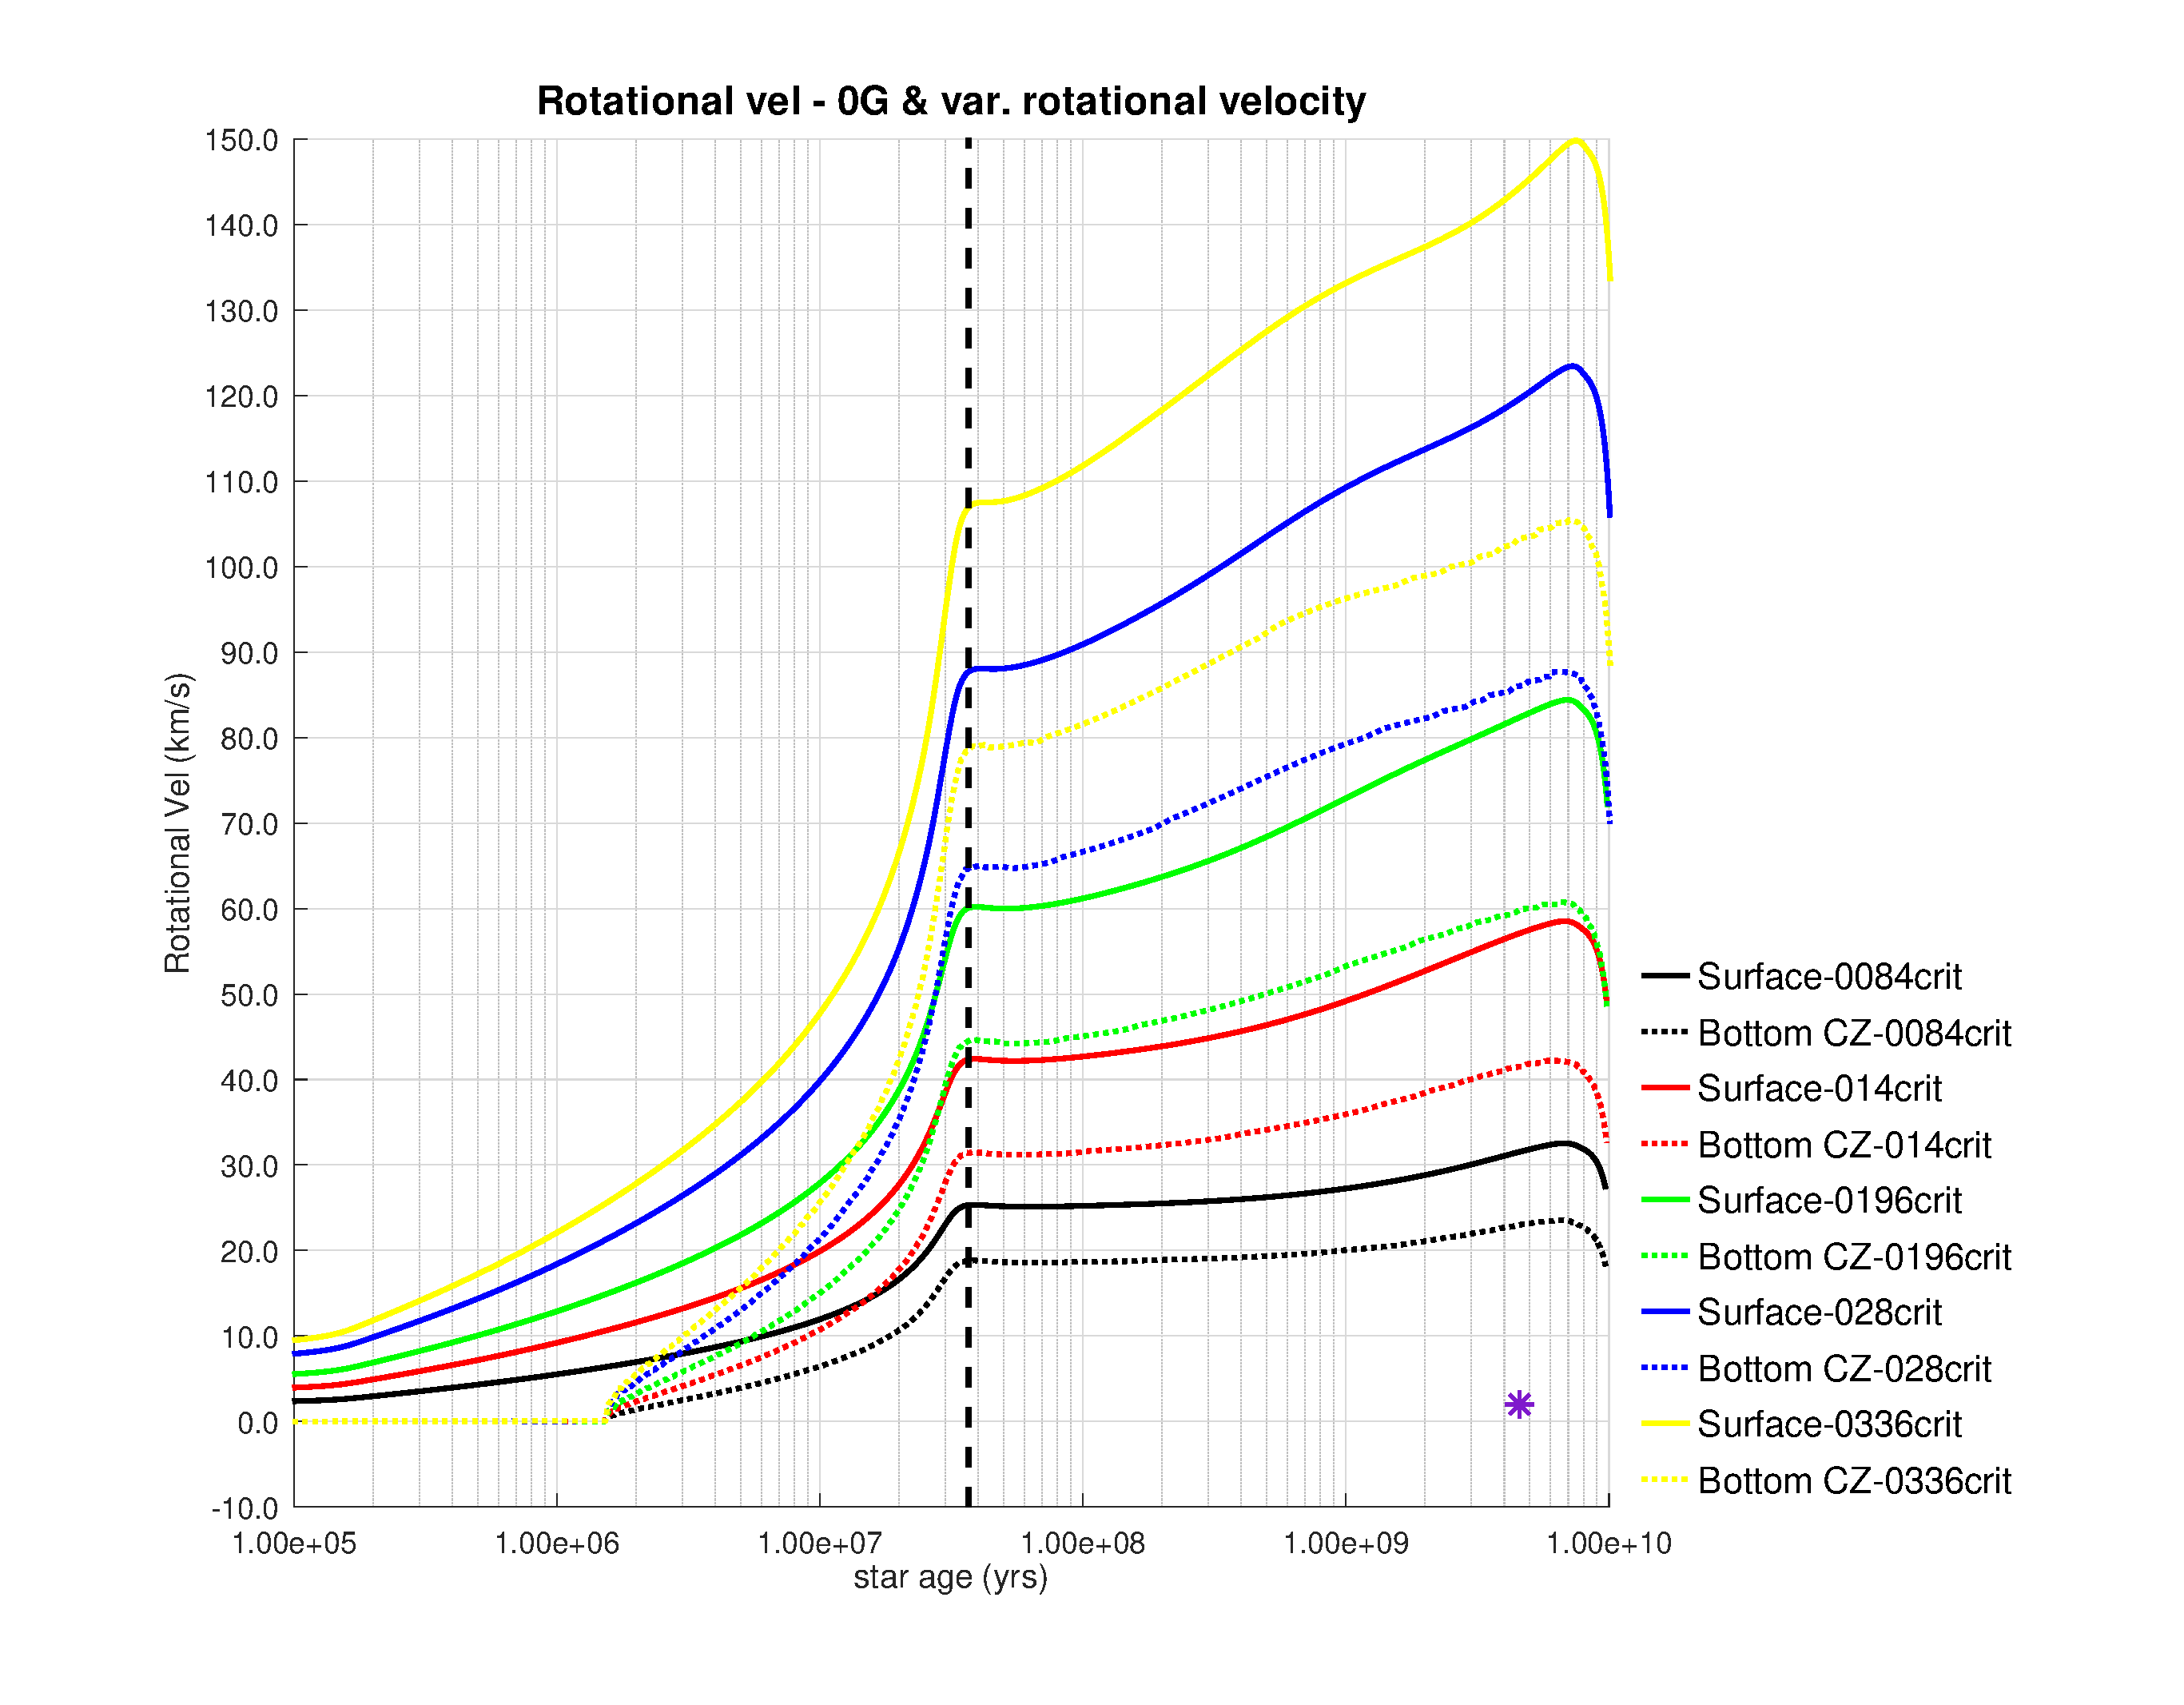
\includegraphics[trim = 30mm 15mm 20mm 15mm, clip,width=\textwidth]{figures/rot_vel_var_vel_0_0g.eps}
    \label{fig:subim41}
    \end{subfigure}
    \begin{subfigure}[h]{0.47\textwidth}
    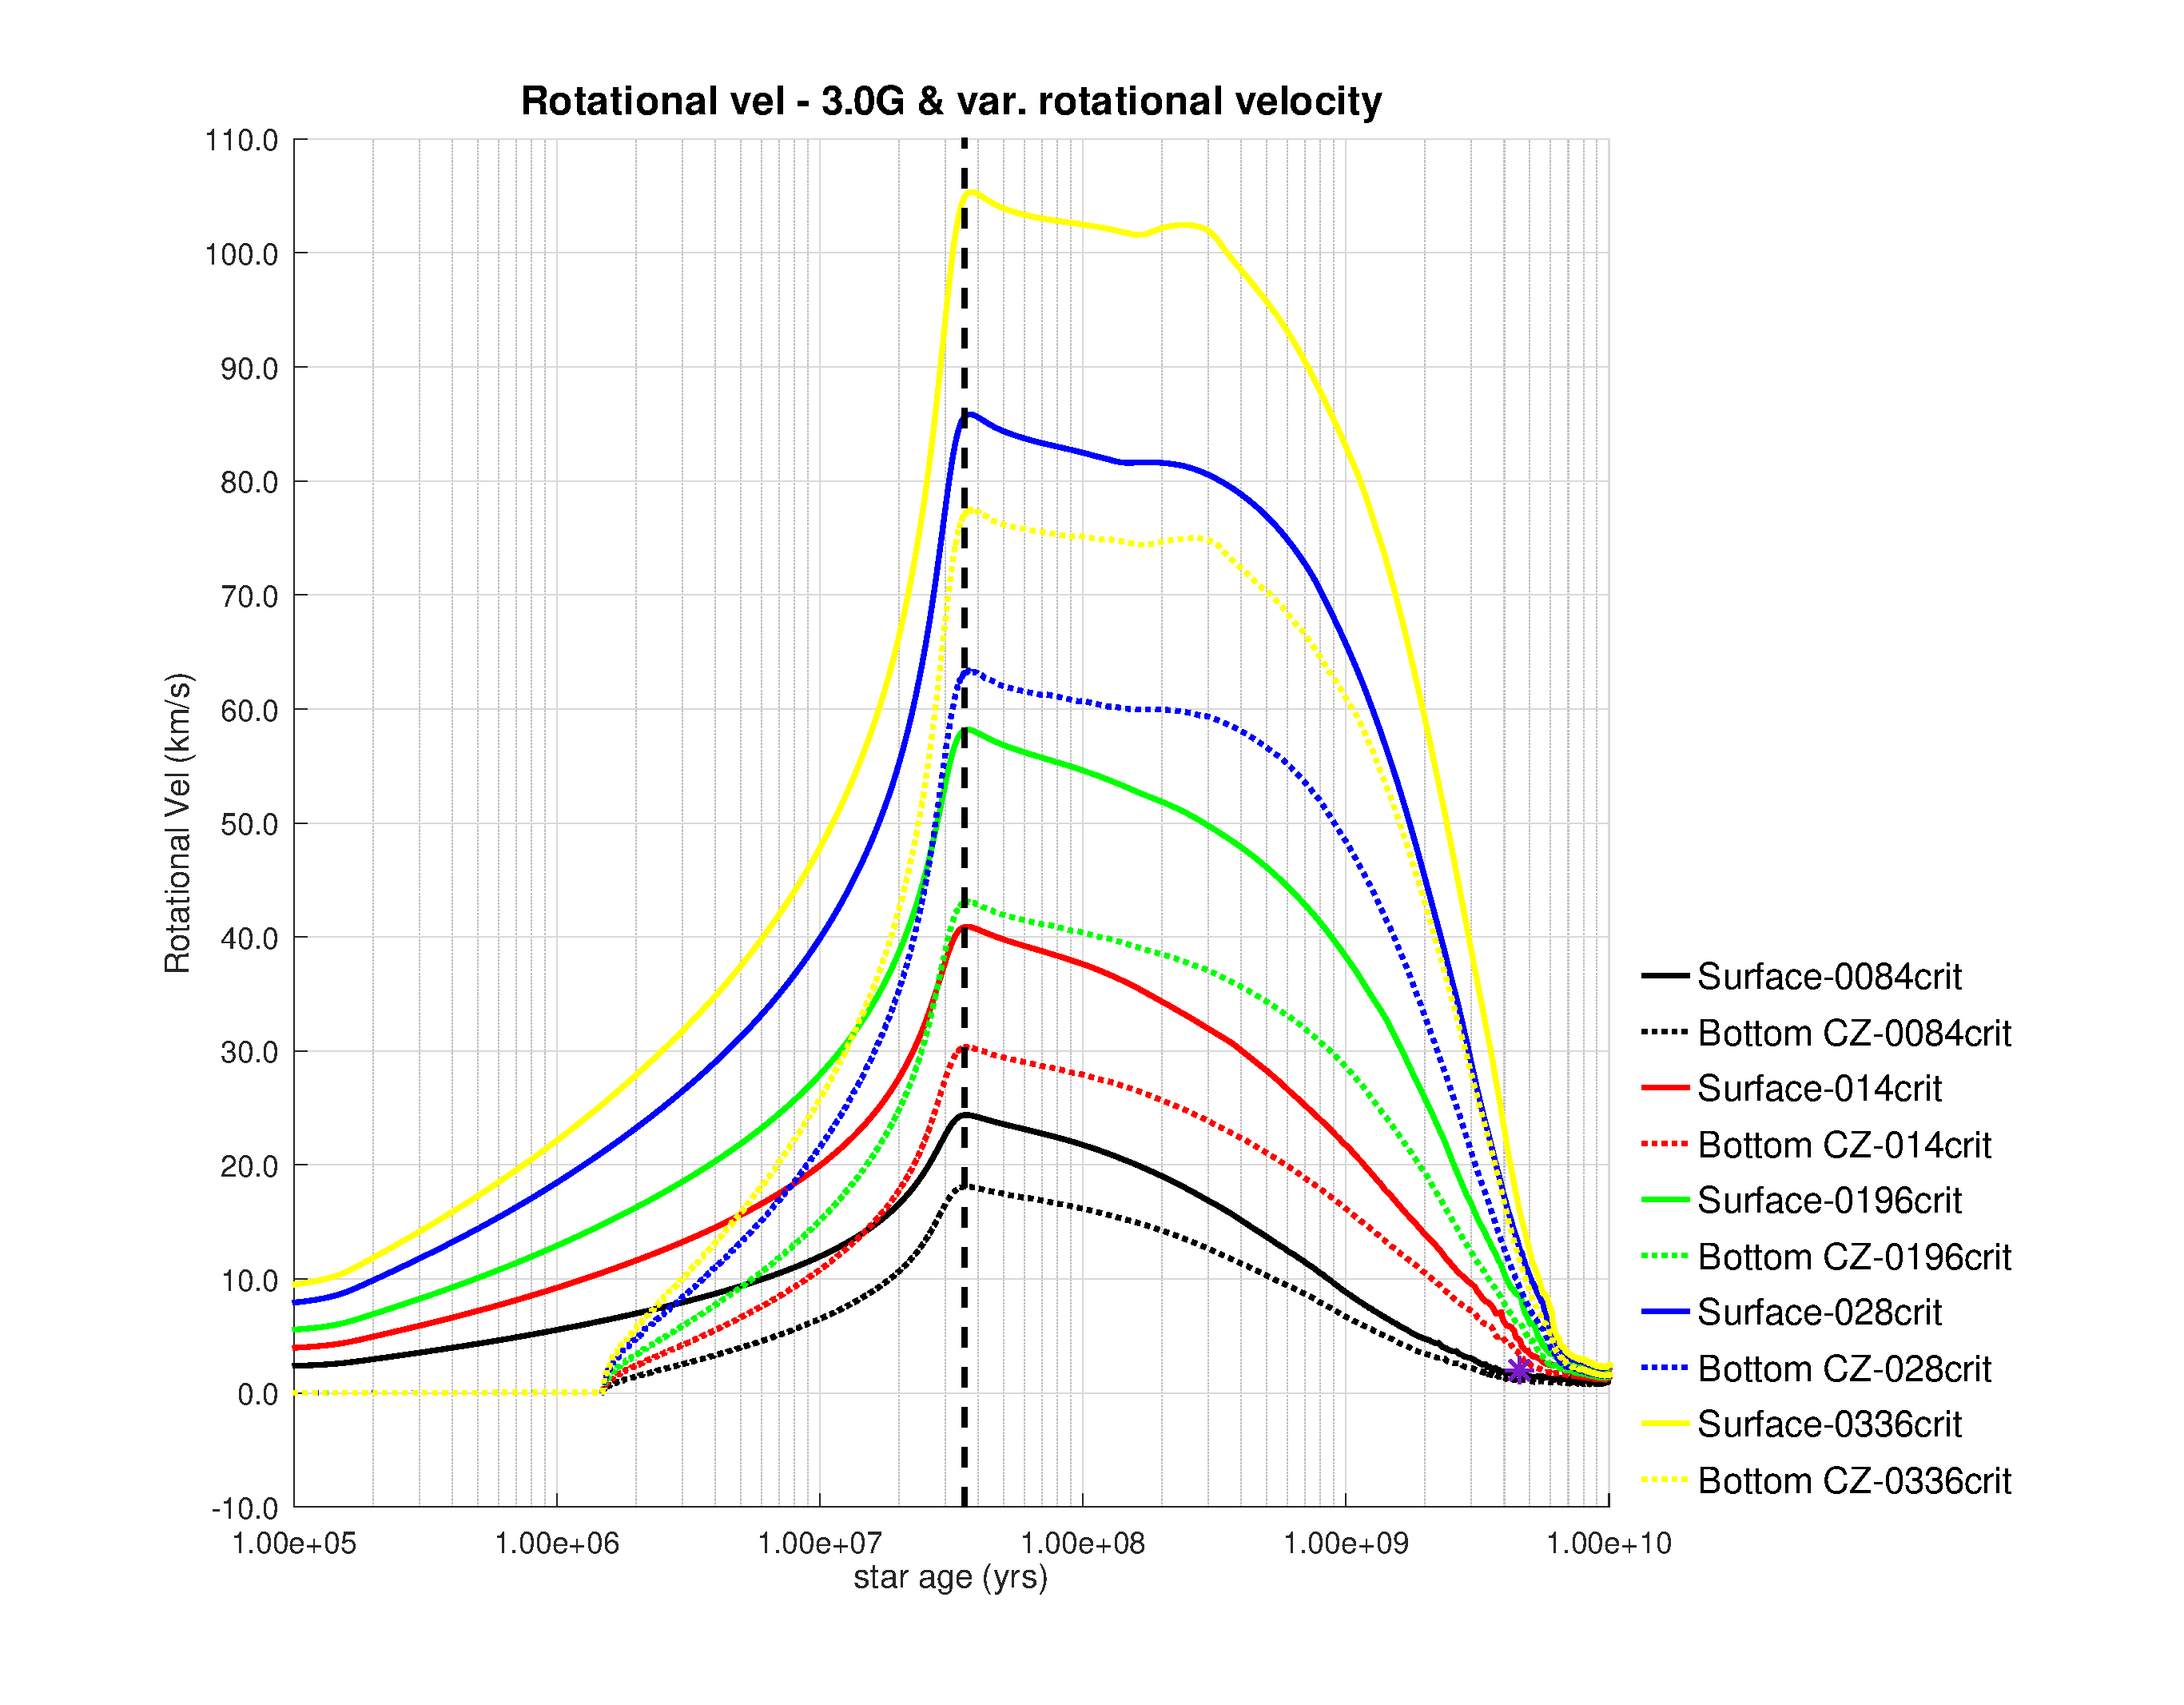
\includegraphics[trim = 30mm 15mm 20mm 15mm, clip,width=\textwidth]{figures/rot_vel_var_vel_3_0g.eps}
    \label{fig:subim42}
    \end{subfigure}
    \begin{subfigure}[h]{0.47\textwidth}
    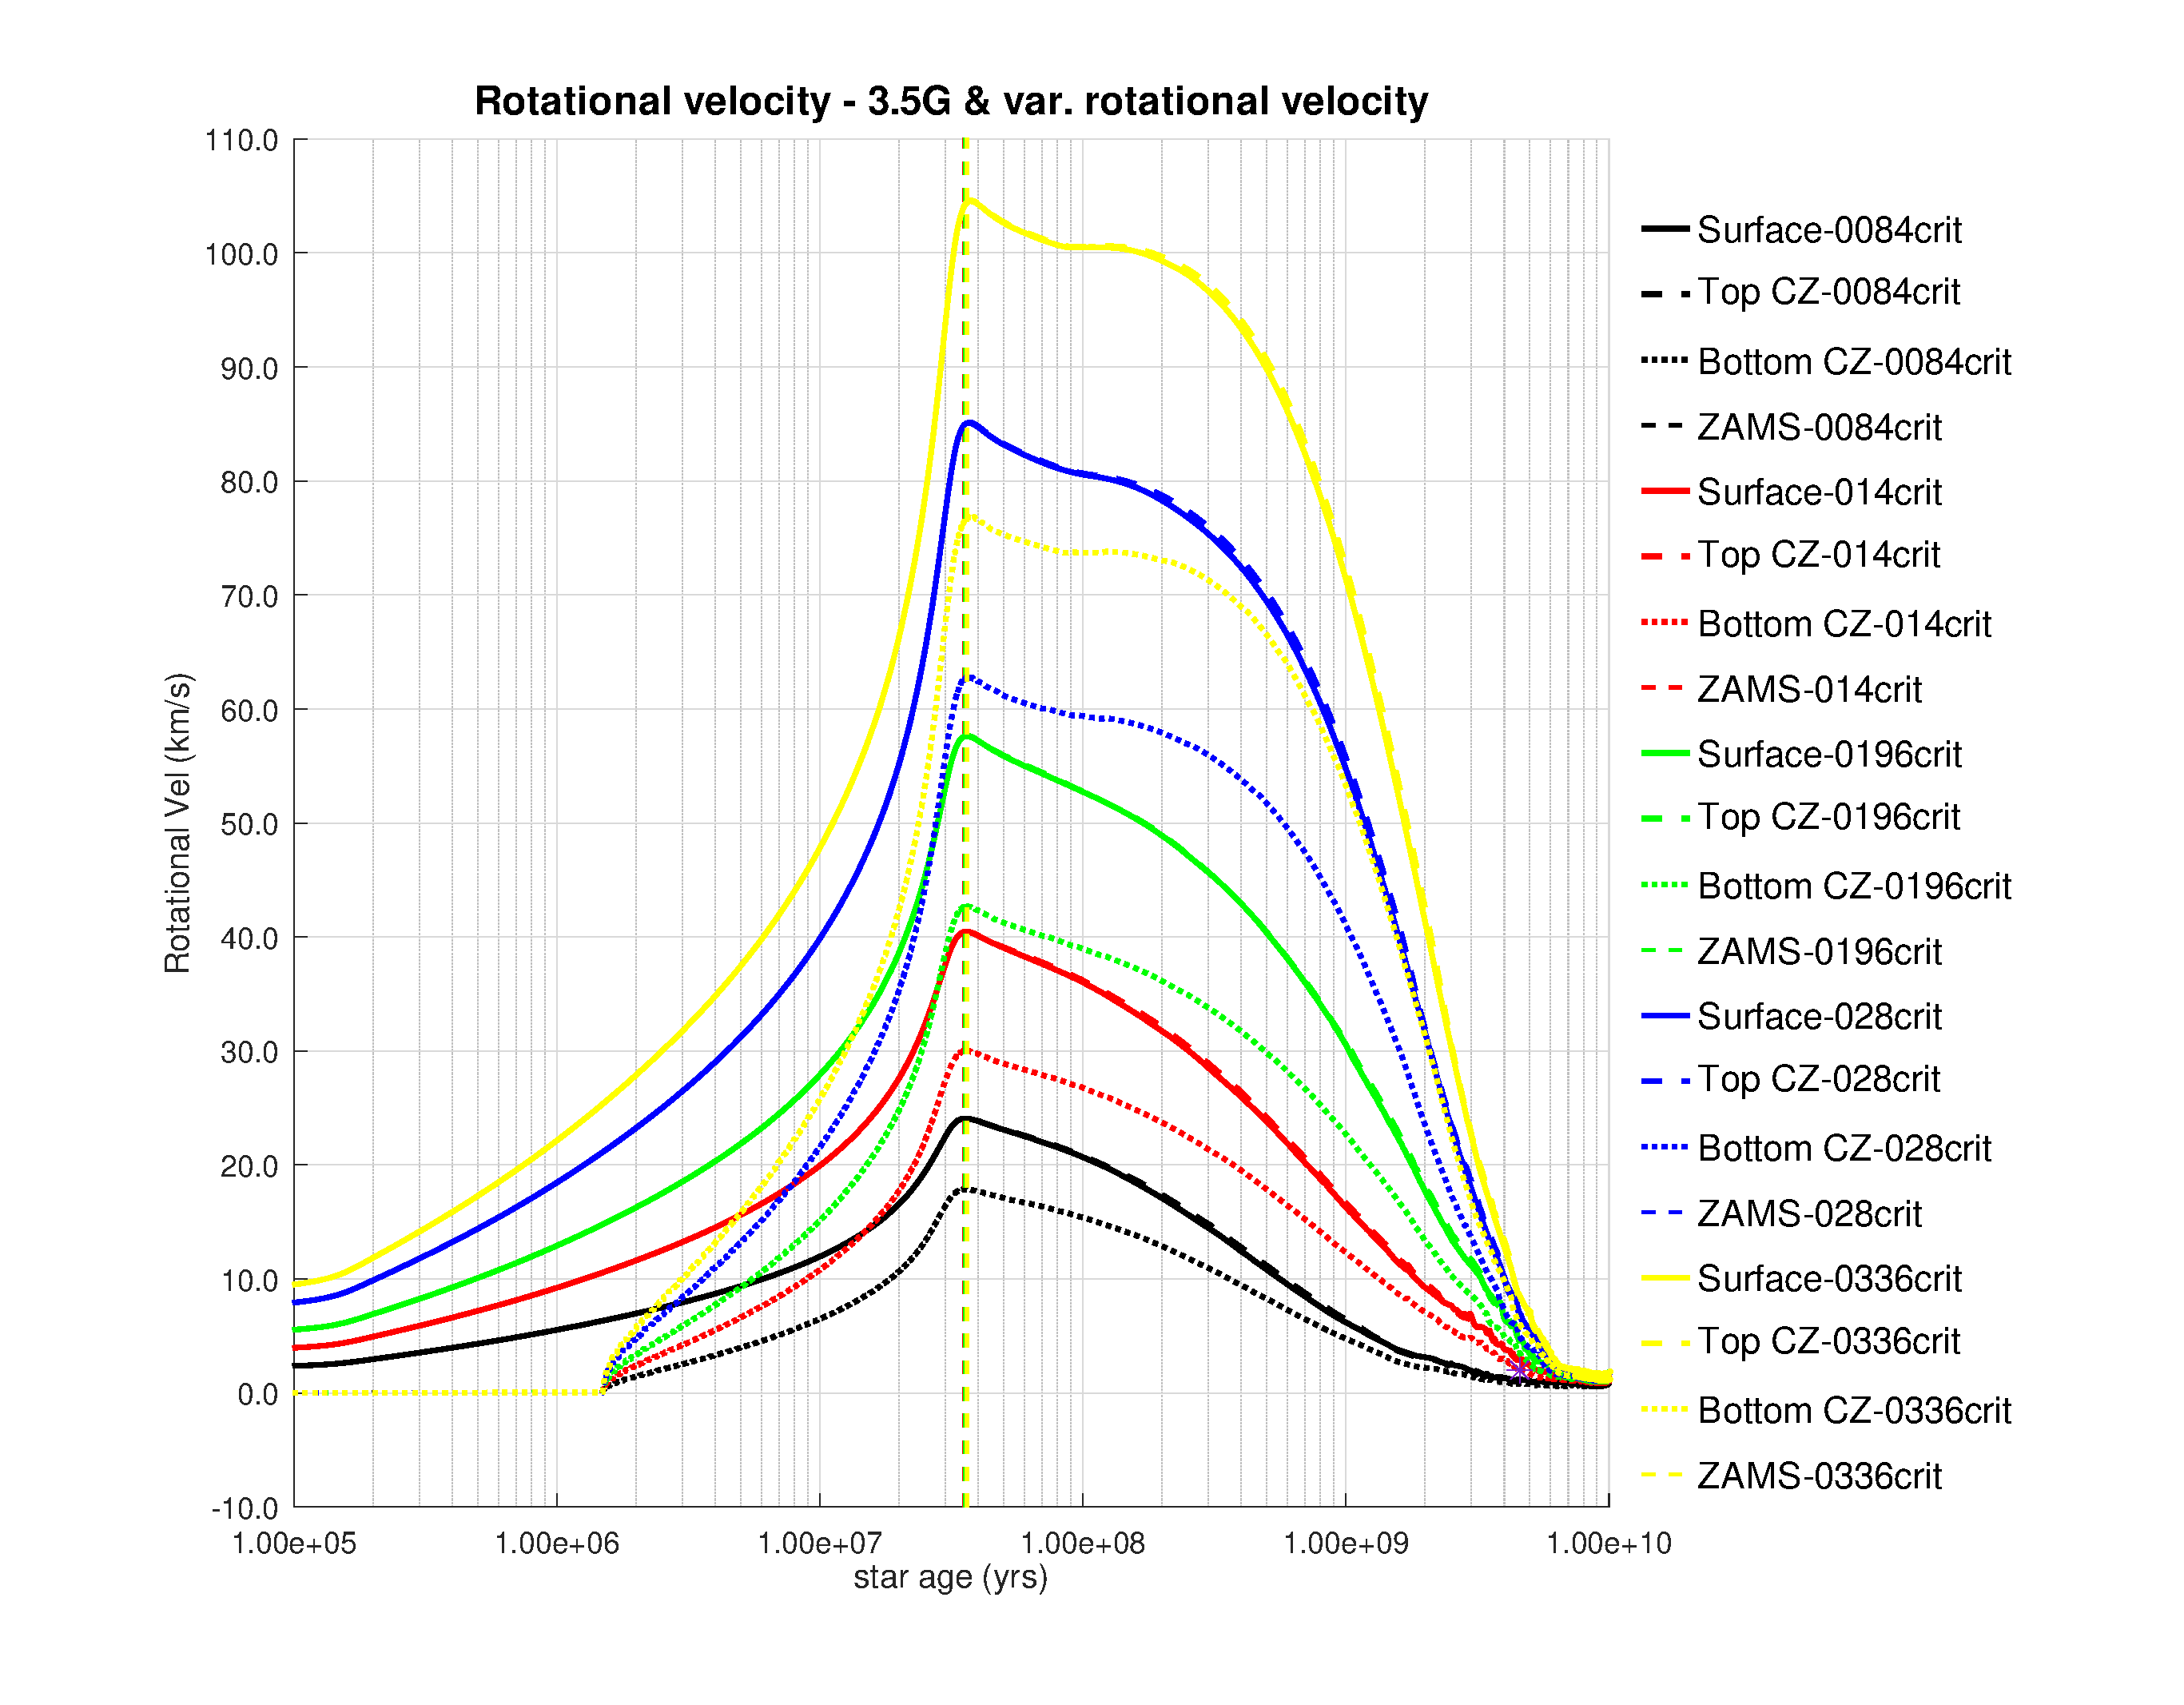
\includegraphics[trim = 30mm 15mm 20mm 15mm, clip,width=\textwidth]{figures/rot_vel_var_vel_3_5g.eps}
    \label{fig:subim43}
    \end{subfigure}
    \begin{subfigure}[h]{0.47\textwidth}
    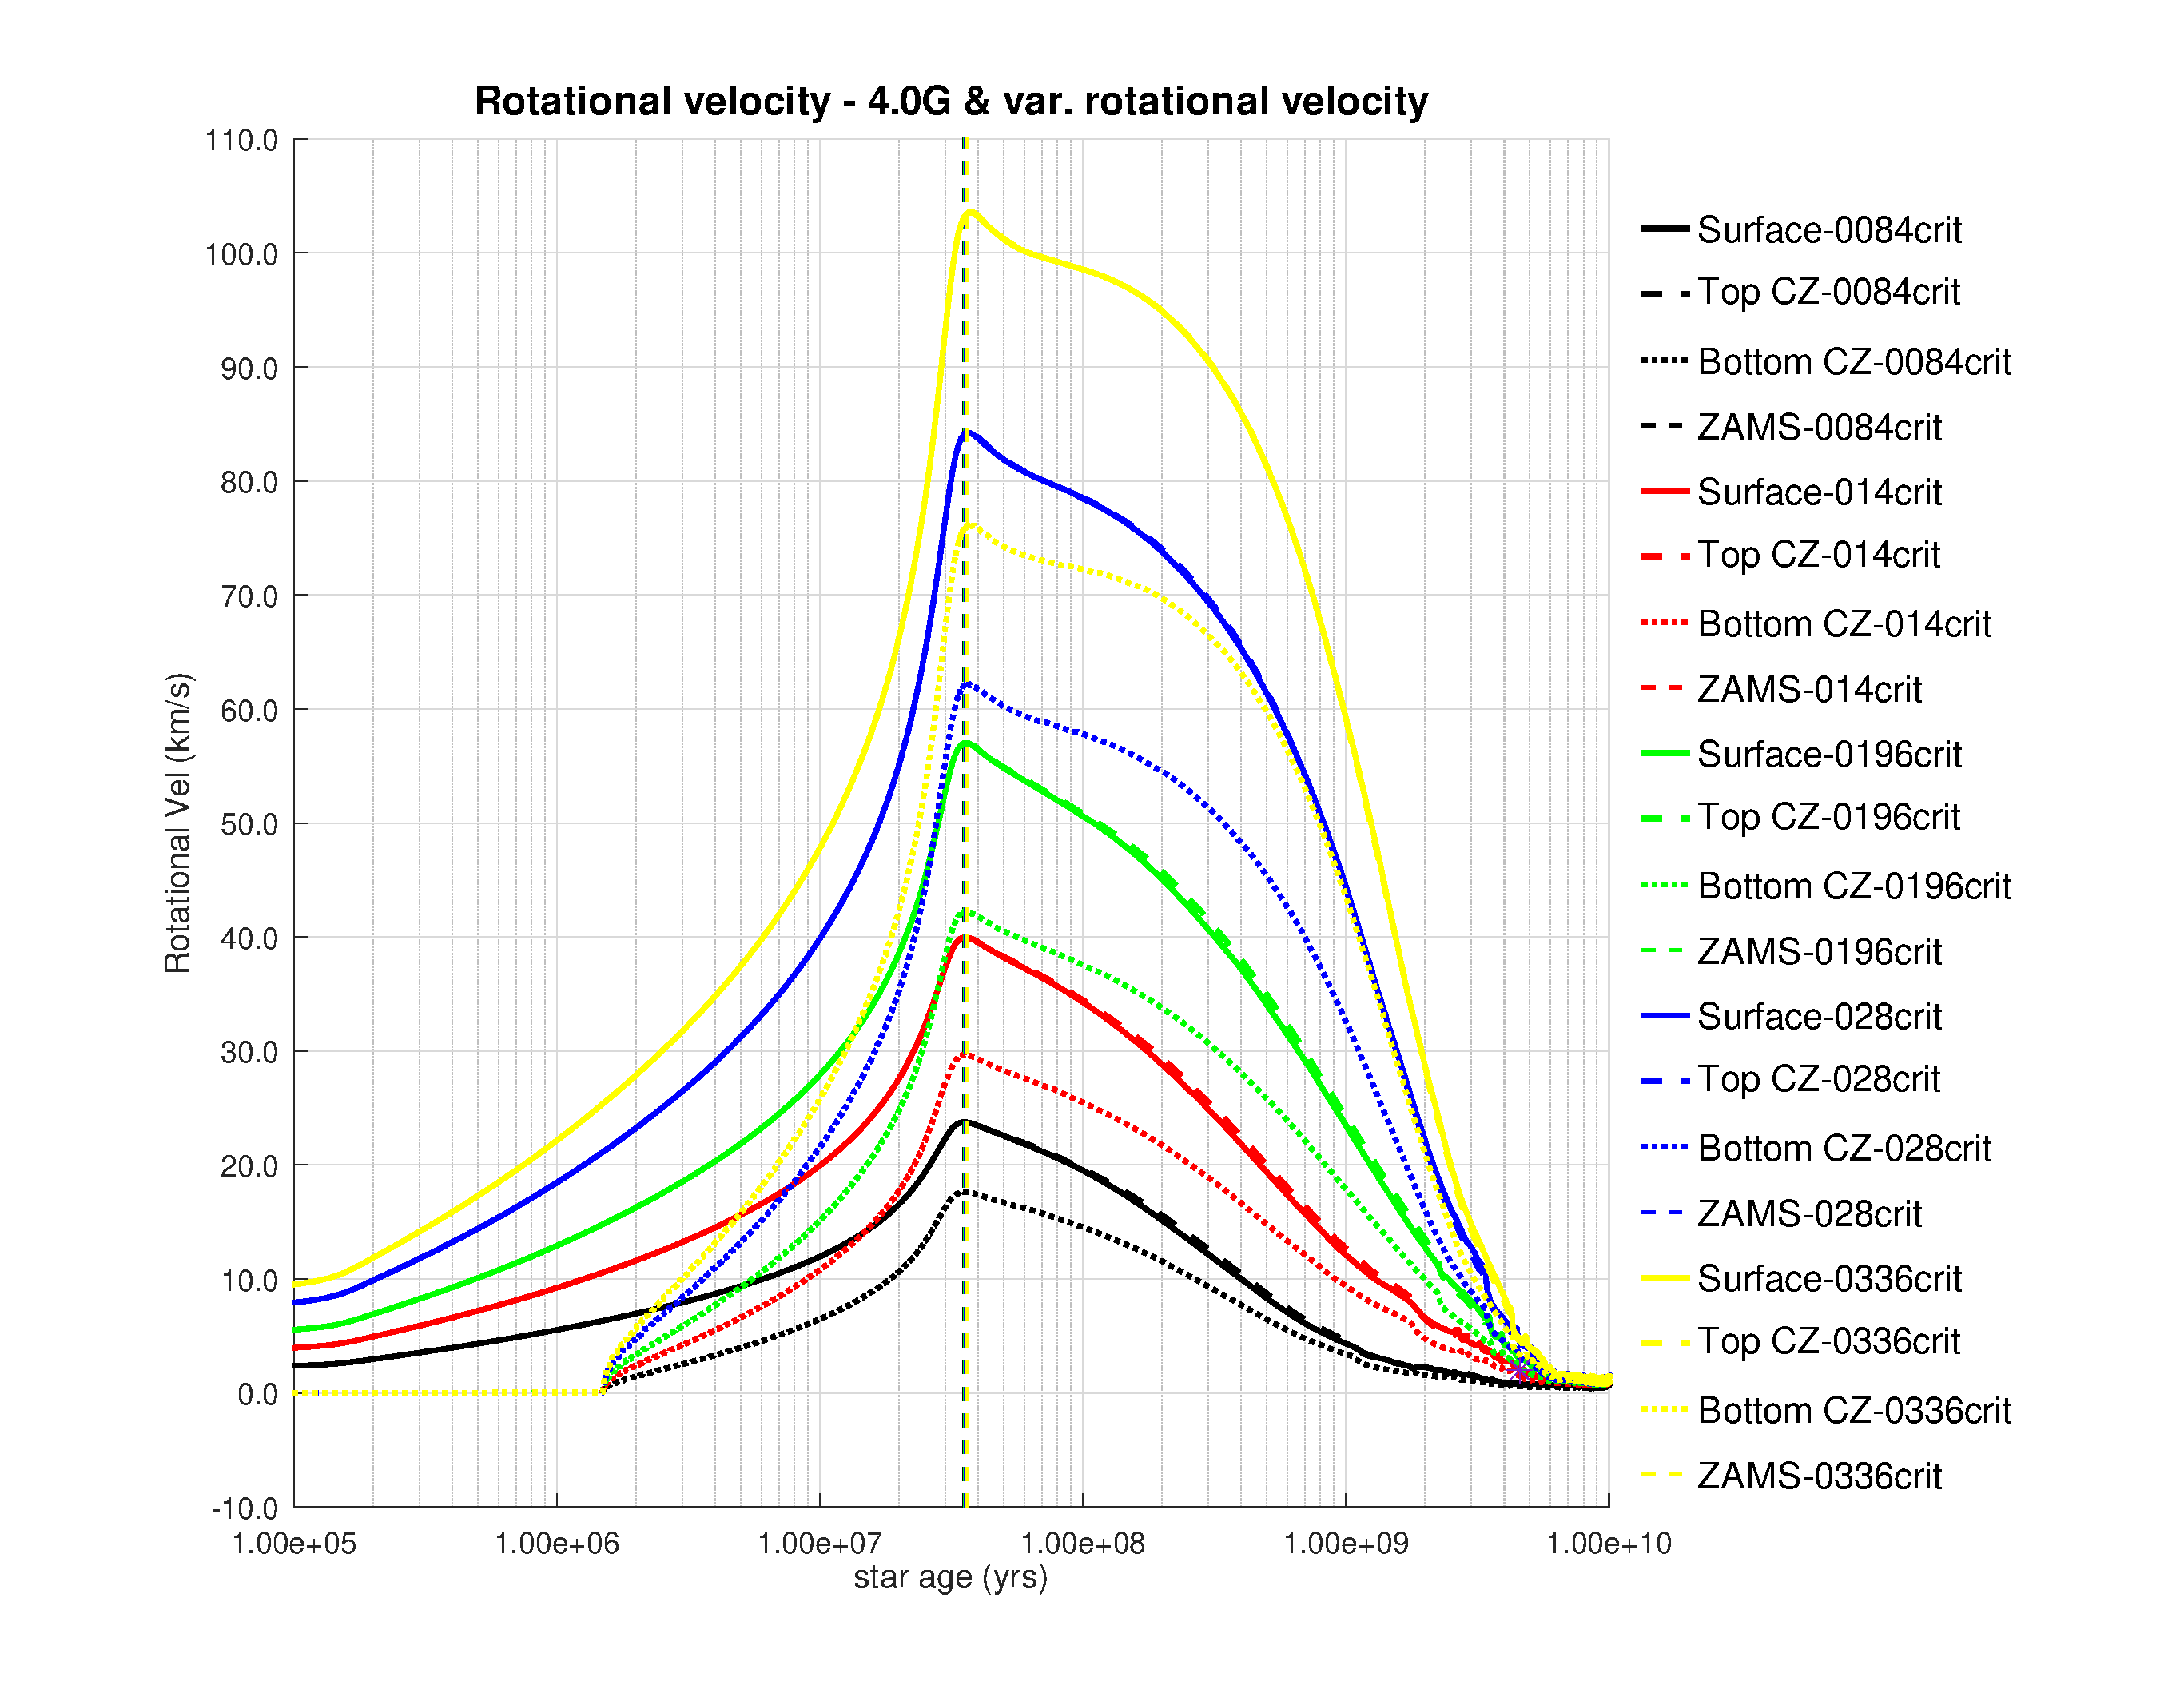
\includegraphics[trim = 30mm 15mm 20mm 15mm, clip,width=\textwidth]{figures/rot_vel_var_vel_4_0g.eps}
    \label{fig:subim44}
    \end{subfigure}
    \begin{subfigure}[h]{0.47\textwidth}
    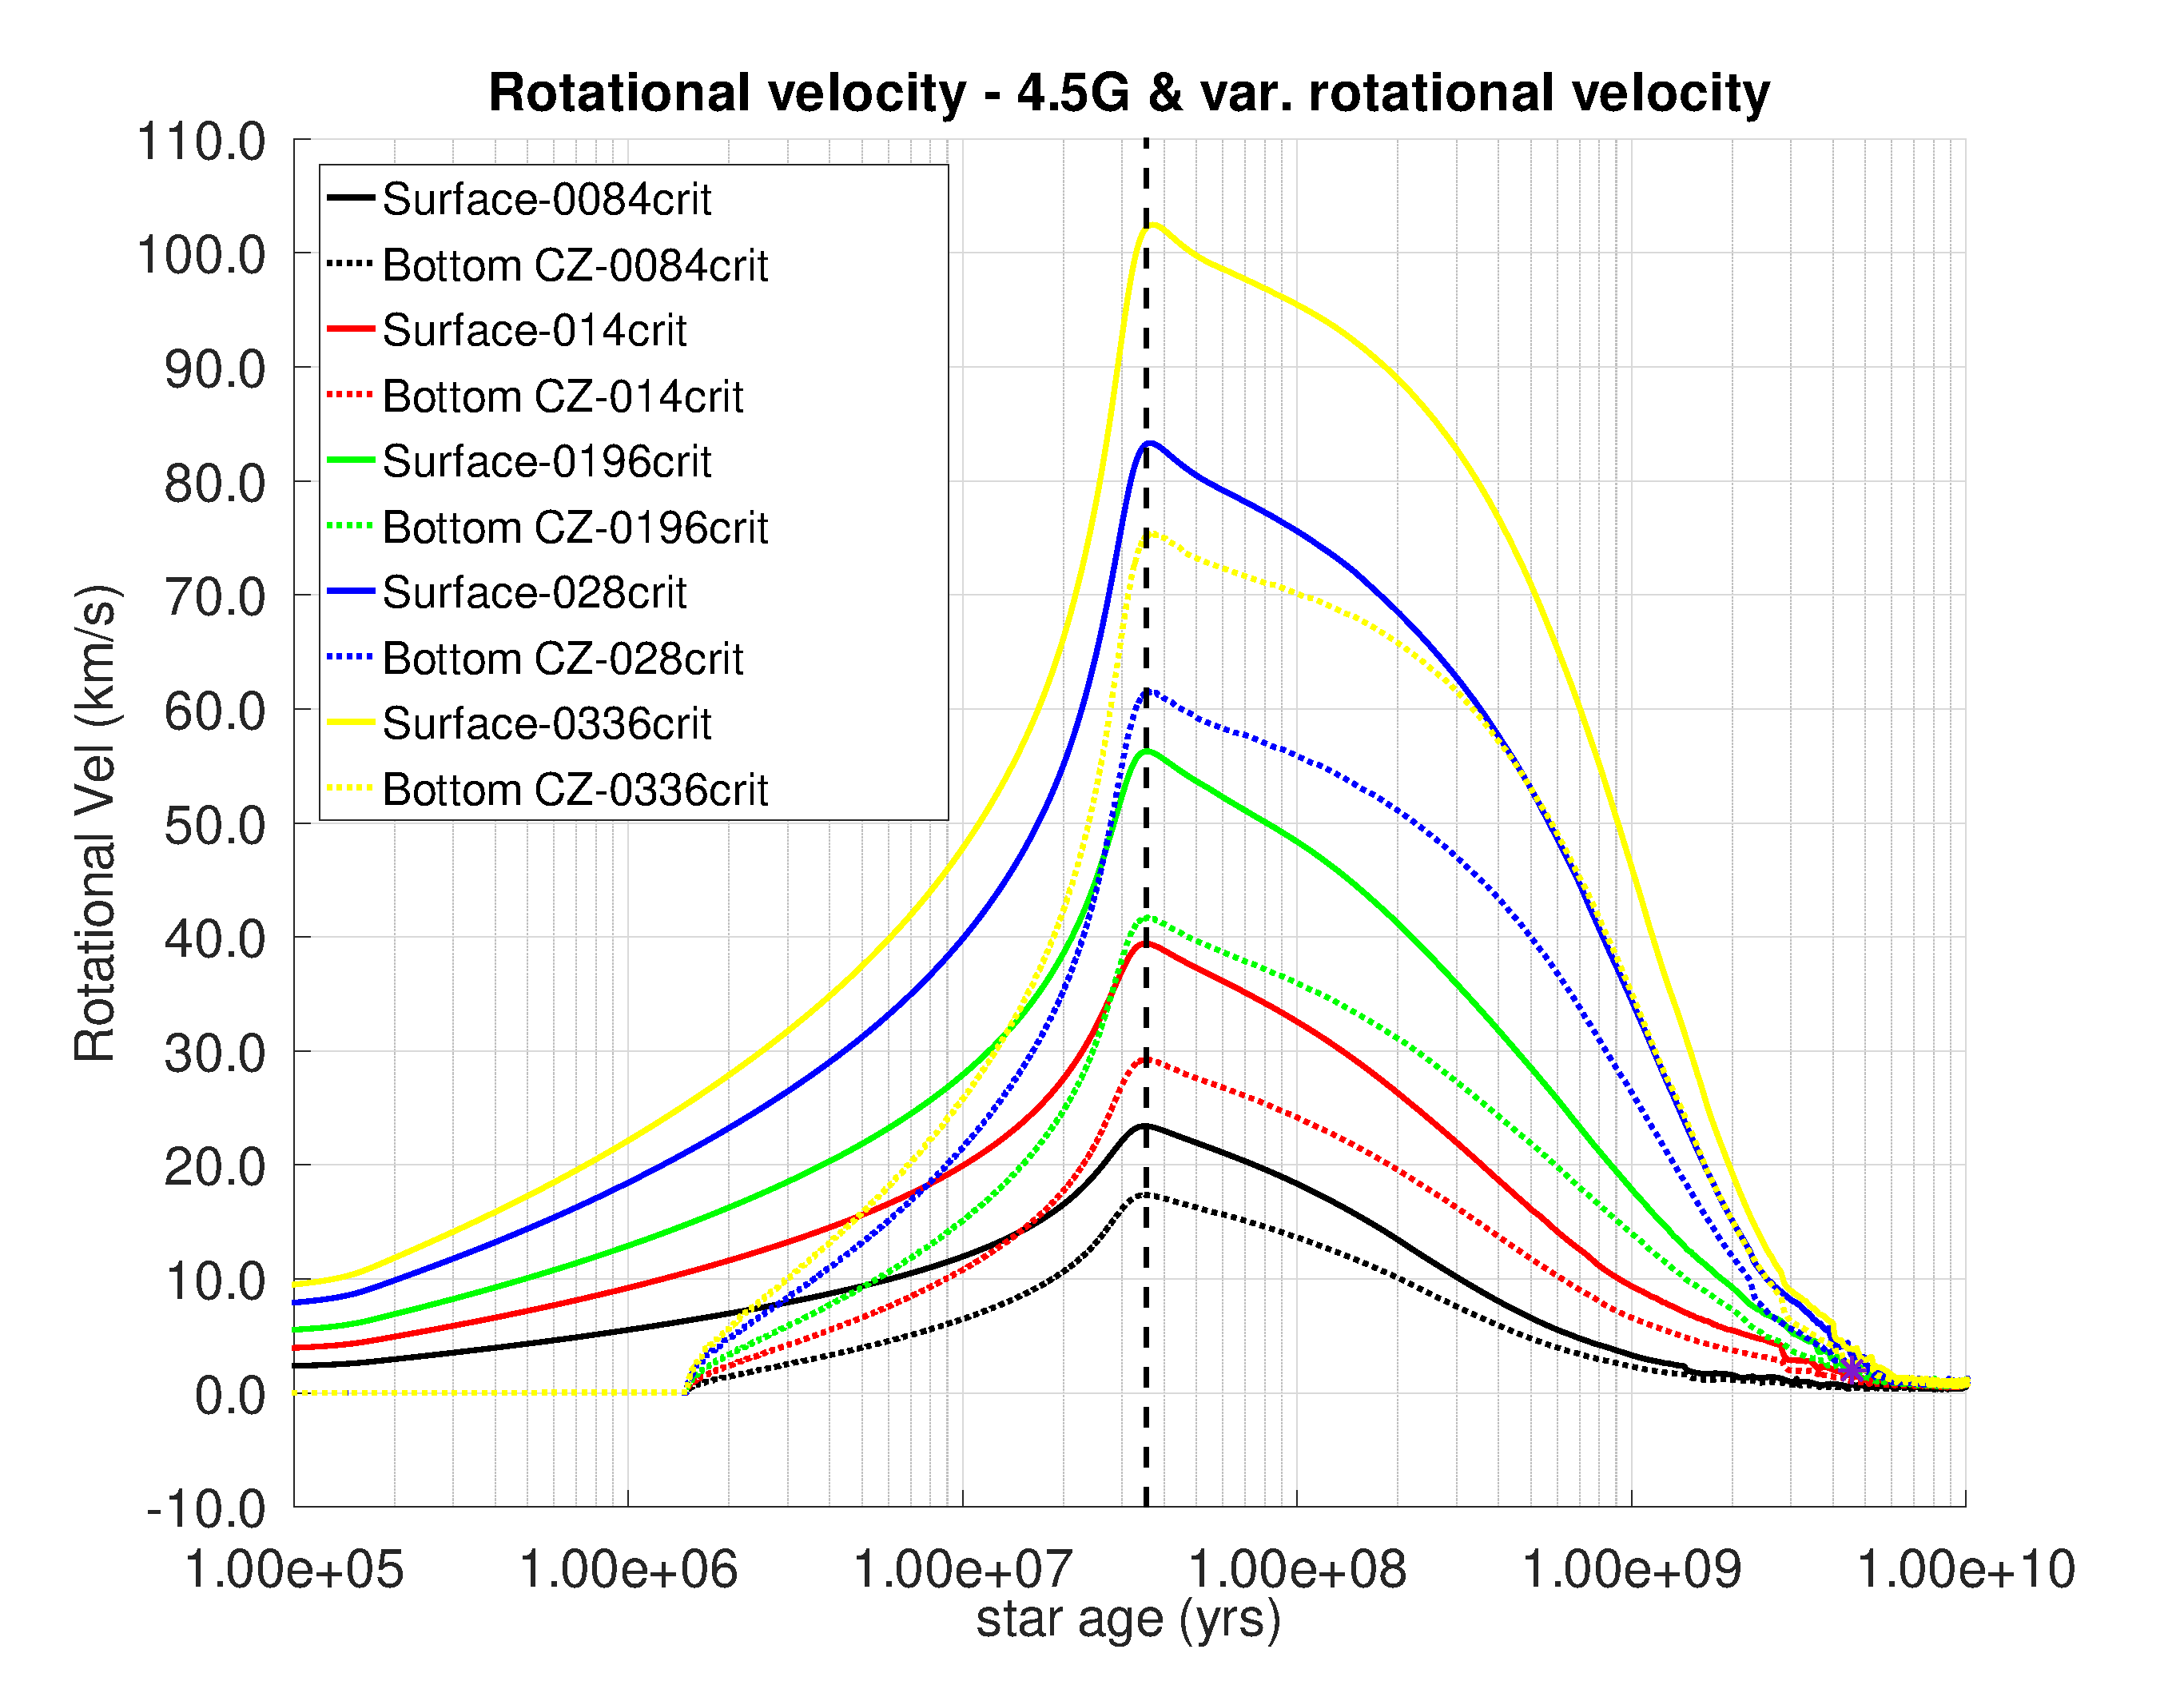
\includegraphics[trim = 30mm 15mm 20mm 15mm, clip,width=\textwidth]{figures/rot_vel_var_vel_4_5g.eps}
    \label{fig:subim45}
    \end{subfigure}
    \begin{subfigure}[h]{0.47\textwidth}
    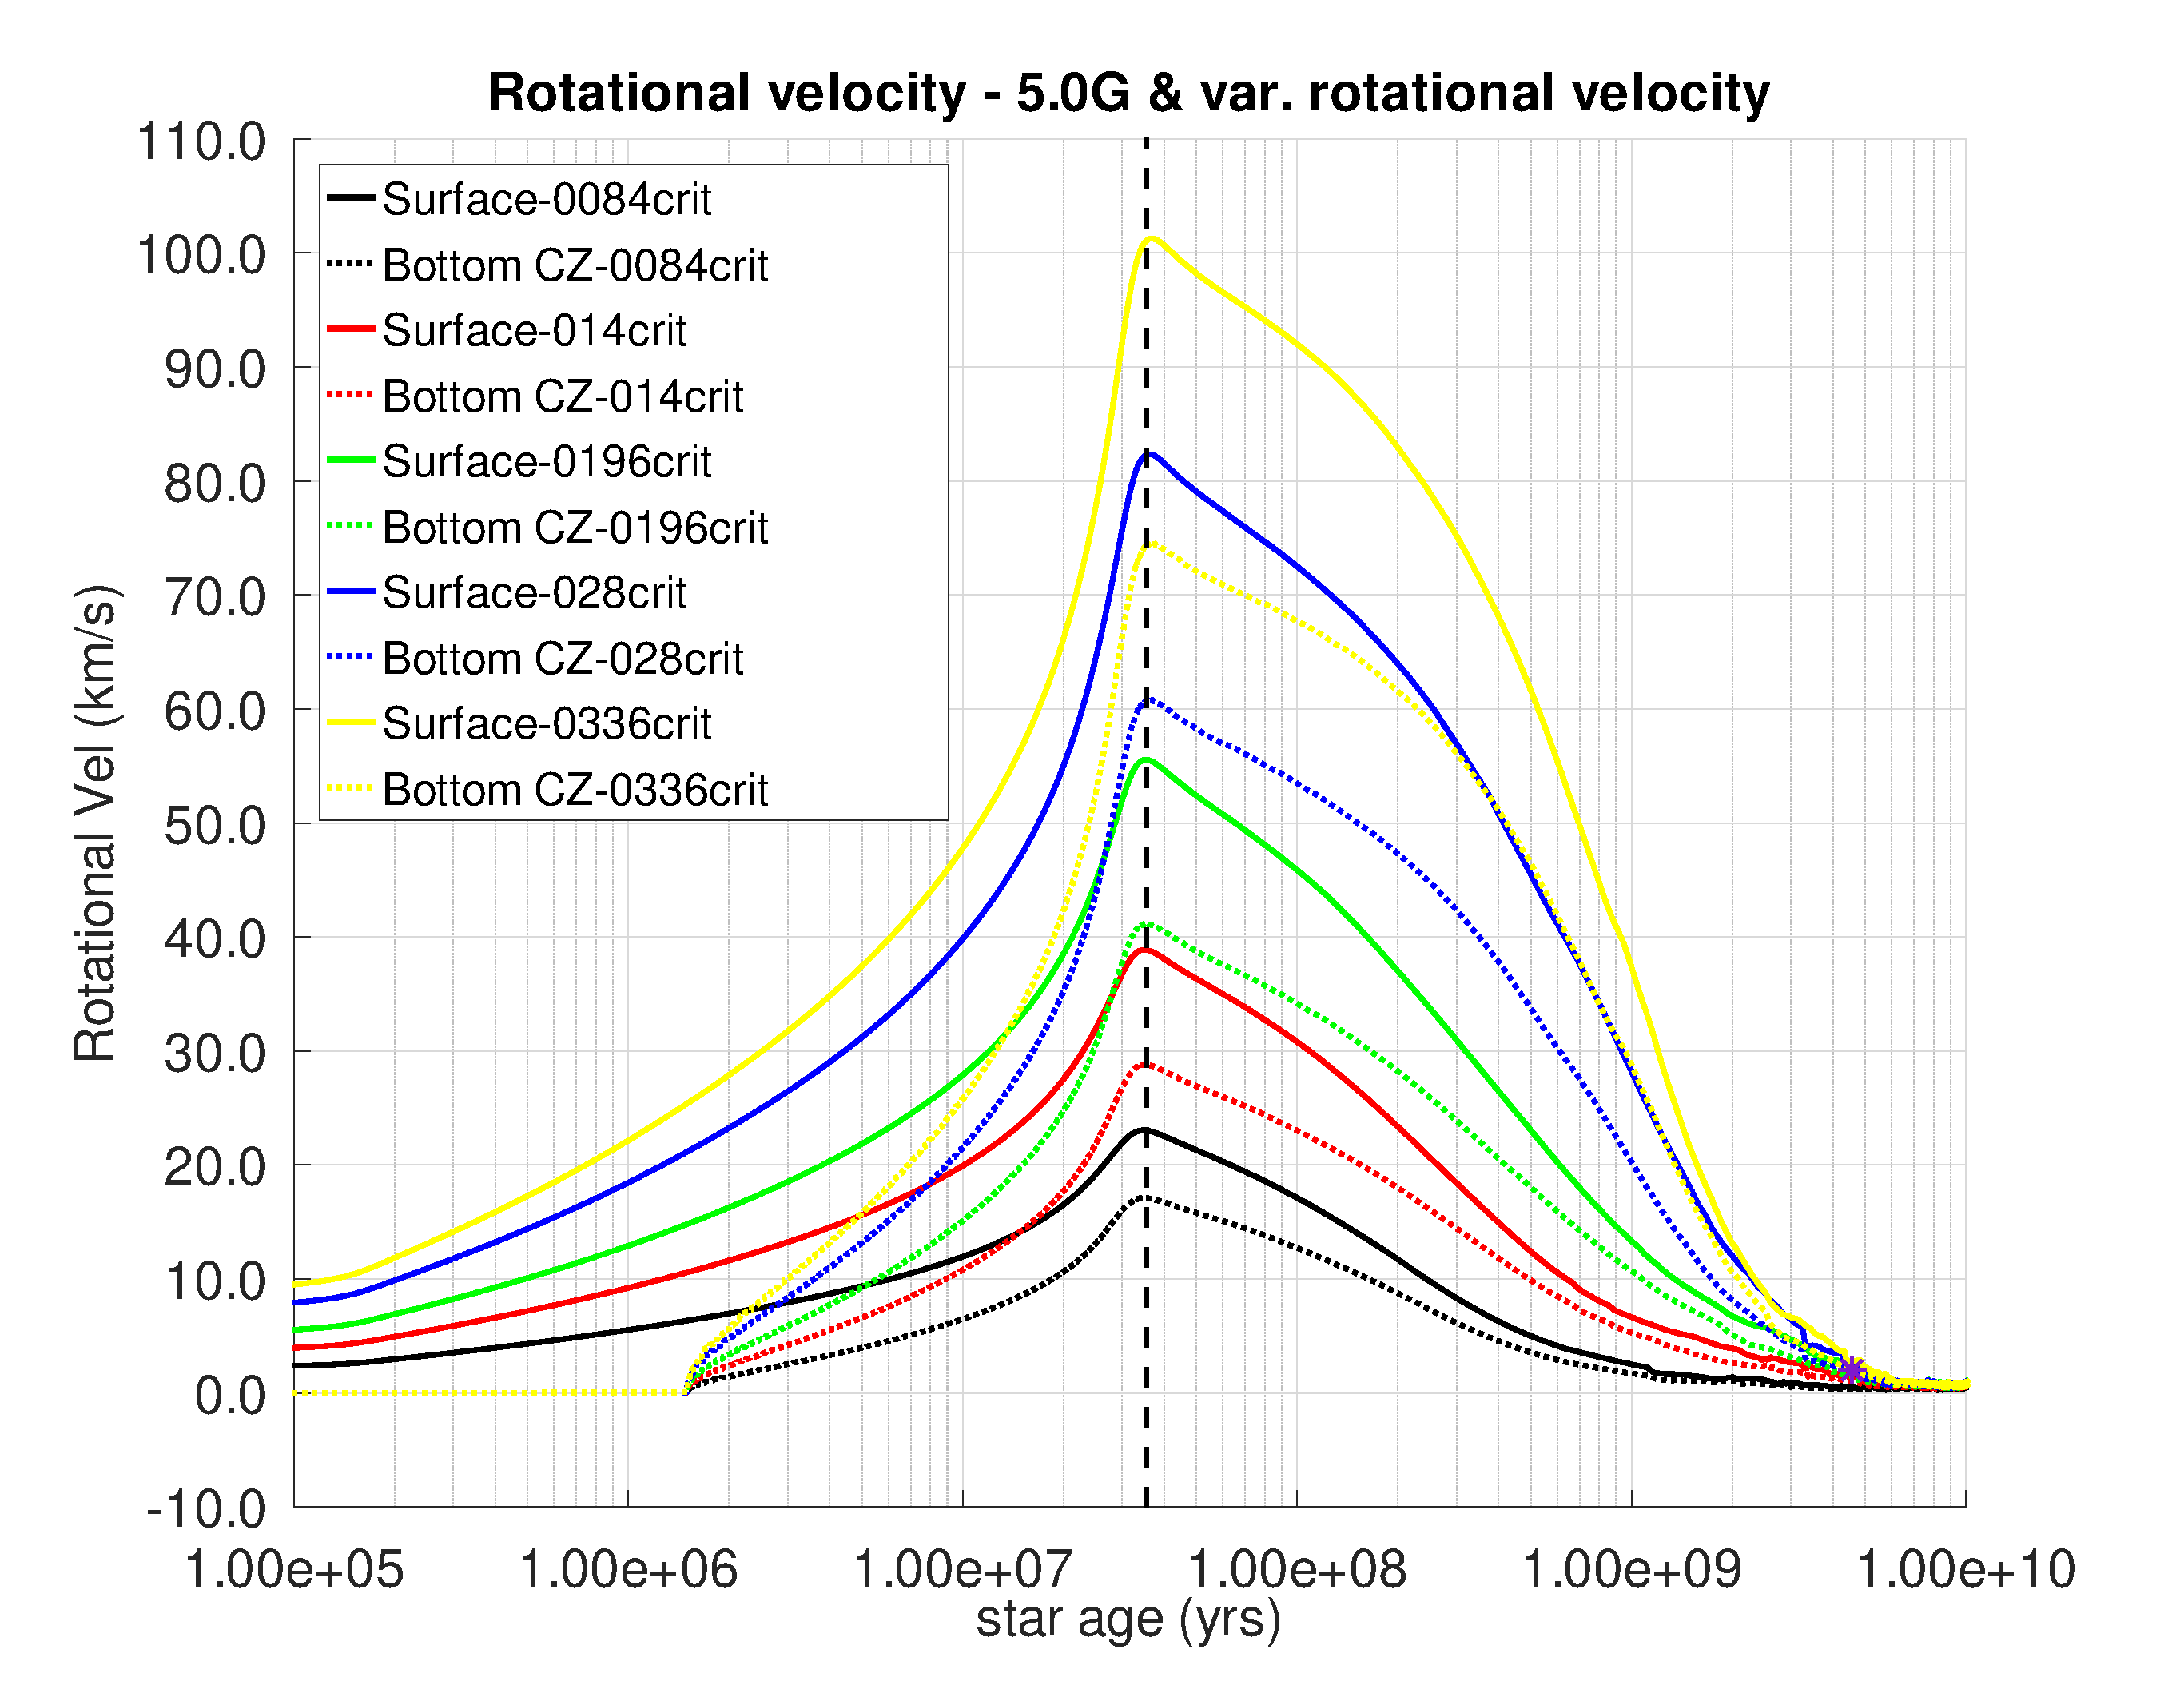
\includegraphics[trim = 30mm 15mm 20mm 15mm, clip,width=\textwidth]{figures/rot_vel_var_vel_5_0g.eps}
    \label{fig:subim46}
    \end{subfigure}
\caption{Grid showing of the evolution of surface rotational velocity, as a function of time for several 1 $\msun$ models. Each figure shows a set of models in which the magnetic field with intensity has been fixed and $\oomegac$ varies between 0.0084 and 0.0336. The purple star is the surface angular velocity for the present-day Sun \citep{Gill2012}. The dashed lines make reference to the ZAMS.}
\label{fig:grid_rot_vel}
\end{figure*}

%%%%%%%%%%%%%%%%%%%%%%%%%%%%%%%%%%%%%%%%%%%%%%%%%%



% Don't change these lines
\bsp	% typesetting comment
\label{lastpage}
\end{document}

% End of mnras_template.tex